\documentclass[11pt]{article}

\usepackage{maiacustom}

\begin{document}

\psettitle{Banco de questões de astronomia}

Estas questões foram produzidas/selecionadas cuidadosamente com o objetivo de preparar os estudantes para o processo seletivo de astronomia no Brasil. Algumas questões não são de autoria própria e estão devidamente sinalizadas por () antes do enunciado. O template do banco de questões é o mesmo do Professor \text{Kevin Zhou}. Seu trabalho é valioso, e diversas ideias desta lista podem ser encontradas em seus Handouts.

% \begin{psidea}{Título da Ideia}{}
% Ideia
% \end{psidea}

% \begin{psexample}{Título do Exemplo}{}
% Exemplo
% \end{psexample}

% \begin{pssolution*}{}{}
% Solução
% \end{pssolution*}

% \begin{psremark*}{Título da Observação}{}
% Observação
% \end{psremark*} 

\section{Mecânica Celeste}
\pts{5}    
\begin{pproblem}
    Iaum e Sevla, dois físicos renomados, pretendem lançar uma sonda espacial para explorar os limites da física newtoniana e as correções relativísticas necessárias nas proximidades de um buraco negro. Eles precisam da sua ajuda para estudar o \textit{Potencial Efetivo} de tal corpo.
    \begin{enumerate}[label=\textbf{\alph*)}]
        \item A energia de um corpo de massa \(m\) orbitando um corpo massivo de massa \(M\) pode ser escrita como:
             \[
             \frac{m\dot r ^2}{2} + V_{eff}(r)
             \]
             Onde \(\dot r\) é a velocidade radial do corpo. Encontre \(V_{eff}(r)\) em função de \(G\), \(M\), \(L\), \(m\) e \(r\).

        \item Segundo a física newtoniana, qual é o menor raio no qual é possível um corpo possuir uma órbita circular em torno de um buraco negro?
    
        \item Qual é a frequência de pequenas oscilações radiais, \(\omega_r\), em torno desse raio?

        O potencial gravitacional próximo a esses corpos precisa sofrer uma correção relativística e tem a forma:
        \[
        V(r) = -\frac{GMm}{r} - \frac{GML^2}{mc^2r^3}
        \]

        \item Explique por que essa correção permite que uma partícula caia no centro de um buraco negro, \(r=0\), e por que isso é impossível na física newtoniana.
        
        \item Qual é o menor valor de \(L\) para que uma partícula possa orbitar o buraco negro em uma órbita circular? Qual é o valor do raio nessa condição?
        
        \item Assumindo \( \lim_{L \to \infty}\), encontre a menor distância que uma partícula em órbita aberta pode se aproximar de um buraco negro.  
    \end{enumerate}
    \begin{pssolution*}{}{}
        \begin{alternativas}
            \item Da forma clássica, temos:
            \[E = \frac{mv^2}{2}-\frac{GMm}{r}\]
            Note que podemos escrever \(v^2 = v_\theta^2+ v_r^2\), onde \(v_\theta\) e \(v_r\) são, respectivamente, as velocidades tangenciais e radiais do corpo. Como \(v_r = \dot{r}\), precisamos encontrar uma expressão que relacione \(v_\theta\) com outra grandeza. A melhor maneira de fazer essa relação é utilizando o momento angular, pois:
            \[L = mrv_\theta \rightarrow v_\theta = \frac{L}{mr}\]
            Substituindo na expressão da energia, temos:
            \[E = \frac{m\dot{r}^2}{2}+\frac{L^2}{2mr^2} - \frac{GMm}{r}\]
            Como queremos uma resposta na forma \(E = m\dot{r}^2/2 + V_{eff}(r)\), por analogia, temos:
            \[\boxed{V_{eff}(r) = -\frac{GMm}{r}+\frac{L^2}{2mr^2}}\]

            \item A maior velocidade limite de um corpo é \(c\), desconsiderando efeitos relativísticos:
            \[\frac{mc^2}{2}-\frac{GMm}{R} = -\frac{GMm}{2R}\]
            Isolando \(R\):
            \[\boxed{R = \frac{GM}{c^2}}\]

            \item Para pequenas oscilações, temos a aproximação:
            \[\omega_r \approx \sqrt{\frac{V_{eff}''(R)}{m}}\]
            Calculando:
            \[V_{eff}'(R) = \frac{GMm}{r^2}-\frac{L^2}{mr^3}\]
            \[V_{eff}''(R) = -\frac{2GMm}{r^3}+\frac{3L^2}{mr^4}\]
            Utilizando que \(L = mvr\) (órbitas circulares) e que \(v\equiv c\), chegamos a:
            \[V_{eff}''(R) = \frac{mc^6}{G^2M^2}\]
            Com isso, podemos concluir que:
            \[\omega_r = \frac{c^3}{GM}\]

            \item Quando tomamos o limite de \(\lim_{r\rightarrow 0}V_{eff}(r)\), na física newtoniana, o termo que domina é \(L^2/2mr^2\), ou seja, seria necessária uma energia \(+\infty\) para chegar ao centro do buraco negro. No entanto, após a correção relativística, o termo que domina é \(-GML^2/mc^2r^3\), ou seja, seria necessária uma energia de \(-\infty\) para chegar ao centro do buraco negro. Por isso, não é possível chegar ao centro de um buraco negro na física newtoniana.
            
            \item Em uma órbita circular, \(r\) é constante, o que implica que a força na direção radial é nula, ou seja:
            \[V_{eff}'(r) = 0\]
            Calculando:
            \[V_{eff}'(r) = \frac{GMm}{r^2}-\frac{L^2}{mr^3}+\frac{3GML^2}{mc^2r^4}=0\]
            Simplificando, temos:
            \[r^2-\frac{L^2}{GMm^2}r+\frac{3L^2}{m^2c^2}=0\]
            Note que a solução dessa equação precisa ser real, uma vez que \(r\) não pode ser imaginário, o que nos impõe a condição:
            \[\frac{L^4}{G^2M^2m^4} - \frac{12L^2}{m^2c^2} \geq 0\]
            Na condição de igualdade, o valor de \(L\) que satisfaz essa equação é:
            \[\boxed{L = \frac{\sqrt{12}GMm}{c}}\]
            O valor de \(r\) nesse caso é:
            \[r = \frac{L^2}{2GMm^2} = \boxed{r_{min} = \frac{6GM}{c^2}}\] 
            
            \item A expressão completa para \(r\) é:
            \[r = \frac{\frac{L^2}{GMm^2}\pm\sqrt{\left(\frac{L^2}{GMm^2}\right)^2-\frac{12L^2}{m^2c^2}}}{2} = \frac{L^2-\sqrt{L^4-12(GMmL/c)^2}}{2GMm^2}\] 
            No limite de \(L\rightarrow \infty\), temos:
            \[r_{min} = \lim_{L \rightarrow \infty}\frac{L^2-\sqrt{L^4-12(GMmL/c)^2}}{2GMm^2} = \frac{6(GMm/c)^2}{2(GMm^2)} = \boxed{\frac{3GM}{c^2}} \] 
        \end{alternativas}
    \end{pssolution*}
\end{pproblem}

\pts{3}
\begin{pproblem} Um ponto importante no estudo de órbitas é o que acontece quando o potencial segue algo incomum. O objetivo desta questão é estudar esse fenômeno. Considere o momento angular \(L\) e a massa do corpo \(m\).
    \begin{alternativas}
        \item Para uma órbita geral, que possui um potencial \(V(r)\) na forma \(\psi r^k\), encontre o valor \(r_0\) de uma órbita circular para esse potencial.
        
        \item Encontre a frequência de pequenas oscilações, \(\omega_r\), em torno desse raio. 
        
        \item Seja \(\omega_\theta\) a frequência angular da órbita, encontre o valor da razão \(\frac{\omega_r}{\omega_\theta}\). Uma órbita só pode ser fechada se essa razão for um número inteiro. Por quê? Encontre valores de \(k\) para que a órbita seja fechada.
         
    \end{alternativas} 

    \begin{pssolution*}{}{}
        \begin{alternativas}
            \item Como em uma órbita circular \(V_{eff}'(r) = 0\), temos:
            \[V_{eff}'(r) = -\frac{L^2}{mr^3}+k\psi r^{k-1} = 0\]
            \[k\psi r^{k-1} = \frac{L^2}{mr^3} \rightarrow \boxed{r_0 = \left(\frac{L^2}{k\psi m}\right)^{\frac{1}{k+2}}}\]
        
            \item Utilizando que \(\omega_r^2=V_{eff}''(r_0)/m\):
            \[V_{eff}''(r) = \frac{3L^2}{mr^4}+k(k-1)\psi r^{k-2}\]
            \[V_{eff}''(r) = r^{-4}\left(\frac{3L^2}{m}+k(k-1)\psi r^{k+2}\right)\]
            \[V_{eff}''(r) = r^{-4}\left(\frac{3L^2}{m}+k(k-1)\psi \frac{L^2}{k\psi m}\right)\]
            \[V_{eff}''(r) = \frac{L^2}{r_0^4m}(k+2)\]
            Assim, temos:
            \[\boxed{\omega_r = \frac{L^2}{r_0^2m}\sqrt{k+2}}\]

            \item Pela definição de \(L\), temos:
            \[L = mr_0^2\omega_\theta \rightarrow \omega_\theta = \frac{L^2}{mr_0^2}\]
            Portanto:
            \[\frac{\omega_r}{\omega_\theta} = \sqrt{k+2}\]
            Note que, para a órbita ser uma figura fechada, essa razão deve ser um número inteiro, logo, \(k+2\) deve ser um quadrado perfeito. Qualquer valor \(k = n^2-2 \ \forall \ n \in \mathbb{N}\) satisfaz essa equação.
        \end{alternativas}
    \end{pssolution*}
\end{pproblem}

\pts{4} %semana 114
\begin{pproblem}
    O Hodógrafo é uma das maneiras menos conhecidas de resolver questões de mecânica celeste. Ao usar esse mecanismo, é possível resolver questões complexas (envolvendo encontrar parâmetros orbitais, parâmetros de velocidade e como minimizar a excentricidade de uma órbita, por exemplo). Apesar de o Hodógrafo possuir diversas utilidades, o objetivo deste exercício é provar o Teorema do Hodógrafo, que diz que, em órbitas fechadas, a velocidade forma um círculo no espaço vetorial. Vamos provar esse teorema de duas maneiras.
    \begin{align*}
    \textbf{Método 1)}
    \end{align*}
    \begin{enumerate}[label=\textbf{\Roman*.}]
        \item Partindo da Segunda Lei de Newton e da conservação do momento angular, encontre uma expressão para \(d\mathbf{v}/d\theta\). Deixe sua resposta em função do momento angular por unidade de massa, \(h\), e \(\mu\) = \(GM\). 
        \item Onde o centro desse círculo está localizado? Considerando o corpo central na origem do sistema, determine uma expressão para a distância entre o corpo central e o centro do Hodógrafo. 
    \end{enumerate}
    
    \begin{align*}
        \textbf{Método 2)}
    \end{align*}
    O método 2 utiliza noções de cálculo mais avançadas e parte da conservação do \textit{vetor de Laplace-Runge-Lenz}, \(\mathbf{A}\).
    \begin{enumerate}[label=\textbf{\Roman*.}]
        \item O vetor \(\mathbf{A}\) é dado pela expressão:
        \[
        \mathbf{A} = \mathbf{p}\times \mathbf{L} - GMm^2\mathbf{\hat{r}}
        \]
        O primeiro passo para a demonstração é provar que \(\mathbf{A}\) é constante. Para isso, derive o mesmo em relação ao tempo e tire suas próprias conclusões.
        \item Como o vetor \(\mathbf{L}\) é constante, \(\mathbf{A}\times\mathbf{L}\) também é uma constante. Utilizando a identidade vetorial \(\mathbf{A}\times(\mathbf{B}\times\mathbf{C}) = \mathbf{B}(\mathbf{A}\cdot\mathbf{C}) - \mathbf{C}(\mathbf{A}\cdot\mathbf{B}) \), prove que \(\mathbf{v}\) forma um círculo no espaço vetorial.    
    \end{enumerate}
    \begin{pssolution*}{}{}
        \textbf{Método 1)}

        \begin{enumerate}[label=\textbf{\Roman*.}]
            \item A Segunda Lei de Newton nos diz que:
            \[-\frac{GMm}{r^2}\mathbf{\hat{r}} =  m\frac{d\mathbf{v}}{dt}\]
            Pela definição de momento angular:
            \[L = mr^2\frac{d\theta}{dt} \rightarrow \ \  \therefore dt = \frac{mr^2}{L}d\theta\]
            Substituindo \(dt\) na fórmula da Segunda Lei de Newton:
            \[-\frac{GMm}{r^2}\mathbf{\hat{r}} = m\left(\frac{L}{mr^2}\right)\frac{d\mathbf{v}}{d\theta}\]

            Isolando \(dv/d\theta\), temos:

            \[\boxed{\frac{d\mathbf{v}}{d\theta} = -\frac{GMm}{L}\mathbf{\hat{r}} \equiv -\frac{\mu}{h}\mathbf{\hat{r}}}\]

            Note que essa expressão é um círculo no espaço vetorial e possui raio \(R = \mu/h\), uma vez que \(d\mathbf{v}/d\theta\) é constante e aponta na direção radial.

            \item Como vimos no item anterior, o hodógrafo forma um círculo de raio \(R = \mu/h\). Tome como apoio a seguinte imagem:
            \begin{figure}[H]
                \centering
                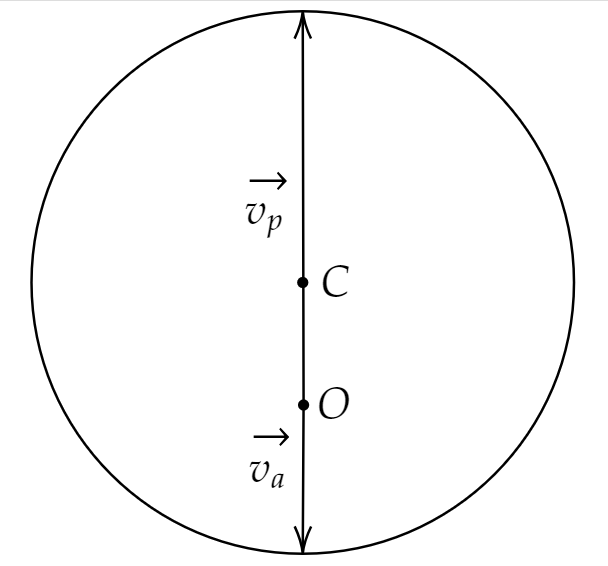
\includegraphics[width=0.4\linewidth]{imagens/hodografo1.png}
                \caption{Esquema do Hodógrafo}
            \end{figure}
            O ponto \(O\) representa a origem do sistema (local do corpo central). Note que a menor distância entre \(O\) e o Hodógrafo deve corresponder à menor velocidade (apoastro) e a maior distância deve corresponder à maior velocidade (periastro). Note também que \(v_a + \overline{OC} = v_p - \overline{OC}\). Equacionando, temos:
            \[v_a + v_p = 2R \equiv \frac{2\mu}{h}\]
            \[v_p - v_a = 2\overline{OC}\]

            Podemos escrever \(v_p\) e \(v_a\) em função do momento angular:
            \[L = ma(1-e)v_p \rightarrow v_p = \frac{h}{a(1-e)}\]
            \[L = ma(1+e)v_a \rightarrow v_a = \frac{h}{a(1+e)}\]
            
            Substituindo na primeira equação:
            \[\frac{h}{a}\left(\frac{1}{1+e}+\frac{1}{1-e}\right) = \frac{2\mu}{h}\]
            
            Aqui, podemos isolar \(a\):
            \[\frac{h}{a}\left(\frac{2}{(1-e)^2}\right) = \frac{2\mu}{h}\]

            \[a = \frac{h^2}{\mu}\frac{1}{(1-e)^2}\]

            Com isso em mente, podemos ir para a segunda expressão:
            \[\frac{h}{a}\left(\frac{1}{1-e}-\frac{1}{1+e}\right) = 2\overline{OC}\]
            \[h\left(\frac{\mu(1-e)^2}{h^2}\right)\left(\frac{2e}{(1-e)^2}\right) = 2\overline{OC}\]
            
            Finalmente, resolvendo para \(\overline{OC}\), temos:
            \[\boxed{\overline{OC} = \frac{\mu}{h}e}\]

            Para uma elipse (\(e<1\)), a origem fica dentro da circunferência; para uma parábola (\(e=1\)), a origem fica no limite da circunferência; e para uma hipérbole (\(e>1\)), a origem fica fora da circunferência.
        \end{enumerate}

    
        \textbf{Método 2}
        \begin{enumerate}[label=\textbf{\Roman*.}]
            \item Derivando \(\mathbf{A}\) em relação ao tempo, temos:
            \[\frac{d\mathbf{A}}{dt} = \frac{d}{dt}(\mathbf{p}\times\mathbf{L}) - GMm^2\frac{d}{dt}\mathbf{\hat{r}}\] 
            Quando derivamos um \textit{versor} em relação ao tempo, temos:
            \[\frac{d\mathbf{\hat{r}}}{dt} = \mathbf{\omega}\times\mathbf{\hat{r}}\]
            Onde \(\mathbf{\omega}\) é a velocidade com que o versor translada. Assim:
            \[\frac{d\mathbf{A}}{dt} = \left(\frac{d\mathbf{p}}{dt}\right)\times \mathbf{L} + \mathbf{p}\times\left(\frac{d\mathbf{L}}{dt}\right) - GMm^2(\mathbf{\omega}\times \mathbf{\hat{r}})\]
            Agora, temos algumas considerações. Primeiramente, note que \(d\mathbf{L}/dt=0\), uma vez que só há forças centrais na órbita. Em segundo lugar, \(d\mathbf{p}/dt = \mathbf{F}\). Além disso, temos que \(\mathbf{L} = mr^2\mathbf{\omega}\). Voltando para a equação:

            \[\frac{d\mathbf{A}}{dt} = -\frac{GMm}{r^2}\mathbf{\hat{r}}\times(mr^2\mathbf{\omega}) - GMm^2(\mathbf{\omega} \times \mathbf{\hat{r}})\]
            \[\frac{d\mathbf{A}}{dt} = -GMm^2(\mathbf{\hat{r}}\times\mathbf{\omega})- GMm^2(\mathbf{\omega} \times \mathbf{\hat{r}})\]

            Para quaisquer dois vetores, \(\mathbf{i}\) e \(\mathbf{j}\), vale que:
            \[i\times j = -j\times i\]

            Utilizando tal propriedade, podemos concluir que:

            \[\boxed{\frac{d\mathbf{A}}{dt} = 0}\]

            Logo, \(\mathbf{A}\) é constante!

            \item Escrevendo a expressão e utilizando o \textit{BAC-CAB}, temos:
            
            \[\mathbf{A}\times\mathbf{L} = (\mathbf{p}\times\mathbf{L})\times\mathbf{L} - GMm^2\mathbf{\hat{r}}\times\mathbf{L}\]

            \[(\mathbf{A} +GMm^2\mathbf{\hat{r}})\times\mathbf{L} = - \mathbf{L}\times(\mathbf{p}\times\mathbf{L}) = \mathbf{p}(-\mathbf{L}\cdot\mathbf{L})-\mathbf{L}(-\mathbf{L}\cdot\mathbf{p})\]

            Como \(\mathbf{L}\) e \(\mathbf{p}\) são sempre perpendiculares, \(\mathbf{L}\cdot\mathbf{p}=0\), assim:

            \[(\mathbf{A}+GMm^2\mathbf{\hat{r}})\times\mathbf{L} = -mL^2\mathbf{v}\]

            Como tanto \(\mathbf{A}\) quanto \(\mathbf{\hat{r}}\) são perpendiculares a \(\mathbf{L}\) e constantes, \(\mathbf{A}+GMm^2\mathbf{\hat{r}}\) traçam um círculo. O produto vetorial com \(\mathbf{L}\) apenas gira o círculo em \(90^\circ\) e multiplica seu raio por \(\mathbf{L}\). Portanto, \(\mathbf{v}\) traça um círculo no espaço vetorial.
            
        \end{enumerate}
    \end{pssolution*}
\end{pproblem}

\pts{2} %problemas da semana 114
\begin{pproblem} Um dos fenômenos mais fascinantes do sistema solar são as estrelas de nêutrons. Esses são corpos muito pequenos, super densos e que giram muito rápido. Nesta questão, vamos fazer um modelo teórico para essas estrelas.
    \begin{enumerate}[label=\textbf{\alph*)}]
        \item O Pulsar da Vela, uma estrela de nêutrons localizada na constelação da Vela, possui uma frequência de \(11 \text{Hz}\), ou seja, ela gira em torno de si mesma \(11\) vezes por segundo, raio equatorial \(R_e = 9,6\text{ km}\) e massa \(M = 1,88M_\odot\). Sabendo disso, calcule a razão entre seu raio equatorial e seu raio polar.
        \item Qual é o menor período de rotação que o Pulsar da Vela pode ter para que ele não se despedace?
        \item Atualmente, a taxa de variação do período do Pulsar da Vela é \(\frac{\Delta P}{\Delta t} = 1,25 \cdot 10^{-13}\text{s/s}\). Isso faz com que o Pulsar libere uma quantidade absurda de energia. A temperatura superficial do Pulsar é de \(T \sim 10^6\text{ K}\). Calcule a ordem de grandeza da razão entre a potência emitida pelo aumento do período e a potência emitida pela Lei de Stefan-Boltzmann.
    \end{enumerate}
    \begin{pssolution*}{}{}
        \begin{alternativas}
            \item Uma estrela sempre está em equilíbrio hidrostático, logo, equacionando para um ponto no equador e para um dos polos,
            \[-\frac{GM}{r_e}-\frac{1}{2}\omega^2r_e^2 = -\frac{GM}{r_p}\]

            Utilizando que \(\omega = 2\pi f\),

            \[\frac{GM}{r_p} = \frac{GM}{r_e}+2\pi^2f^2r_e^2\]

            \[\boxed{\frac{r_e}{r_p} = 1+\frac{2\pi^2f^2r_e^3}{GM} \approx 1 + 8,4\cdot10^{-6}}\]

            Ou seja, uma estrela de nêutrons, mesmo girando absurdamente rápido, ainda é praticamente uma esfera perfeita!

            \item Na situação limite para se manter íntegro, temos:
            \[\frac{GM}{r_e^2} = \omega^2r_e\]
            \[\omega^2 = \frac{GM}{r_e^3} \rightarrow \boxed{T_{min} = \frac{2\pi r_e^3}{GM} = 2,2\cdot10^{-8}\text{ s}}\]

            \item A energia devido à rotação tem a forma:
            \[E = \frac{1}{2}I\omega^2\]
            Onde \(I\) é o momento de inércia da estrela (\(I = \frac{2}{5}Mr^2\)). Portanto, a potência dissipada é:
            \[P = \frac{dE}{dt} = I\omega\frac{d\omega}{dt}\]

            Como \(\omega = 2\pi/T\),

            \[\frac{d\omega}{dT} = -\frac{2\pi}{T^2} \rightarrow d\omega = -\frac{2\pi}{T^2}dT\]
            
            A expressão da potência em função do período se torna:

            \[P = -\frac{8\pi^2Mr_e^2}{5T^3}\frac{dT}{dt} = -9,1\cdot10^{29} \text{ W}\]

            Note que, por conservação de energia, toda essa potência deve ser convertida na forma de luminosidade, então \(L_{rot} = -P = 9,1\cdot10^{29}\text{ W}\). A potência advinda da radiação térmica é dada por:

            \[L_{rad} = 4\pi R^2\sigma T^4 = 6,56 \cdot 10^{25}\text{ W}\]

            Com isso, podemos concluir que \(99,99\%\) da sua luminosidade advém da rotação.
        \end{alternativas}
    \end{pssolution*}    
\end{pproblem}

\pts{3}
\begin{pproblem} (Adaptado PPP) Geométrio, Paulinho e Hirata adoram chocolate. Certo dia, ambos estavam explorando uma galáxia quando se depararam com uma bola gigante de chocolate. Os três rapidamente começaram a comer a bola, primeiro fazendo uma linha reta do ponto \(P\) até o centro da bola em \(O\) (esquema \(1\)). Após isso, Hirata cai, colidindo no ponto \(O\), sem frear no caminho. Surpreendentemente, ele continua vivo e é resgatado por Geométrio e Paulinho. Após isso, famintos, eles continuam a comer a esfera gigante de chocolate e deixam um buraco esférico de diâmetro \(\overline{PO}\) (esquema \(2\)). Hirata é muito desastrado e acaba caindo de novo, partindo do ponto \(P\) e indo até \(O\) novamente.
    \begin{enumerate}[label=\textbf{\alph*)}]
        \item Encontre a razão entre as velocidades de impacto de Hirata nos casos \(1\) e \(2\).
        \item Encontre a razão entre os tempos de queda de Hirata nos casos \(1\) e \(2\).
    \end{enumerate}
    \begin{paracol}{2}
        \begin{figure}[h]
            \centering
            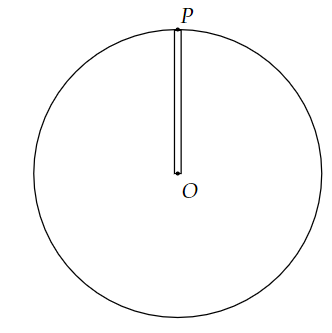
\includegraphics[width=0.31\textwidth]{imagens/q5(1).png}
            \caption{Esquema \(1\)}
        \end{figure}
        \switchcolumn
        \begin{figure}[h]
            \centering
            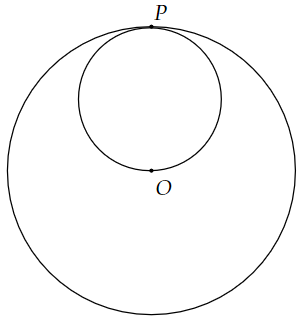
\includegraphics[width=0.3\textwidth]{imagens/q5(2).png}
            \caption{Esquema \(2\)}
        \end{figure}
    \end{paracol} 

    \begin{pssolution*}{}{}
        \begin{alternativas}
            \item A gravidade dentro de um planeta é dada por:
            \[\oint\mathbf{g}\cdot d\mathbf{S} = -4\pi GM_{int}\]
            \[4\pi r^2g = -4\pi G \rho \frac{4\pi}{3}r^3\]

            Ou seja, para o caso \(1\), \(g \propto -\rho r \rightarrow g = -k\rho r\). Utilizando a Segunda Lei de Newton:
            \[F = mv\frac{dv}{dr} = -mkr\]
            Integrando:
            \[\int_0^{v_1} v'dv' =-k\rho\int_0^R rdr\]

            \[\frac{v_1^2}{2} = k\rho\frac{R^2}{2} \rightarrow \boxed{v_1 = R \sqrt{k\rho}}\]

            Seja \(\mathbf{j}\) o vetor que parte do centro do planeta até o centro da cavidade. Utilizando superposição:
            \[a = -k\rho\mathbf{r} - k(-\rho)(\mathbf{r}-\mathbf{j}) = -k\rho\mathbf{j}\]
            Ou seja, no caso \(2\), a aceleração é constante e tem módulo \(|a| = \frac{k\rho R}{2}\).
            
            Utilizando Torricelli:
            \[v_2^2 = 2aR k\rho R^2 \rightarrow \boxed{v_2 = R\sqrt{k\rho}}\]
            Logo, \(v_1/v_2 = 1\).

            \item No primeiro caso, note que temos um M.H.S., uma vez que a força é proporcional a \(r\). O tempo até atingir a parte inferior seria igual a \(1/4\) do período:
            \[\ddot{r} = -k\rho r \rightarrow \omega^2 = k\rho \rightarrow T = \frac{2\pi}{\sqrt{k\rho}} \rightarrow t_1 = \frac{T}{4} = \frac{\pi}{2\sqrt{k\rho}}\]

            No segundo caso, temos uma aceleração constante, logo:
            \[t_2 = \frac{v_2}{a_2} = \frac{2R\sqrt{k\rho}}{k\rho R} = \frac{2}{\sqrt{k\rho}}\]

            Logo, a razão \(t_1/t_2\) é dada por:
            \[\boxed{\frac{t_1}{t_2} = \frac{\pi}{4}}\]

        \end{alternativas}
    \end{pssolution*}
\end{pproblem}

\pts{5}
\begin{pproblem} Calcular as velocidades de escape em certas situações pode ser mais complicado do que parece. Um exemplo disso é calcular a velocidade de lançamento que um foguete precisa ter para chegar a determinado local.
    \\
    \textbf{Dica:} Os problemas a seguir exigem que você pense cuidadosamente no referencial mais adequado. Não subestime a questão.
    \\
    \textbf{Dados:} Um corpo pode orbitar a superfície da Terra com velocidade \(v_0 = 7,9\text{ km/s}\), a velocidade orbital da Terra em torno do Sol é \(u_0 = 29,7\text{ km/s}\), e o raio da Terra é desprezível em relação à distância Terra-Sol. Considere também que, ao deixar o campo gravitacional da Terra, a distância entre a sonda e o Sol é a mesma distância entre a Terra e o Sol.
    \begin{enumerate}[label=\textbf{\alph*)}]
        \item Qual é a menor velocidade de lançamento que um foguete precisa ter para atingir o Sol, considerando que ele dê apenas um impulso? (Para conferir, \(v = 31,8\) km/s)
        \item Qual é a menor velocidade de lançamento que um foguete precisa ter para escapar do Sistema Solar? (Para conferir, \(v = 16,7\) km/s)
        \item Como a resposta do item \textbf{a)} muda se o foguete conseguir realizar um segundo impulso muito pequeno em algum ponto de sua órbita?
    \end{enumerate}

    \begin{pssolution*}{}{}
        \begin{alternativas}
            \item Para que isso aconteça, após deixar a Terra, no referencial do Sol, a sonda deve estar parada e, consequentemente, no referencial da Terra, ela deve estar com velocidade \(-u_0\). Utilizando conservação de energia:
            \[\frac{mv^2}{2}-\frac{GM_\oplus m}{R_\oplus} = \frac{mu_0^2}{2}\]
            \[v^2 = u_0^2+\frac{2GM_\oplus}{R_\oplus}\]

            Note que a velocidade \(v_0\) também pode ser obtida igualando a aceleração centrípeta com a gravitacional:
            \[\frac{mv_0^2}{R_\oplus} = \frac{GM_\oplus m}{R_\oplus^2} \rightarrow v_0^2 = \frac{GM_\oplus}{R_\oplus}\]

            Substituindo,

            \[v^2=u_0^2+2v_0^2 \rightarrow \boxed{v = 31,8\text{ km/s}}\]

            \item Nesse caso, ao sair do campo gravitacional da Terra, no referencial do Sol, o corpo deve ter uma velocidade \(\sqrt{2}u_0\), logo, no referencial da Terra, deve possuir \((\sqrt{2}-1)u_0\). Novamente, por conservação de energia:
            
            \[\frac{mv^2}{2}-\frac{GM_\oplus m}{R_\oplus} = \frac{m(\sqrt{2}-1)^2u_0^2}{2}\]

            \[v^2 = (\sqrt{2}-1)^2u_0^2+2v_0^2 \rightarrow \boxed{v = 16,7 \text{ km/s}}\]

            \item Imagine que façamos a sonda ir para o infinito, ou seja, a lançamos com velocidade \(v=16,7\text{ km/s}\), e, após isso, damos um impulso infinitesimal na direção do Sol. Isso faz com que a sonda percorra todo o caminho de volta e, consequentemente, atinja o Sol.
        \end{alternativas}
    \end{pssolution*}
\end{pproblem}

\pts{3} % problemas da semana 115
\begin{pproblem} (Kevin Zhou) A equação dos foguetes é dada por:
    \[
    v = u\ln\left(\frac{M_0}{M}\right)
    \]
    Onde \(v\) é a velocidade do foguete, \(u\) a velocidade relativa com que o foguete ejeta combustível, \(M_0\) a massa inicial do foguete e \(M\) sua massa atual.
    \begin{enumerate}[label=\textbf{\alph*)}]
        \item Deduza a equação dos foguetes partindo da conservação do momento.
        \item Considerando \(u\) um valor fixo durante todo o percurso do foguete, qual deve ser o valor de \(u\) para que o foguete vá de \(0\) até \(v\) gastando o menor combustível possível? (Você precisará resolver numericamente para \(v/u\))
        \item Como a equação dos foguetes deve ser corrigida para uma região do espaço com um campo gravitacional, \(\mathbf{g}\), constante e apontando na direção contrária ao movimento do foguete? Considere \(\eta = dm/dt = \text{constante}\).
    \end{enumerate}

    \begin{pssolution*}{}{}
        \begin{alternativas}
            \item Considere que o foguete possui massa \(M\) e velocidade \(v\). Ele ejeta combustível a uma velocidade relativa \(u\). Seja \(dm\) a massa de gás ejetada:
            \[dp = (v-u)dm\]
            Mas, pela definição,
            \[dp = vdm + mdv\]
            Combinando essas equações:
            \[mdv = -udm\]

            Integrando,
            \[\ln m = -\frac{v}{u} + C\]

            Sabemos que quando \(m = M_0\), temos \(v = 0\), então \(C = \ln M_0\). Assim:

            \[v = u \ln\left(\frac{M_0}{M}\right)\]

            Como esperado.

            \item A energia cinética do gás é dada por:
            
            \[K_{g} =\frac{1}{2}M_gu^2 = \frac{(M_0-M)u^2}{2}\]

            Podemos encontrar uma expressão para \(M\) utilizando a equação dos foguetes:

            \[\frac{M_0}{M} = e^{v/u} \rightarrow M_0 = Me^{v/u}\]

            Voltando à fórmula anterior:
            
            \[K_g = \frac{M(e^{v/u}-1)u^2}{2}\]

            Aqui, \(M\) seria o equivalente à massa da "carcaça" do foguete.

            Para minimizar a quantidade de energia gasta com combustível, temos:

            \[\frac{dK_g}{du}=0  \rightarrow -e^{v/u}v +2u(e^{v/u}-1)=0\]

            Definindo \(x=v/u\),

            \[e^xx = 2(e^x-1) \rightarrow x = 2(1-e^{-x})\]

            Resolvendo por iteração, encontramos:

            \[x \approx 1,59 \rightarrow \boxed{u \approx \frac{v}{1,59}} \]

            \item Nesse caso, temos:
            
            \[dp = (v-u)dm - mgdt = mdv +vdm\]
            \[\frac{dm}{m} = -\frac{dv}{u} - \frac{g}{u}dt\]

            Integrando,

            \[\ln\left(\frac{M}{M_0}\right) = -\frac{v}{u} - \frac{gt}{u}\]

            Como \(\eta\) é constante, \(M = M_0 -\eta t \rightarrow t = (M_0-M)/\eta\).

            \[\ln\left(\frac{M}{M_0}\right) = -\frac{v}{u} - \frac{g}{u\eta}(M_0-M)\]

            Resolvendo para \(v\),

            \[\boxed{v = u\ln\left(\frac{M_0}{M}\right)-\frac{g}{\eta}(M_0-M)}\]
        \end{alternativas}
    \end{pssolution*}
\end{pproblem}  

\pts{4}
\begin{pproblem} Um dos propelentes mais comuns em foguetes é uma mistura de hidrogênio líquido com oxigênio líquido. Quando começa a queimar, a seguinte reação química ocorre:
    \[
    2H_2 + O_2 \rightarrow 2H_2O
    \] 
    Para cada mol de hidrogênio, esta reação libera \(241,8 \text{ kJ}\) de energia. Ao longo da questão, suponha que toda essa energia seja utilizada para mover o foguete.
    \begin{enumerate}[label=\textbf{\alph*)}]
        \item Uma expedição espacial deseja ser feita de tal maneira que é necessário realizar uma transferência de Hohmann para lançar um foguete da Terra para Marte. Calcule a variação de velocidade total \(\Delta v\) necessária para realizar essa manobra.
        \item A partir do \(\Delta v\) calculado anteriormente, estime quantas toneladas de propelente devem ser utilizadas para realizar tal manobra para um foguete que ejeta propelente com velocidade \(u = 3,0\) km/s e carcaça com massa \(M = 140\cdot10^3\) kg.
    \end{enumerate}
    \begin{pssolution*}{}{}
        \begin{alternativas}
            \item Para o primeiro impulso, temos:
            \[v_{0,1}^2=\frac{GM}{R_T}\]
            \[v_{f,1}^2 = GM\left(\frac{2}{R_T}-\frac{1}{a}\right)\]
            A órbita de transferência possui \(a=(R_T+R_M)/2\),
            \[v_{f,1}^2 = \frac{2GM}{R_T}\left(\frac{R_M}{R_T+R_M}\right)\]

            Já no segundo impulso,
            \[v_{0,2}^2 = GM\left(\frac{2}{R_M}-\frac{1}{a}\right) = \frac{2GM}{R_M}\left(\frac{R_T}{R_T+R_M}\right)\]

            \[v_{f,2}^2 = \frac{GM}{R_M}\]

            Sendo \(\Delta v = \Delta v_1 + \Delta v_2 = (v_{f,1}-v_{0,1})+(v_{f,2}-v_{0,1})\), podemos equacionar:

            \[\boxed{\Delta v = \sqrt{\frac{2GM}{R_T}\left(\frac{R_M}{R_T+R_M}\right)}-\sqrt{\frac{GM}{R_T}} + \sqrt{\frac{GM}{R_M}} - \sqrt{\frac{2GM}{R_M}\left(\frac{R_T}{R_T+R_M}\right)}}\]
            
            Utilizando \(M = M_\odot = 2\cdot10^{30}\) kg, \(R_M = 1,5\) UA e \(R_T = 1\) UA, encontramos o valor numérico de \(\Delta v \approx 5,42 \) km/s.

            \item Utilizando a equação dos foguetes, temos:
            
            \[v = u\ln\left(\frac{M_0}{M}\right) \rightarrow \frac{M_0}{M}  = 1+ \frac{\mu}{M}= e^{v/u}\]

            Onde \(\mu\) é a massa de gás.

            \[\boxed{\mu = M(e^{v/u}-1) \approx 7,12 \cdot 10^5 \text{ kg}}\]

            O que é condizente com a realidade, uma vez que a massa do combustível é \(\approx 83\%\) da massa total do foguete.
        \end{alternativas}
    \end{pssolution*}
\end{pproblem}

\pts{3} % problemas da semana 115
\begin{pproblem} Marisso estava estudando um sistema binário com inclinação \(i\). Ele conseguiu descobrir que o maior redshift vindo da estrela \(1\) era \(z_1\). Sabendo disso, ache uma expressão para a massa da estrela \(2\), \(m_2\), deixe sua resposta em função de \(z_1\), do período do binário \(P\), da inclinação \(i\), da razão entre as massas \(\lambda  = m_2/m_1\) e de constantes fundamentais.
    \begin{pssolution*}{}{}
        A velocidade com que \(1\) orbita o CM é:

        \[v_1 = \frac{2\pi a_1}{P}\]

        Pela geometria, a velocidade radial é \(v_{r,1}=v_1\sin i\), com isso:

        \[z_1 \approx \frac{v_{r,1}}{c} = \frac{2\pi a_1\sin i}{Pc}\]

        Do teorema do centro de massa:

        \[m_1a_1=m_2a_2 \rightarrow a_2 = \frac{a_1}{\lambda}\]

        Utilizando a terceira Lei de Kepler:

        \[\frac{(a_1+a_2)^3}{P^2} = \frac{G(m_1+m_2)}{4\pi^2}\]

        \[\frac{a_1^3(1+1/\lambda)^3}{P^2} = \frac{Gm_2(1+1/\lambda)}{4\pi^2}\]

        Isolando \(m_2\):

        \[m_2 = \frac{4\pi^2a_1^3(1+1/\lambda)^2}{GP^2}\]

        \(a_1\) pode ser obtido avaliando a fórmula do redshift, \(a_1 = Pcz_1/2\pi\sin i\):

        \[m_2 = \frac{4\pi^2}{GP^2}\left(\frac{z_1Pc}{2\pi\sin i}\right)^3(1+1/\lambda)^2\]

        Por fim, simplificando:

        \[\boxed{m_2 = \frac{z_1^3c^3P}{2\pi G \sin^3i}(1+1/\lambda)^2}\]
    \end{pssolution*}
\end{pproblem}

\pts{2}
\begin{pproblem} Qual é a razão entre \(a)\) as forças gravitacionais causadas pelo Sol e pela Lua na superfície da Terra? E \(b)\) das forças de maré causadas pelo mesmo?
    \begin{pssolution*}{}{}
        \begin{alternativas}
            \item A força gravitacional tem a forma:
            \[F_G = \frac{GMm}{d^2}\]

            Assim,

            \[\frac{F_\odot}{F_L} = \frac{M_\odot}{M_L}\left(\frac{d_{T-L}}{d_{T-\odot}}\right)^2 \boxed{\approx 178,33}\]

            \item Para as forças de maré, temos:
            
            \[F_M \propto \frac{m}{d^3}\]

            \[\therefore \frac{F_\odot}{F_L} = \frac{M_\odot}{M_L}\left(\frac{d_{T-L}}{d_{T-\odot}}\right)^3 \boxed{\approx 0,456}\]

        \end{alternativas}
    \end{pssolution*}
\end{pproblem}

\pts{4}
\begin{pproblem} (Morin 7.7) Uma partícula de massa \(m\) viaja em uma órbita hiperbólica com uma massa \(M\) fixa em um dos focos. A velocidade no infinito é \(v_0\) e o parâmetro de impacto é \(b\).
    \begin{alternativas}
    \item Mostre que o ângulo de desvio da partícula é dado por:
    \[
    \phi = \pi-2\tan^{-1}(\gamma b)
    \]
    Onde \(\gamma \equiv v_0^2/GM\).
    \item Sendo \(d\sigma\) a seção transversal da partícula (medida quando a mesma se encontra no infinito) que é defletida em um ângulo sólido de tamanho \(d\Omega\). Mostre que:
    \[
    \frac{d\sigma}{d\Omega} = \frac{1}{4\gamma^2\sin^4(\phi/2)}
    \] 
    A título de curiosidade, essa quantidade é chamada de \textit{seção transversal diferencial}.
    \end{alternativas}

    \begin{pssolution*}{}{}
        \begin{alternativas}
            \item O esquema da situação é o seguinte:
            
            \begin{figure}[H]
                \centering
                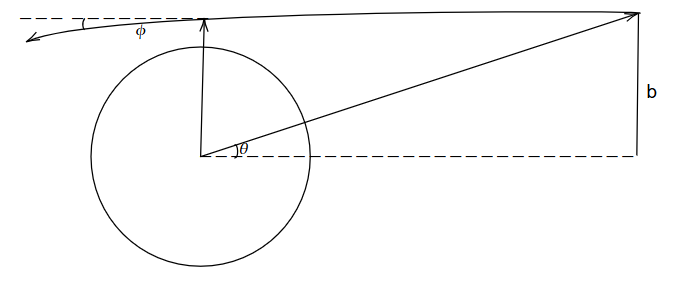
\includegraphics[width=0.87\linewidth]{imagens/orbita hiperbolica esquema 1.png}
                \caption{Esquema da Órbita Hiperbólica}
                \label{fig.1}
            \end{figure}

            Para achar o ângulo de desvio \(\phi\), vamos usar o teorema do Impulso, considerando as componentes horizontais e verticais da força de atração:

            \[F_x = -\frac{GMm}{r^2}\cos\theta, \ \ F_y = -\frac{GMm}{r^2}\sin\theta\]

            O teorema do Impulso nos diz que:
            \[\int F_i dt = \Delta p\]

            Onde \(p_i\) é o momento da partícula na direção \(i\).

            No eixo \(x\), temos:

            \[-\int \frac{GMm}{r^2}\cos\theta dt = \Delta p_x \]

            Note que integrar com relação ao tempo deixa as coisas inconvenientes, pois descobrir como \(\theta\) e \(r\) variam no tempo é algo complicado. Por isso, vamos recorrer à definição de momento angular. Utilizando que \(L = mr^2d\theta/dt\), temos:

            \[dt = \frac{mr^2}{L}d\theta\]

            Substituindo esse valor na nossa integral:
            \[-\int \frac{GMm^2}{L}\cos\theta d\theta = \Delta p_x\]

            Perceba que nossa integral vai de \(\theta = 0\), situação no infinito, até \(\theta = \pi - \phi\), situação no infinito após o desvio. Assim:

            \[-\frac{GMm^2}{L}\int_0^{\pi-\phi}\cos\theta d\theta = -\frac{GMm^2}{L}\sin\theta\big|_0^{\pi-\phi} = -\frac{GMm^2}{L}\sin(\pi-\phi) = \Delta p_x\]

            Analogamente para \(y\):

            \[-\frac{GMm^2}{L}\int_0^{\pi-\phi}\sin\theta d\theta = \Delta p_y\]
            \[=\frac{GMm^2}{L}\cos\theta\big|_0^{\pi-\phi} \equiv -\frac{GMm^2}{L}(1-\cos(\pi-\phi)) = \Delta p_y\]
        
            Note também que \(\Delta p_x = m(v_{f,x}-v_0), \ \Delta p_y = m(v_{f,y}-0)\). Podemos achar também uma relação de \(\phi\) com as velocidades e, por pura geometria, obtemos:
            \[\tan\phi =-\frac{v_{f,y}}{v_{f,x}}\]
            Como só há forças centrais, \(L\) é um valor constante, e da situação inicial, o mesmo vale \(L = mbv_0\). Agora, indo para as contas:

            \[-\frac{GM}{bv_0}\sin(\pi-\phi) = v_{f,x}-v_0, \ \ -\frac{GM}{bv_0}(1-\cos(\pi-\phi))=v_y\]
            
            Com essas duas equações, obtemos:

            \[\frac{v_{f,y}}{v_{f_x}}= -\frac{GM(1-\cos(\pi-\phi))}{bv_0^2-GM\sin(\pi-\phi)}\]

            Ou seja:

            \[\tan\phi = \frac{GM(1-\cos(\pi-\phi))}{bv_0^2-GM\sin(\pi-\phi)}\]

            Resolvendo para \(\phi\), obtemos o resultado esperado. Uma outra maneira de realizar a mesma questão é pensar puramente na geometria da situação:
            \begin{figure}[H]
                \centering
                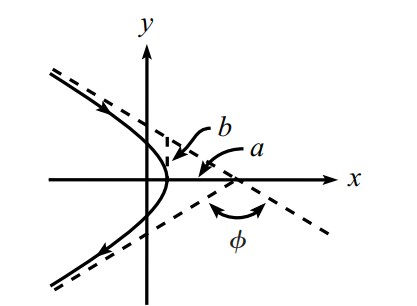
\includegraphics[width=0.7\linewidth]{imagens/morin hiperbole.png}
                \caption{Fonte: Morin 7.7}
            \end{figure}

            Aqui, é evidente que:

            \[\phi = \pi - 2\tan^{-1}\left(\frac{b}{a}\right)\]

            Onde \(b\) é o parâmetro de impacto e \(a\) o semi-eixo da hipérbole. Do conhecimento de cônicas, temos:
            \[\frac{b}{a} = \sqrt{e^2-1} = \sqrt\frac{2EL^2}{m(GMm)^2} = \frac{v_0^2b}{GM} \equiv \gamma b\]

            Em ambas as maneiras, chegamos no mesmo resultado:

            \[\boxed{\phi = \pi - \tan^{-1}(\gamma b)}\]

            Como desejado.

            \item Considere um anel de espessura \(db\) e raio \(b\). Agora, considere uma esfera bem grande, com centro em \(M\). Qualquer partícula que passar pela seção transversal do anel de raio \(b\) irá atingir essa esfera fazendo um ângulo \(\phi\) com o eixo \(x\), com uma separação angular \(d\phi\). Usando que \(d\cot x/dx = -1/\sin^2x\), temos:
            
            \[\big|\frac{db}{d\phi}\big| = \frac{1}{2\gamma \sin^2(\phi/2)}\]

            A área de seção transversal é dada por \(d\sigma = 2\pi bdb\) e o ângulo sólido de uma esfera é dado por \(d\Omega = 2\pi \sin\phi d\phi\). Portanto:

            \[\frac{d\sigma}{d\Omega} = \frac{2\pi b}{2\pi \sin \phi}\frac{db}{d\phi} = \left(\frac{(1/\gamma)\cot(\phi/2)}{2\sin(\phi/2)\cos(\phi/2)}\right)\left(\frac{1}{2\gamma\sin^2(\phi/2)}\right)\]

            \[\boxed{\frac{d\sigma}{d\Omega} = \frac{1}{4\gamma^2\sin^4(\phi/2)}}\]
        \end{alternativas}            
    \end{pssolution*}
\end{pproblem}

\begin{psidea}{}{}
    Em certas questões, é válida a utilização de vetores. Um exemplo é a questão abaixo. Para facilitar, na parte de encontrar a inclinação da órbita, observe a seguinte imagem:

    \begin{figure}[H]
        \centering
        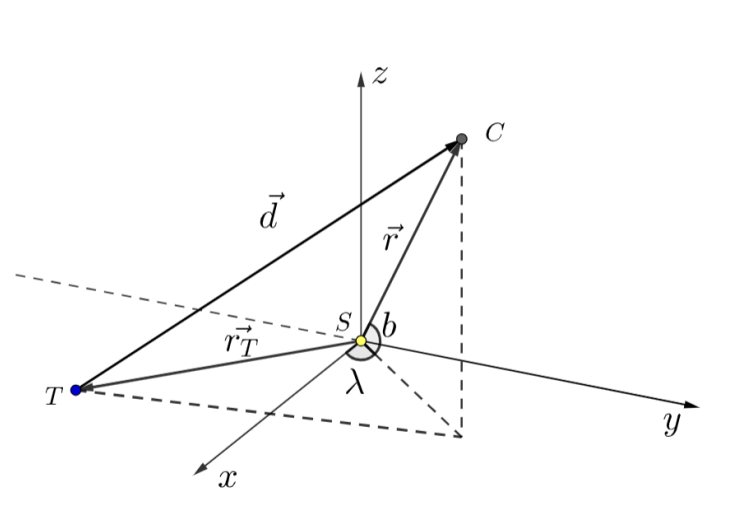
\includegraphics[width=0.7\linewidth]{imagens/vetores ecliptica.png}
        \caption{Vetores}
    \end{figure}

    Aqui, \(C\) representa um corpo, \(T\) a Terra e \(S\) o Sol. Os ângulos \(\lambda\) e \(b\) denotam, respectivamente, a longitude e a latitude eclíptica. \(\vec{r}\) é o vetor entre o Sol e o corpo, \(\vec{r}_T\) o vetor entre o Sol e a Terra, e \(\vec{d}\) o vetor entre a Terra e o corpo.
    Pela figura,

    \[\vec{r} = r(\cos b\cos\lambda \hat{x}+ \cos b \sin\lambda \hat{y} + \sin b \hat{z})\]

    \[\vec{r}_T = r_T(\cos(\omega_\oplus t)\hat{x}+\sin(\omega_\oplus t)\hat{y})\]

    Assim, \(\vec{d}=\vec{r}-\vec{r}_T\):

    \[
    \vec{d} = \big(r \cos b \cos \lambda - r_T \cos (\omega_\oplus t)\big) \hat{x} 
    + \big(r \cos b \sin \lambda - r_T \sin (\omega_\oplus t)\big) \hat{y} 
    + r \sin b \, \hat{z}
    \]

    Calculando o módulo do vetor \(\vec{d}\), obtemos que:

    \[
    d = |\vec{d}| = \sqrt{r_T^2 + r^2 - 2 r_T r \cos b \cos (\lambda - \omega_\oplus t)}
    \]

    Portanto:

    \[
    \boxed{\cos b \cos (\lambda - \omega_\oplus t) = \frac{r_T^2 + r^2 - d^2}{2 r_T r}}
    \]
\end{psidea}

\pts{5}
\begin{pproblem}(Lista \(1\) - Vinhedo 2024) 
    CR4b-2023 é uma sonda em órbita heliocêntrica que foi construída e lançada em 2023 pelo jovem prodígio Caranguejo. O objetivo da sonda era estudar as tempestades solares e captar dados para que Caranguejo analisasse em seu observatório no Espírito Santo. CR4b-2023, porém, durante uma de suas expedições ao Sol, foi atingida por uma tempestade solar e sofreu uma danificação grave. Devido a isso, a sonda se desorientou e, assim, teve todos os seus parâmetros orbitais alterados, de maneira que Caranguejo não soubesse mais sua localização.

    Visando rastrear a posição de CR4b-2023 novamente, Caranguejo utilizou-se de seu observatório para coletar os valores das separações angulares \(\Delta\phi\) entre a sonda e o Sol e os valores do diâmetro angular \(\theta_S\) da sonda, tudo em função do tempo \(t\). A tabela obtida por Caranguejo pode ser vista abaixo.

    \begin{table}[H]
        \centering
        \begin{tabular}{|c|c|c|}
            \hline
            \(\Delta\phi\) (Graus) & \(\theta_S\) (mas) & \(t\) (Dias) \\
            \hline
            0,000 & 99,27 & 0,00 \\
            4,889 & 103,67 & 1,79 \\
            17,354 & 104,72 & 7,43 \\
            29,015 & 93,06 & 20,62 \\
            27,793 & 81,18 & 25,41 \\
            13,460 & 79,77 & 45,98 \\
            11,539 & 77,97 & 51,61 \\
            2,466 & 76,44 & 54,53 \\
            2,656 & 74,84 & 55,31 \\
            7,177 & 73,90 & 57,19 \\
            10,800 & 70,63 & 58,43 \\
            22,464 & 72,92 & 91,67 \\
            13,823 & 80,50 & 130,48 \\
            \hline
        \end{tabular}
        \caption{Valores medidos por Caranguejo}
    \end{table}

    Considere que, no momento inicial \(t_0 = 0\) em que a sonda é atingida pela tempestade solar, o Sol estava exatamente no ponto de Libra e o movimento da sonda era ascendente em relação ao plano da eclíptica. Além disso, considere que o raio da sonda, supostamente esférica, é dado por \(R = 30\) km. Para essa questão, não é necessário fazer análise de erros (apesar de ser importante tentar utilizar métodos visando diminuir erros estatísticos). Com base no que foi apresentado:

    \begin{enumerate}[label=(\alph*)]
        \item Calcule os parâmetros orbitais da órbita de CR4b-2023, ou seja, seu semi-eixo maior \(a\), excentricidade \(e\), inclinação \(i\), longitude do nodo ascendente \(\Omega\) e argumento do periélio \(\omega\). Como em todas as questões de análise de dados, você deve fornecer tabelas de dados claramente rotuladas, gráficos claramente rotulados e derivações de fórmulas suficientes para deixar claro o que você mediu e como está derivando seus resultados visando reduzir erros estatísticos.
        
        \item Considerando \((x', y', z')\) como as coordenadas de CR4b-2023 em um sistema cartesiano de mão direita em que o plano \(x'y'\) se localiza no plano da órbita da sonda, o Sol se localiza na origem, e o eixo \(x'\) aponta para o ponto vernal, escreva, em uma tabela, os valores de pelo menos 5 pontos \((x', y', z')\) distintos. Com base nos dados encontrados, esboce, em um gráfico, a órbita de CR4b-2023, indicando as coordenadas de seu centro.
        
        \item Considerando agora um novo sistema de coordenadas de mão direita \((x, y, z)\), no qual o Sol se localiza na origem, o plano \(xy\) representa o plano da eclíptica, e o eixo \(x\) aponta para o ponto vernal, escreva as coordenadas do centro da órbita de CR4b-2023. Por fim, calcule a distância \(d_{TC}\) entre o centro da órbita terrestre e o centro da órbita da sonda.
    \end{enumerate}

    \begin{pssolution*}{}{}
        \begin{alternativas}
            \item A ideia dessa parte da questão é encontrar uma relação entre os dias e a distância da sonda até o Sol. Utilizando trigonometria básica, podemos dizer que a distância da sonda até a Terra é dada por:
            \[d_{S-\oplus} = R/\tan^{-1}\left(\frac{\theta_S}{2}\right)\]
            Onde \(R\) é o raio da sonda.
            Aqui, podemos utilizar a lei dos cossenos para encontrar a relação dessa distância com a distância da sonda até o Sol. Considerando a órbita da Terra circular de raio \(d_{\odot-\oplus}\) e definindo por \(d\) a distância entre a sonda e o Sol, temos:
            \[d^2 = d_{\odot-\oplus}^2+d_{S-\oplus}^2-2d_{\odot-\oplus}d_{S-\oplus}\cos\Delta\phi\]      
            
            Com isso, podemos montar a seguinte tabela, com os valores de \(d\) em UA e os valores de \(t\) em dias.

            \[
                \begin{array}{|c|c|}
                \hline
                \text{t (Dias)} & \text{d (UA)} \\
                \hline
                0.00 &    0.17 \\
                1.79 &    0.22 \\
                7.43 &    0.34 \\
                20.62 &    0.50 \\
                25.41 &    0.49 \\
                45.98 &    0.24 \\
                51.61 &    0.22 \\
                54.53 &    0.09 \\
                55.31 &    0.12 \\
                57.19 &    0.18 \\
                58.43 &    0.27 \\
                91.67 &    0.44 \\
                130.48 &    0.25 \\
                \hline
                \end{array}
            \]

            Plotando um gráfico de \(t\) por \(d\), temos:
            
            \begin{figure}[H]
                \centering
                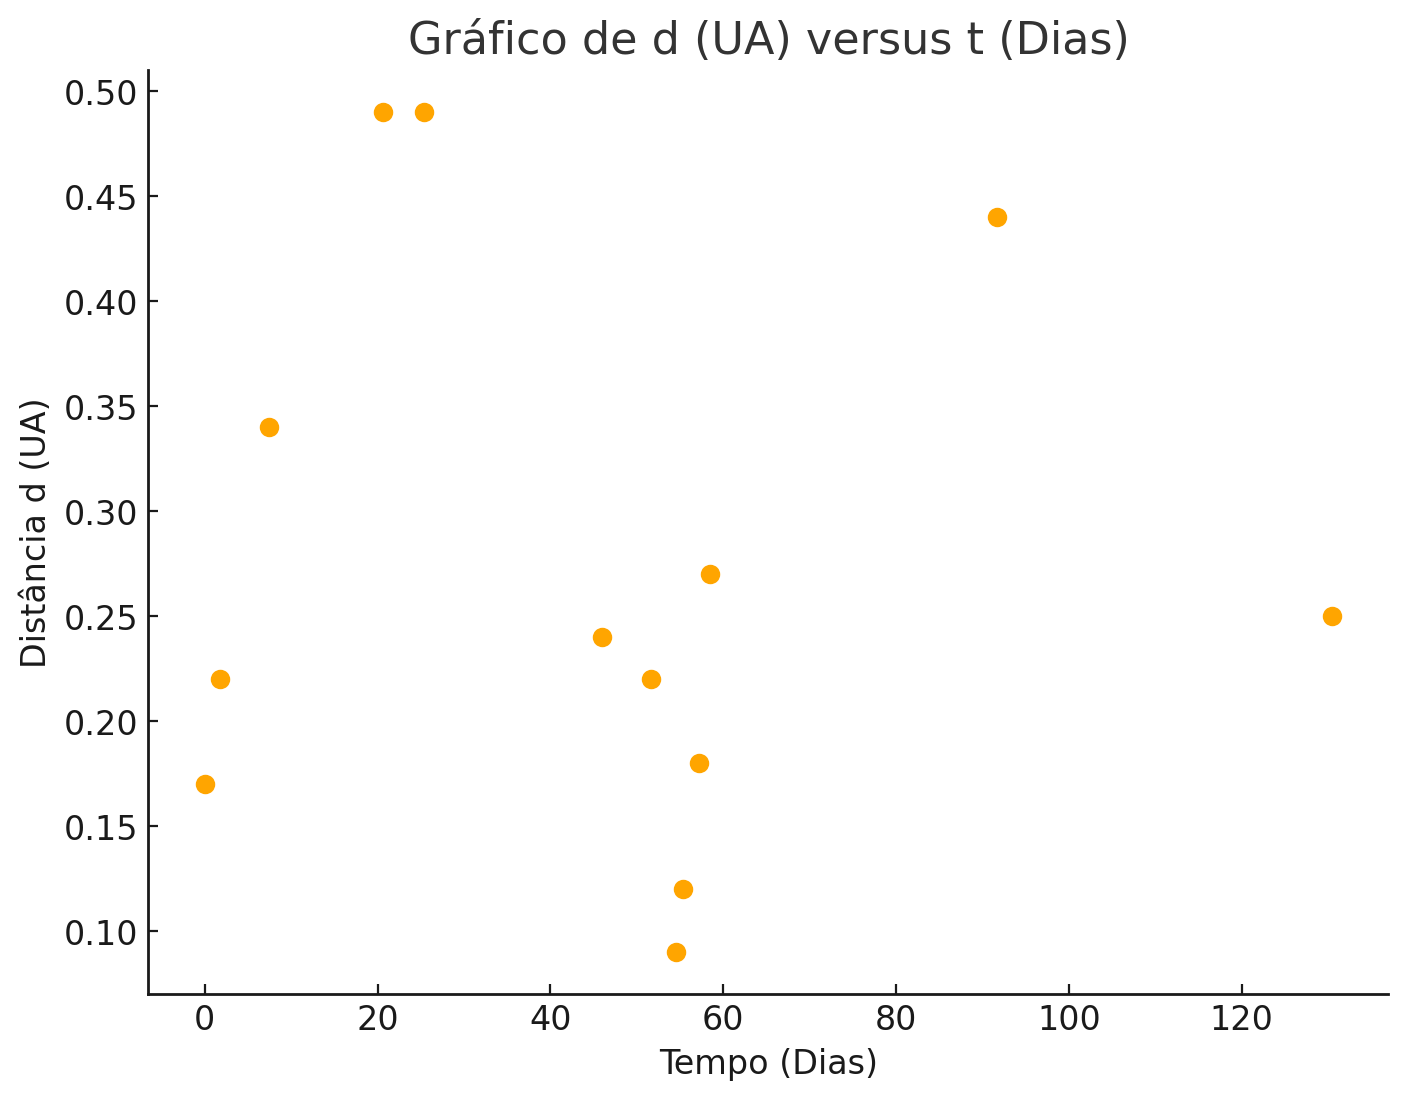
\includegraphics[width=0.85\linewidth]{imagens/graficoorbita.png}
            \end{figure}

            Agora, vamos colocar a mão na massa e achar os parâmetros requisitados: semi-eixo maior, \(a\), excentricidade, \(e\), inclinação, \(i\), longitude do nodo ascendente \(\Omega\) e argumento do periélio, \(\omega\). Os dois primeiros podem ser obtidos diretamente dos dados que analisamos até o momento.

            Analisando os dados, podemos perceber que a menor distância entre a sonda e o Sol é dada por \(a_p = 0.09\) UA e a maior distância é dada por \(a_a = 0,49\) UA. Essas distâncias devem corresponder ao periélio e ao afélio, respectivamente. Utilizando a definição:
            \[a_p = a(1-e), \ a_a=a(1+e) \rightarrow \frac{a_p}{a_a}=\frac{1-e}{1+e} \approx 0,18\]
            
            Resolvendo, obtemos \(e \approx 0,67\).

            Usando que \(a = \frac{a_p+a_a}{2}\), obtemos \(a\approx 0,30\) UA.

            Para acharmos os fatores angulares, temos que pensar um pouco mais. Começando por \(\Omega\), note que no momento inicial, em \(t=0\), a separação angular entre o Sol e a sonda é \(\Delta \phi = 0\). O enunciado nos diz que nesse momento o Sol se encontra no ponto de Libra, assim, temos que a sonda também se encontra no ponto de Libra e, como seu movimento era ascendente, temos \(\Omega = 0^\circ\).

            Para encontrar \(\omega\) e \(i\), vamos nos atentar ao seguinte triângulo esférico:

            \begin{figure}[H]
                \centering
                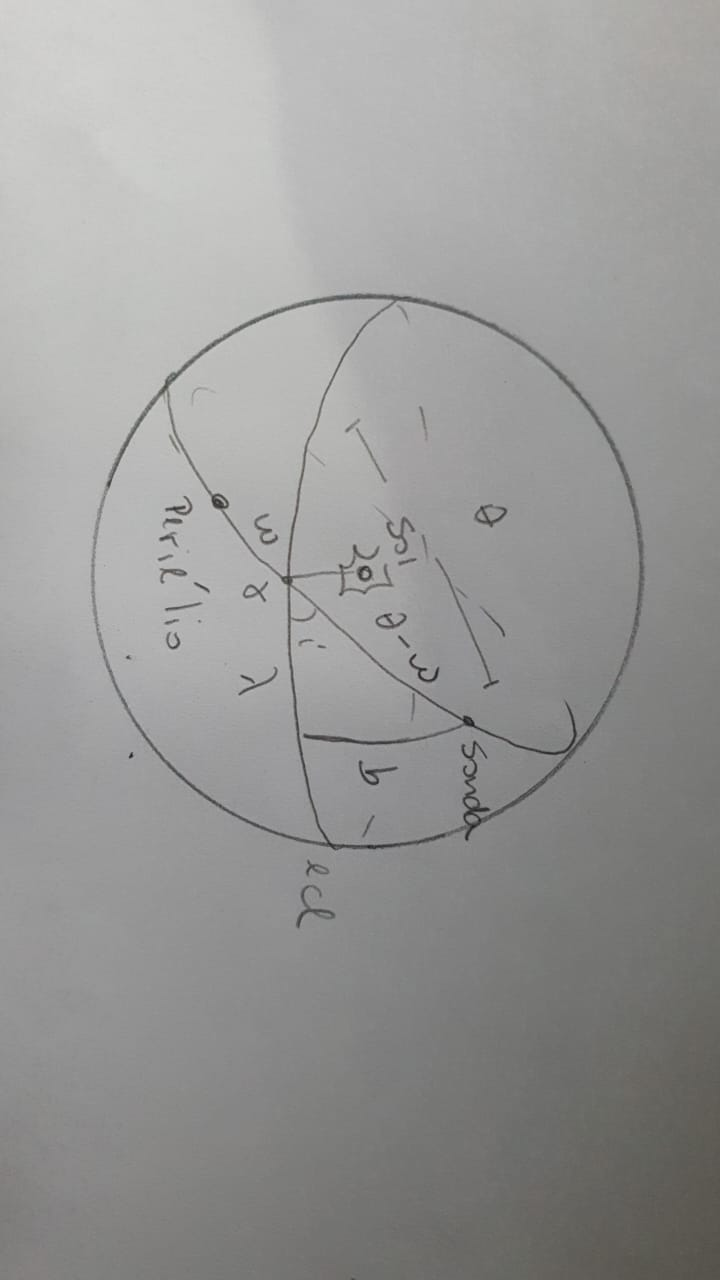
\includegraphics[angle=90, width=0.8\textwidth]{imagens/trigesfericoorbita.jpg}
                \caption{Esquema}
            \end{figure}

            Da forma polar da elipse, \(r=\frac{a(1-e^2)}{1+e\cos\theta}\), onde \(\theta\) é a anomalia verdadeira da órbita, podemos encontrar \(\omega\). Perceba que no instante inicial, \(t=0\), a sonda está exatamente no ponto de Libra, assim \(\theta = 2\pi-\omega\) conforme o esquema.

            Assim, temos:

            \[d(0) = \frac{a(1-e^2)}{1+e\cos(2\pi-\omega)}\]

            Resolvendo para \(\omega\):

            \[\omega = 2\pi-\cos^{-1}\left(\frac{a(1-e^2)}{d(0)e}-\frac{1}{e}\right) \approx 267,6^\circ \approx 270^\circ\]

            Substituindo os valores encontrados.

            Para achar a inclinação, vamos utilizar a lei dos cossenos:

            \[\cos(\theta-\omega)=\cos\lambda\cos b + \sin\lambda\sin b\cos(\pi/2) = \cos\lambda\cos b\]
            
            Note que \(\cos(\theta-\omega) \approx \cos(\theta-270^\circ) = \sin \theta\).

            Reescrevendo,

            \[\cos b = \frac{\sin\theta}{\cos\lambda}\]

            Utilizando a relação obtida na ideia anterior,

            \[\cos b  = \frac{r_T^2 + r^2 - d^2}{2 r_T r\cos (\lambda - \omega_\oplus t)}\]

            Igualando essas expressões e resolvendo para \(\lambda\),

            \[\lambda = \tan^{-1} \left( 
                \frac{r_T^2 + r^2 - d^2}{2 r_T r \sin \theta \sin (\omega_\oplus t)} - \cot (\omega_\oplus t)
                \right)\]

            Onde:

            \[
            \theta = \arccos \left( \frac{a (1 - e^2)}{e r} - \frac{1}{e} \right)
            \] 
            
            Com isso, podemos fazer a seguinte tabela, com os valores de \(b\) e \(\lambda\).

            \[
            \begin{array}{|c|c|}
            \hline
            \lambda \, (\text{Graus}) & b \, (\text{Graus}) \\ \hline
            0,000     & 0,00     \\ 
            17,495    & 9,847    \\ 
            45,905    & 22,521   \\ 
            78,492    & 29,499   \\ 
            101,508   & 29,499   \\ 
            134,095   & 22,521   \\ 
            163,504   & 9,847    \\ 
            180,000   & 0,000    \\ 
            197,495   & -9,847   \\ 
            216,005   & -18,747  \\ 
            270       & -30      \\ 
            333,435   & -14,478  \\ 
            17,495    & 9,847    \\ 
            78,492    & 29,499   \\ 
            143,994   & 18,747   \\ \hline
            \end{array}
            \]

            Voltando ao triângulo esférico e utilizando a lei dos quatro elementos, temos:

            \[\cos\lambda\cos90^\circ = \sin\lambda\cot b -\sin90^\circ\cot i\]

            Simplificando:

            \[\tan b = \tan i \sin \lambda\]

            Note que isso se assemelha a uma função do tipo \(y= A + Bx\). Fazendo uma regressão linear na calculadora, encontramos \(B\approx 0,578\). De modo que \(\tan i = B\), chegamos em:

            \[\boxed{i \approx 30^\circ}\]

        \item Como o Sol se localiza na origem, os valores de \(x'\) e \(y'\) podem ser calculados por:
            \[
            x' = r \sin \theta
            \]
            e
            \[
            y' = -r \cos \theta
            \]

            Escrevendo em uma tabela cinco valores diferentes de \(x'\) e \(y'\), obtemos que:

            \[
            \text{Tabela 7: Valores de \(x'\) e \(y'\)}
            \]

            \[
            \begin{array}{|c|c|}
            \hline
            x'\text{ UA} & y'\text{ UA} \\ \hline
            0,167 & 0,000 \\ \hline
            0,084 & 0,478 \\ \hline
            -0,219 & 0,261 \\ \hline
            -0,203 & 0,074 \\ \hline
            0,000 & -0,100 \\ \hline
            \end{array}
            \]

            Perceba que quaisquer valores, desde que corretos, de \(x'\) e \(y'\) podem ser utilizados. Além do mais, é importante aumentar o espaçamento entre os valores de \(x'\) e \(y'\) visando diminuir os erros associados ao esboço da órbita. Com base nisso, podemos plotar o gráfico:

            \begin{figure}[H]
                \centering
                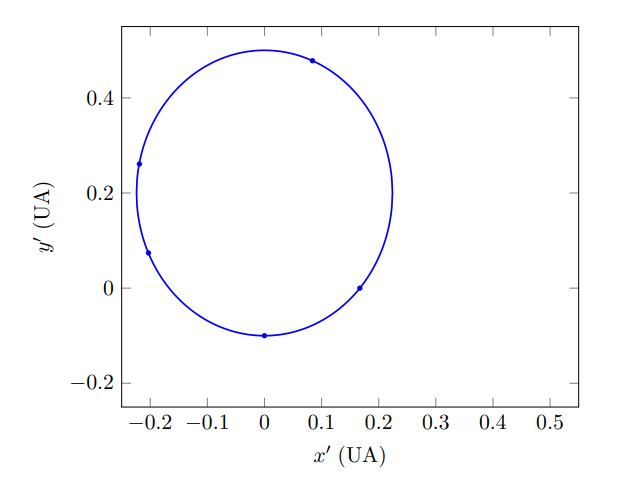
\includegraphics[width=0.7\linewidth]{imagens/graforbt.png}  
                \caption{Gráfico da órbita} 
            \end{figure}

            Observando o gráfico, vemos que as coordenadas \((x', y', z')\) do centro da elipse são \(\boxed{(0;\ 0,2; \ 0)}\).

        \item Aqui, vamos utilizar uma matriz de rotação em torno do eixo \(x\), dada por:
        
            \[
            \begin{pmatrix}
            x \\
            y \\
            z
            \end{pmatrix}
            =
            \begin{pmatrix}
            1 & 0 & 0 \\
            0 & \cos \alpha & \sin \alpha \\
            0 & -\sin \alpha & \cos \alpha
            \end{pmatrix}
            \begin{pmatrix}
            x' \\
            y' \\
            z'
            \end{pmatrix}
            \] 

            Para \(\alpha=i=30^\circ\):

            \[
            \begin{pmatrix}
            x \\
            y \\
            z
            \end{pmatrix}
            =
            \begin{pmatrix}
            1 & 0 & 0 \\
            0 & \cos 30^\circ & \sin 30^\circ \\
            0 & -\sin 30^\circ & \cos 30^\circ
            \end{pmatrix}
            \begin{pmatrix}
            x' \\
            y' \\
            z'
            \end{pmatrix}
            \]

            Então:
            \[
            x = x'
            \]
            \[
            y = y' \cos 30^\circ + z' \sin 30^\circ
            \]
            \[
            z = -y' \sin 30^\circ + z' \cos 30^\circ
            \]

            Substituindo os valores numéricos, obtemos que as coordenadas \((x, y, z)\) do centro de CR4b-2023 são dadas por:
            \[
            (0.000, 0.173, -0.100).
            \]

            Por fim, obtemos então que a distância entre o centro da órbita terrestre e o centro da órbita da sonda é dada por:
            \[
            d = \sqrt{\lvert x^2 + y^2 + z^2 \rvert}
            \]

            ou seja:
            \[
            \boxed{d = 0.200 \, \text{UA}}
            \]
        \end{alternativas}
    \end{pssolution*}
\end{pproblem}

\pts{5}
\begin{pproblem} (Iran Problem Set) 
    Uma partícula de massa \(m\) está orbitando um objeto massivo de massa \(M\). Mostre que o impulso necessário para fazer a órbita girar um ângulo \(\eta\) em torno de um dos focos é dado por:
    \[
    \Delta v = \frac{2\mu e}{h}\sin\left(\frac{\eta}{2}\right),
    \]
    onde:
    \begin{itemize}
        \item \(h\) é o momento angular por unidade de massa;
        \item \(\mu = GM\), sendo \(G\) a constante gravitacional.
    \end{itemize}
    \begin{pssolution*}{}{}
        Desenhando a órbita e a órbita rotacionada:

        \begin{figure}[H]
            \centering
            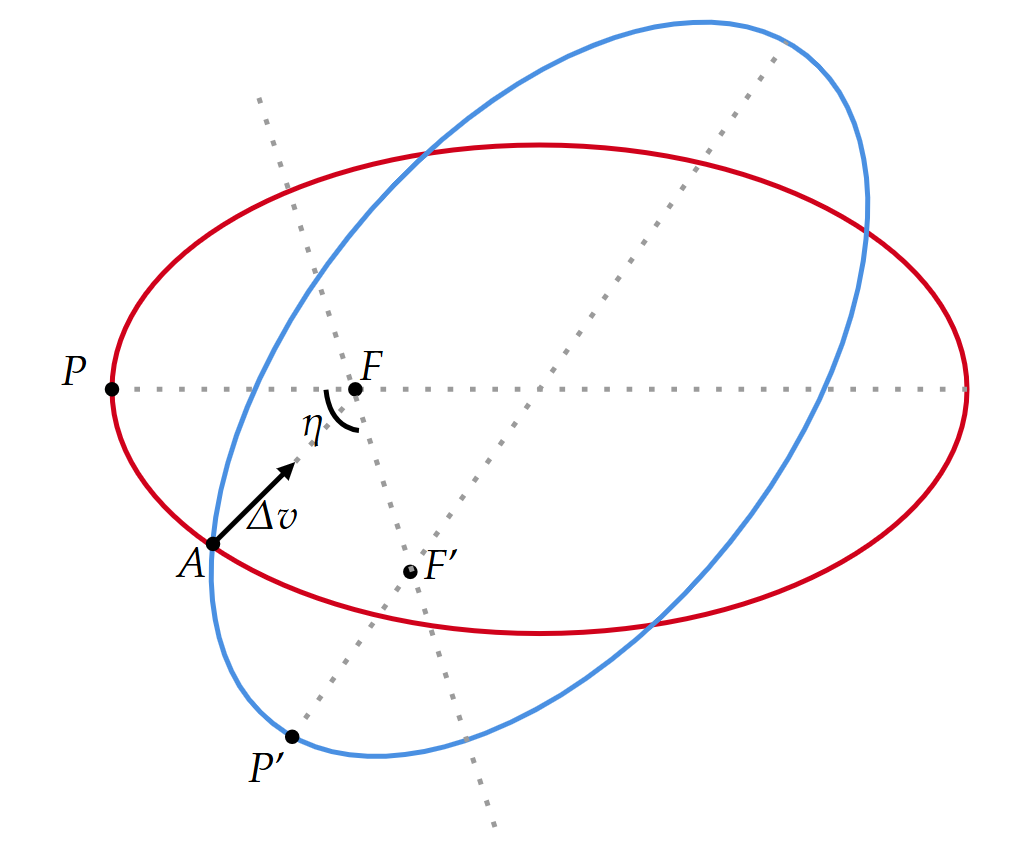
\includegraphics[width=0.7\linewidth]{imagens/esquemarotorb.png}
            \caption{Esquema da órbita rotacionada.}
        \end{figure}

        Perceba que o impulso só pode ser realizado nos pontos de interseção das duas órbitas e deve ser radial, uma vez que o momento angular deve continuar constante, a fim de manter a órbita idêntica. Vamos definir por \(X\) um ponto na órbita antes do impulso e \(X'\) um ponto na órbita após a rotação.

        Vamos às seguintes definições: \(F\) é o foco, \(P\) é o periélio da órbita, e \(A\) é o ponto de interseção onde é realizado o impulso.

        Por simetria, note que os ângulos \(AFP\) e \(AFF'\) são iguais e, portanto, têm valor \(\eta/2\).

        Como as duas órbitas possuem o mesmo momento angular, a velocidade tangencial no ponto \(A\) deve ser equivalente para ambas as órbitas. Além disso, podemos perceber que o ponto \(A\) possui anomalia verdadeira \(\theta = \eta/2\), o que garante que o módulo da velocidade também seja o mesmo para ambas as órbitas.

        \begin{figure}[H]
            \centering
            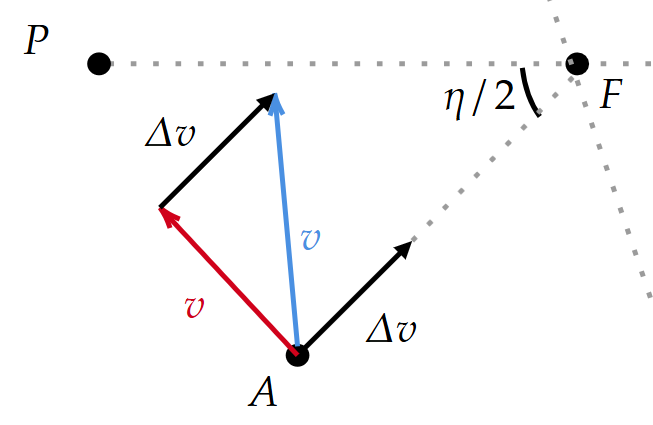
\includegraphics[width=0.7\linewidth]{imagens/rotorbt1.png}
            \caption{Vetores de velocidade.}
        \end{figure}

        A única maneira de isso ser possível seria se o impulso radial fosse dado por \(\Delta v = 2v_r\), onde \(v_r\) é a velocidade radial imediatamente antes do impulso.

        É claro que \(v_r^2 = v^2 - v_t^2\), onde \(v_t\) é a velocidade tangencial. Partindo de definições básicas:

        \[
        h^2 = \mu a (1 - e^2), \quad r = \frac{a(1 - e^2)}{1 - e\cos\theta}, \quad v_t = \frac{h}{r}, \quad v^2 = \mu \left(\frac{2}{r} - \frac{1}{a}\right).
        \]

        Trabalhando com essas equações, chegamos a:

        \[
        v^2 = \frac{\mu^2}{h^2}(1 + 2e\cos\theta + e^2), \quad v_t^2 = \frac{\mu^2}{h^2}(1 + e\cos\theta)^2.
        \]

        Por fim, substituindo em \(v_r^2 = v^2 - v_t^2\), obtemos:

        \[
        v_r^2 = \frac{\mu^2}{h^2}(e^2 - e^2\cos^2\theta) \equiv \frac{\mu^2e^2}{h^2}\sin^2\theta.
        \]

        Substituindo \(\Delta v = 2v_r\) e \(\theta = \eta/2\), chegamos ao resultado desejado:

        \[
        \boxed{\Delta v = \frac{2\mu e}{h}\sin\left(\frac{\eta}{2}\right) \blacksquare}
        \]
    \end{pssolution*}
\end{pproblem}


\pts{3}
\begin{pproblem}
    Nessa questão, vamos estudar um modelo simplificado para o efeito que confirmou a Teoria da Relatividade Geral de Einstein: as lentes gravitacionais. A presença de um corpo massivo curva o espaço-tempo, fazendo com que estrelas possam servir como lentes no espaço. Alguns telescópios, como o JWST, utilizam esse efeito para conseguir fotografar aglomerados de galáxias muito distantes. Uma das fotos tiradas pelo JWST de uma lente gravitacional pode ser vista a seguir:
    \begin{figure}[H]
        \centering
        \includegraphics[width=0.7\linewidth]{imagens/fotoJWSTeinstenring.png}
        \caption{Fonte: National Geographic}
    \end{figure} 

    Um esquema simplificado das lentes gravitacionais pode ser observado a seguir. Esse "círculo" é conhecido como Anel de Einstein.
    \begin{figure}[H]
        \centering
        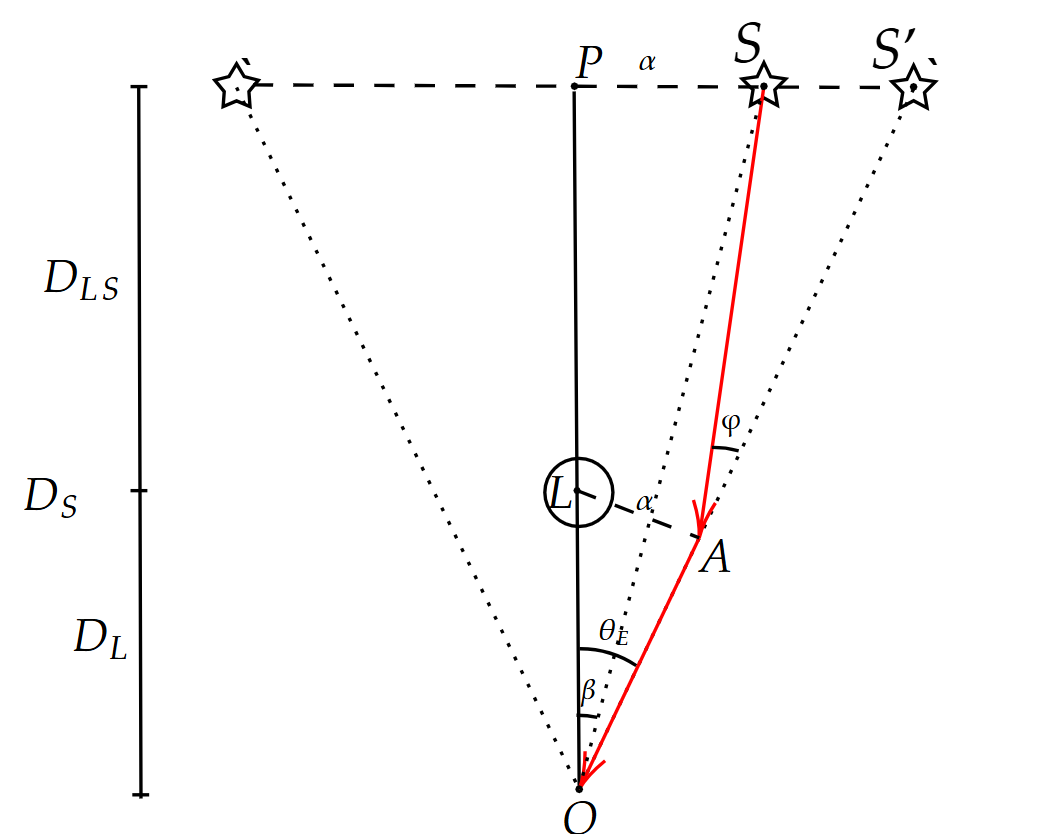
\includegraphics[width=0.9\linewidth]{imagens/anelE.png}
        \caption{Esquema da lente gravitacional}
    \end{figure}
    No esquema, o ponto \(O\) representa o observador, \(L\) o corpo massivo que atua como uma lente, \(S\) a posição real do objeto observado e \(S'\) sua posição aparente, \(\alpha\) é o parâmetro de impacto, \(\beta\) a separação angular entre o corpo observado e a lente, \(\theta_E\) o raio angular do anel de Einstein, \(\varphi\) o desvio angular causado por um corpo massivo. A distância \(\overline{OL}\) vale \(D_L\) e a distância \(\overline{OP}\) vale \(D_S\), de modo que \(D_S-D_L = D_{LS}\).

    Todos os ângulos são muito pequenos, de modo que \(\sin x \approx \tan x \approx x\). Além disso, por estarem no infinito, as retas \(\overline{OP}\), \(\overline{OS}\) e \(\overline{OS'}\) podem ser aproximadas como paralelas.

    É um resultado conhecido da Teoria da Relatividade Geral que o desvio da luz causado por um corpo massivo é dado por:
    \[\varphi = \frac{4GM}{\alpha c^2}\]
    \begin{alternativas}
        \item No limite em que \(\lim_{\alpha \rightarrow 0}\), encontre uma expressão para \(\theta_E\) em função das demais distâncias e ângulos fornecidos.
    
        \item O telescópio JWST obtém imagens no infravermelho, de comprimento de onda \(\lambda_{IV}\). Quão grande deve ser seu diâmetro para que ele possa resolver um anel de Einstein?
    \end{alternativas}

    \begin{pssolution*}{}{}
        \begin{alternativas}
            \item Note que, quando \(\alpha \rightarrow 0\), \(\overline{PL}=\overline{AS}=D_{LS}\). Utilizando \(\tan\theta = \sin\theta=\theta\), temos:
            
            \[(1)\ \overline{PS} = D_S\beta = \alpha, \ \ (2)\ \overline{SS'} = D_{SL}\varphi, \ \ (3)\ \overline{PS'} = D_S\theta_E,\] 
            \[(4)\ \overline{OL} = D_L = \overline{LA}/\theta_E = \alpha\theta_E, \ \ (5)\ \overline{LA}=\overline{PS}, \ \ (6)\ \overline{PS'} = \overline{PS}+\overline{SS'}\]

            Substituindo \((1), \ (2), \ (3)\) em \((6)\), 

            \[D_S\theta_E=D_S\beta+(D_S-D_L)\varphi\]

            \[\theta_E-\beta = \frac{D_S-D_L}{D_S}\varphi\]

            Substituindo o valor de \(\varphi\):

            \[\theta_E-\beta = \frac{D_S-D_L}{D_S}\frac{4GM}{\alpha c^2}\]

            Utilizando \((4)\), temos \(\alpha=D_L\theta_E\) e substituindo na nossa equação:

            \[\theta_E-\beta = \frac{D_S-D_L}{D_S}\frac{4GM}{D_L\theta_E c^2}\]

            \[\theta_E^2-\beta\theta_E = \frac{D_S-D_L}{D_S}\frac{4GM}{c^2}\]

            O limite de \(\alpha\rightarrow 0\) implica que \(\beta\rightarrow 0\), assim:

            \[\boxed{\theta_E=\sqrt{\frac{D_S-D_L}{D_S}\frac{4GM}{c^2}}}\]

            \item Utilizando o critério de Rayleigh \(\theta = R\frac{\lambda}{D}\), onde \(R\approx 1,22\). Isolando \(D\) e substituindo \(\theta = \theta_E\):
            
            \[\boxed{D =\sqrt{\frac{c^2R^2\lambda_{IV}^2}{4GM}\frac{D_S}{D_S-D_L}}}\]
        \end{alternativas}
    \end{pssolution*}
\end{pproblem}

\pts{4}
\begin{pproblem}
    Neste exercício, vamos estudar propriedades da excentricidade das órbitas e entender como ela se relaciona com a energia e o momento angular. Denotando \(\mu = GM\) e \(h=L/m\), faça o que se pede nos itens a seguir.
    \begin{center}
        \textbf{Parte I: O vetor excentricidade}
    \end{center}
    \begin{alternativas}
        \item Escreva uma expressão para a segunda lei de Newton no formato vetorial para um corpo de massa \(m\) orbitando um corpo de massa \(M\) a uma distância \(r\).
        
        \item Faça o produto vetorial da sua expressão por \(\mathbf{h}\) e prove que:
        
        \[\frac{d}{dt}(\dot{\mathbf{r}}\times \mathbf{h}) = \frac{\mu}{r}\mathbf{v} - \frac{\mu \dot{r}}{r^2}\mathbf{r}\]

        Onde \(\dot{\mathbf{r}}\) representa a velocidade radial e \(\mathbf{v}\) a velocidade.

        \item Podemos escrever o lado direito da equação anterior como:
        \[\frac{d}{dt}\left(A\mathbf{r}\right)\]

        Encontre o valor de \(A\).

        \item Integre os dois lados da igualdade encontrada e faça a multiplicação escalar de ambos os lados por \(\mathbf{r}\). Após isso, resolva para \(r\). O seu resultado deve ser bem parecido com o previsto somente pela geometria:
        \[r = \frac{p}{1+e\cos\theta}\]

        Encontre os valores de \(p\) e \(e\). \textbf{Não esqueça da constante de integração. Suas respostas podem depender dela.}

        \item No item anterior, \(e\) é a excentricidade da órbita. Voltando à equação obtida inicialmente no item \(c\), após a integração, ache uma forma de expressar \(\mathbf{e}\), como sendo um vetor de módulo \(e\) e que aponta diretamente para o corpo orbitado.
        
        \item Prove que a relação encontrada no item anterior pode ser escrita como:
        \[\mu \mathbf{e} = (v^2-\frac{\mu}{r})\mathbf{r} - (\mathbf{r}\cdot\mathbf{v})\mathbf{v}\]

        Para onde esse vetor aponta?
    \end{alternativas}
    \begin{center}
        \textbf{Parte II: Determinando elementos orbitais a partir do vetor excentricidade}     
    \end{center}
    Vamos definir o nosso sistema de coordenadas da seguinte maneira. Considere um sistema de mão direita, orientado de tal forma que o plano \(xy\) coincida com o plano equatorial e com \(\mathbf{z}\) apontando para o polo norte. Definindo o vetor nodal como \(\mathbf{n} = \mathbf{z} \times \mathbf{h}\).
    \begin{alternativas}
        \item Encontre uma expressão para \(\mathbf{h}\) em função das componentes do vetor \(\mathbf{r}\) e do vetor \(\mathbf{v}\). Após isso, encontre o vetor \(\mathbf{n}\) em função das componentes de \(\mathbf{h}\).

        \item Desenhe uma esfera celeste e represente nela: o plano do equador e uma órbita qualquer (que tenha inclinação diferente de 0). Nela, marque os seguintes ângulos: \(i\), a inclinação orbital, \(\Omega\) a longitude do nodo ascendente, \(\omega\) o argumento do periastro e \(\theta\), a anomalia verdadeira. 

        \item Encontre expressões para todos esses ângulos em função de \(\mathbf{e}\), \(\mathbf{h}\), \(\mathbf{n}\), \(\mathbf{r}\) e qualquer um dos vetores definidos no nosso sistema de coordenadas \(xyz\).
    \end{alternativas}

    \begin{pssolution*}{}{}
        \begin{center}
            \textbf{Parte I}
        \end{center}
        \begin{alternativas}
            \item Utilizando a forma vetorial da força gravitacional, temos:
            \[-\frac{GMm}{r^3}\mathbf{r} = m\ddot{\mathbf{r}} \rightarrow \boxed{\ddot{\mathbf{r}}= -\frac{\mu}{r^3}\mathbf{r}}\]

            \item Fazendo o produto vetorial dessa expressão por \(\mathbf{h}\), temos:
            
            \[\ddot{\mathbf{r}}\times \mathbf{h} = -\frac{\mu}{r^3}(\mathbf{r}\times\mathbf{h}) = \frac{\mu}{r^3}(\mathbf{h}\times\mathbf{r})\]

            Uma vez que \(\mathbf{h}\) é constante, o lado esquerdo da equação pode ser escrito como \(d(\dot{\mathbf{r}}\times \mathbf{h})/dt\). Para o lado direito, vamos escrever \(\mathbf{h} = \mathbf{r}\times \mathbf{v}\) e utilizar a regra do BAC-CAB, que diz que \((A \times B) \times C = B(A\cdot C) - C(A \cdot B)\). Desse modo:

            \[\frac{d}{dt}(\dot{\mathbf{r}}\times \mathbf{h}) = \frac{\mu}{r^3}((\mathbf{r}\times\mathbf{v})\times \mathbf{r}) = \frac{\mu}{r^3}(r^2\mathbf{v} - \mathbf{r}(\mathbf{r}\cdot \mathbf{v}))\]

            Note que \(\mathbf{r}\cdot\mathbf{v}\) é a multiplicação das componentes de \(\mathbf{r}\) e \(\mathbf{v}\) que estão na mesma direção. Assim, \(\mathbf{r}\cdot\mathbf{v} = r\dot{r}\). Substituindo na expressão anterior:

            \[\boxed{\frac{d}{dt}(\dot{\mathbf{r}}\times \mathbf{h}) = \frac{\mu}{r}\mathbf{v} - \frac{\mu \dot{r}}{r^2}\mathbf{r}}\]

            \item Abrindo a expressão fornecida pelo enunciado:
            
            \[\frac{d}{dt}(A\mathbf{r}) = \mathbf{r}\frac{d}{dt}A + A \mathbf{v}\]

            Comparando as expressões, é fácil perceber que \(\boxed{A = \mu/r}\).

            \item Utilizando as informações obtidas nos itens anteriores, temos:
            \[\frac{d}{dt}(\dot{\mathbf{r}}\times \mathbf{h}) = \mu\frac{d}{dt}\left(\frac{\mathbf{r}}{r}\right)\]

            Multiplicando ambos os lados por \(dt\) e integrando, temos:

            \[\dot{\mathbf{r}}\times\mathbf{h} = \frac{\mu}{r}\mathbf{r} + \mathbf{B}\]

            Onde \(B\) é um vetor constante de integração. Agora, fazendo o produto escalar com \(\mathbf{r}\):

            \[\mathbf{r}\cdot(\dot{\mathbf{r}}\times \mathbf{h}) = \mu r + \mathbf{r}\cdot\mathbf{B}\]

            Usando que \(a\cdot(b\times c) = (a\times b)\cdot c\) e definindo \(\nu\) como o ângulo entre \(\mathbf{r}\) e \(\mathbf{B}\), temos:

            \[h^2 = \mu r + rB\cos\nu\]

            Resolvendo para \(r\), chegamos em:

            \[r = \frac{h^2/\mu}{1+(B/\mu)\cos\nu}\]

            Assim:

            \[\boxed{p = \frac{h^2}{\mu}, \ \ \ \ e = \frac{B}{\mu}}\]

            \item Utilizando \(\mathbf{e} = \mu \mathbf{B}\) e voltando ao item \(d)\), temos:
            \[\dot{\mathbf{r}}\times \mathbf{h} = \frac{\mu}{r}\mathbf{r}+\mu \mathbf{e}\]

            Resolvendo para \(\mathbf{e}\) e notando que \(\dot{\mathbf{r}}\times\mathbf{h} = \mathbf{v}\times\mathbf{h}\), temos:

            \[\boxed{\mathbf{e} = \frac{\mathbf{v}\times\mathbf{h}}{\mu} - \frac{\mathbf{r}}{r}}\]

            \item Escrevendo \(\mathbf{h} = \mathbf{r}\times\mathbf{v}\), temos:
            \[\mathbf{e} = \frac{\mathbf{v}\times(\mathbf{r}\times\mathbf{v})}{\mu} - \frac{\mathbf{r}}{r} \]

            Multiplicando os dois lados da expressão por \(\mu\), e usando o BAC-CAB, temos:

            \[\mu\mathbf{e} = v^2\mathbf{r} - \mathbf{v}(\mathbf{v}\cdot\mathbf{r}) - \frac{\mu}{r}\mathbf{r}\]

            Reorganizando os termos:

            \[\boxed{\mu \mathbf{e} = (v^2-\frac{\mu}{r})\mathbf{r} - (\mathbf{r}\cdot\mathbf{v})\mathbf{v}}\]
        \end{alternativas}
    \end{pssolution*}
\end{pproblem}

\pts{5}
\begin{pproblem}\(\star\star\star\) (Adaptado IPhO 2018) Um dos efeitos mais interessantes da relatividade geral é a emissão de ondas gravitacionais (OG's) por binárias próximas. Um dos efeitos disso é a perda de energia do sistema. Nesta questão, iremos estudar esse efeito a fundo.

\begin{alternativas}
    \item Considere um sistema formado pelas estrelas 1 e 2, com massas \(M_i\) e distando \(r_i\) do centro de massa. Utilizando a segunda lei de Newton, é possível demonstrar que:
    \[\mathbf{a_1} = -\alpha \frac{\mathbf{r_1}}{r_1^n}\]
    Onde \(\mathbf{a_1}\) é o vetor aceleração da estrela 1. Encontre o valor de \(\alpha = \alpha (G, M_1, M_2)\) (lê-se \(\alpha\) em função de \(G, M_1, M_2\)) e de \(n\).

    \item A energia total do sistema binário pode ser expressa como:
    \[E = A(\omega, \mu, L) - \frac{GM\mu}{L}\]

    Onde \(\mu\) é a massa reduzida do sistema, \(M = M_1+M_2\) e \(L = r_1+r_2\). Encontre o valor de \(A\).

    \item A expressão anterior pode ser simplificada para:
    \[E = \frac{\beta GM\mu}{L}\]

    Onde \(\beta\) é uma constante adimensional. Encontre seu valor.

    A teoria correta da gravidade, a Relatividade Geral, foi formulada por Einstein em 1915 e prevê que a gravidade se propaga à velocidade da luz. Os mensageiros que carregam informações sobre a interação são chamados de ondas gravitacionais (OGs). OGs são emitidas sempre que massas são aceleradas, fazendo com que o sistema de massas perca energia.

    Considere um sistema de duas partículas pontuais, isoladas do restante do Universo. Einstein provou que, para velocidades suficientemente pequenas, as ondas emitidas: 1) têm uma frequência que é duas vezes maior do que a frequência orbital; 2) podem ser caracterizadas por uma luminosidade, ou seja, um poder emitido \(\mathcal{P}\), que é dominado pela fórmula:

    \[
    \mathcal{P} = \frac{G}{5c^5} \sum_{i=1}^3 \sum_{j=1}^3 \left( \frac{d^3 Q_{ij}}{dt^3} \right) \left( \frac{d^3 Q_{ij}}{dt^3} \right).
    \]

    Aqui, \( c \) é a velocidade da luz \( c \simeq 3 \times 10^8 \, \mathrm{m/s} \). Para um sistema de duas partículas pontuais orbitando no plano \( x-y \), \( Q_{ij} \) é a seguinte tabela (\( i, j \) indicam o número da linha/coluna):

    Os componentes de \( Q_{ij} \) são dados por:

    \[
    Q_{11} = \sum_{A=1}^2 \frac{M_A}{3} \left( 2x_A^2 - y_A^2 \right),
    \]

    \[
    Q_{22} = \sum_{A=1}^2 \frac{M_A}{3} \left( 2y_A^2 - x_A^2 \right),
    \]

    \[
    Q_{33} = -\sum_{A=1}^2 \frac{M_A}{3} \left( x_A^2 + y_A^2 \right),
    \]

    \[
    Q_{12} = Q_{21} = \sum_{A=1}^2 M_A x_A y_A.
    \]

    E \(Q_{i,j} = 0\) para todas as outras possibilidades. Aqui, \(x_A, y_A\) são as posições da estrela \(A\), com \(A=1,\ 2\) em um plano cartesiano com o centro de massa na origem.

    \item Escreva as coordenadas (\(x_1, y_1\)) e (\(x_2, y_2\)) em função de \(r_1, r_2, \omega\) e \(t\), com \(t\) sendo o tempo percorrido desde algum ponto específico da órbita.
    
    \item Para calcular a potência dissipada, a fórmula possui uma soma quádrupla. Resolver essa expressão "na tora" é algo bem complicado e demorado. Porém, felizmente, há um jeito mais bonito e elegante de resolvê-la. Para isso, comece escrevendo \(Q_{i,j}\) como uma matriz 3x3, da seguinte forma:
    
    \[Q = A\left(\begin{matrix}
        a_{11} & a_{12} & a_{13} \\
        a_{21} & a_{22} & a_{23} \\
        a_{31} & a_{23} & a_{33} \\
    \end{matrix}\right)\]

    Encontre o coeficiente \(A = A(\mu, L)\) e complete a matriz \(Q\).

    \item Do item anterior, você deve obter:
    \[Q_{ii} = A(b_i + j_i\cos(k t)), \ \ \ Q_{ij}^{i\neq j}= A(p_{ij} \sin(kt)) \]

    Encontre os valores de \(b_i\), \(j_i\), \(p_{ij}\) e \(k\).

    \item Agora, você é capaz de resolver para \(\mathcal{P}\) de maneira mais fluida. A expressão pode ser simplificada para:
    \[\mathcal{P} = \xi \frac{G}{c^5}\mu^2L^4\omega^6\]
    Encontre o valor numérico de \(\xi\).

    \textbf{DICA: } O somatório duplo:

    \[\sum_{i=1}^N\sum_{j=1}^N (A_{ij})(A_{ij})\]

    Onde \(A\) é uma matriz \(N\times N\) pode ser simplificado para:

    \[\sum_{i=1}^N\sum_{j=1}^N A_{ij}^2\]

    Que representa a soma quadrática de todos os elementos da matriz \(A\).

    \item Caso não houvesse a emissão de OG's, o sistema continuaria em equilíbrio indeterminadamente, mas devido à sua emissão, a energia do sistema não é conservada, fazendo com que haja uma variação na velocidade angular do sistema, \(\omega\). A fórmula para a variação temporal de \(\omega\) tem a seguinte cara:
    \[\left(\frac{d\omega}{dt}\right)^3 = (3\xi )^3 \frac{\omega^{11}}{c^{15}}(GM_C)^5\]
    
    Onde \(M_c\) é a chamada Massa \textit{Chirp} e \(M_c = M_c(M, \mu)\). Encontre uma fórmula para \(M_c\).

    \item Usando as informações obtidas acima, relacione a velocidade angular orbital \(\omega \) com a frequência das ondas gravitacionais \( f_{\text{OG}} \). Sabendo que, para qualquer função suave \( F(t) \) e \( a \neq 1 \):

    \[
    \frac{dF(t)}{dt} = \chi F(t)^a \implies F(t)^{1-a} = \chi (1-a)(t_0 - t),
    \]
    
    onde \( \chi \) é uma constante e \( t_0 \) é uma constante de integração, mostre que a equação do item anterior implica que a frequência das ondas gravitacionais é:
    
    \[
    f_{\text{OG}}^{-8/3} = 8\pi^{8/3} \xi \left( \frac{GM_c}{c^3} \right)^{(2/3)+p} (t_0 - t)^{2-p},
    \]
    
    e determine a constante \( p \).

    Em 14 de setembro de 2015, o evento GW150914 foi registrado pelos detectores LIGO, consistindo de dois braços em forma de L, cada um com 4 km de comprimento. Esses braços mudaram de comprimento relativo de acordo com a Figura abaixo. Os braços do detector respondem linearmente a uma onda gravitacional que passa, e o padrão de resposta imita a onda. Essa onda foi criada por dois buracos negros em órbitas quase circulares; a perda de energia por radiação gravitacional causou a contração da órbita e, eventualmente, a colisão dos buracos negros. O ponto de colisão corresponde, aproximadamente, ao pico do sinal após o ponto D, na Figura abaixo.

    \begin{figure}[H]
        \centering
        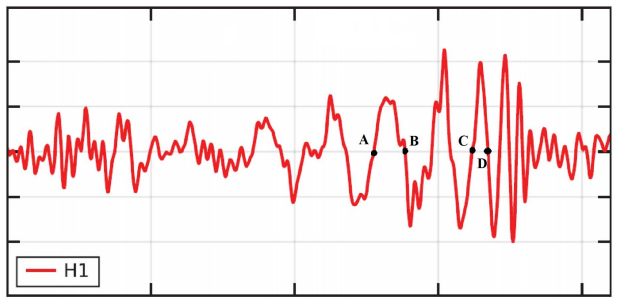
\includegraphics[width=0.7\linewidth]{imagens/grafico OG 1.png}
        \caption{Deformação, ou seja, variação relativa do tamanho de cada braço, no detector LIGO H1. O eixo horizontal representa o tempo, e os pontos A, B, C, D correspondem a \(t = 0,000\), \(0,009\), \(0,034\), \(0,040\) segundos, respectivamente.}
    \end{figure}

    \item A partir da figura, estime \( f_{OG}(t) \) em:

    \[
    t_{AB} = \frac{t_B + t_A}{2} \quad \text{e} \quad t_{CD} = \frac{t_D + t_C}{2}.
    \]
    
    Assumindo que a equação para \(f_{OG}\) é válida até a colisão (o que, estritamente falando, não é verdade) e que os dois objetos possuem massas iguais, estime a massa "chirp", \( M_c \), e a massa total do sistema, em termos de massas solares \( M_\odot \simeq 2 \times 10^{30} \, \text{kg}\).

    \item Estime a separação orbital mínima entre os dois objetos em \( t_{CD} \). 
    Assim, estime um tamanho máximo para cada objeto, \( R_{\text{max}} \). 
    Obtenha \( \frac{R_\odot}{R_{\text{max}}} \) para comparar esse tamanho com o raio do nosso Sol, \( R_\odot \simeq 7 \times 10^5 \, \text{km} \). 
    Estime também sua velocidade orbital linear no mesmo instante, \( v_{\text{col}} \), comparando-a com a velocidade da luz, \( \frac{v_{\text{col}}}{c} \).
\end{alternativas}

\begin{pssolution*}{}{}
    \begin{alternativas}
        \item Da segunda lei de newton, 
        \[-\frac{GM_1M_2}{(r_1+r_2)^3}\mathbf{d} = M_1\mathbf{a_1}\]

        Onde \(\mathbf{d}\) é um vetor que saí da estrela dois e vai até a estrela um. Portanto, \(|\mathbf{d}| = r_1+r_2\). Utilizando o teorema do centro de massa, temos 

        \[r_2 = \frac{M_1r_1}{M_2}\]

        Substituindo e simplificando, 

        \[\mathbf{a_1} = -\frac{GM_2}{r_1^3(1+\frac{M_1}{M_2})^3}\mathbf{d}\]

        Agora trabalhando no vetor \(\mathbf{d}\), note que a sua direção é a mesma direção que \(\mathbf{r_1}\), uma vez que a linha que liga 1 e 2, obrigatóriamente passa pelo CM do sistema. Assim, 

        \[\mathbf{d} = |\mathbf{d}|\hat{\mathbf{r_1}} = (r_1+r_2)\hat{\mathbf{r_1}} = (1+M_1/M_2)\mathbf{r_1}\]

        Substituindo, 

        \[\mathbf{a_1} = -\frac{GM_2}{(1+M_1/M_2)^2}\frac{\mathbf{r_1}}{r_1^3}\]

        Com isso, podemos concluir que 

        \[\boxed{\alpha = \frac{GM_2}{(1+M_1/M_2)^2}, \ \ \ n = 3 \ }\]

        \item A energia do sistema é dada por, 
        \[E = \frac{M_1v_1^2+M_2v_2^2}{2}-\frac{GM_1M_2}{L}\]

        Focando no primeiro termo e utilizando-se de que, \(v_A = r_A\omega\), temos 

        \[M_1v_1^2+M_2v_2^2 = (M_1r_1^2 + M_2r_2^2)\omega^2 \]

        Pelo teorema do centro de massa 

        \[(M_1r_1-M_2r_2)^2=0 \rightarrow M_1r_1^2 +M_2r^2_2 = \frac{M_1M_2}{M_1+M_2}L^2\equiv \mu L^2\]

        Para o segundo termo, basta multiplicar em cima e embaixo por \((M_1+M_2)\). Assim, 

        \[E = \frac{\mu L^2}{2} - \frac{G}{L}\frac{M_1M_2}{M_1+M_2}(M_1+M_2) \equiv \frac{\mu L^2\omega^2}{2} + \frac{GM\mu }{L}\]

        Desse modo, \(\boxed{A = \frac{\mu L^2\omega^2}{2}}\).

        \item Pela terceira lei de kepler, 
        
        \[\omega^2 = \frac{GM}{L^3}\]

        Substituindo, 

        \[E = \frac{GM\mu}{2L} - \frac{GM\mu}{L} = -\frac{GM\mu}{L}\]

        Concluindo assim, que \(\boxed{\beta = -1/2}\).

        \item Seja, \(\theta\) o ângulo que o vetor \(r_1\) faz com o eixo \(x\), desse modo, 
        \[(x_1, \ y_1) = r_1(\cos\theta, \ \sin\theta)\]

        O vetor \(r_2\) deve fazer um ângulo de \(\pi + \theta\). Utilizando que \(\sin(\pi+\theta) = -\sin(\theta)\) e \(\cos(\pi+\theta) = -\cos\theta\), 

        \[(x_2, \ y_2) = -r_2(\cos\theta, \sin\theta)\]

        Definindo por \(t\) o tempo decorrido desde que as estrelas cruzaram o eixo \(x\), tem se \(\theta = \omega t\). Logo, 

        \[\boxed{(x_1, \ y_1) = r_1 (\cos(\omega t), \ \sin(\omega t)) \ \ \ (x_2, \ y_2) = -r_2 (\cos(\omega t), \ \sin(\omega t))}\]

        \item A matrix terá a seguinte cara, 
        
        \[Q = \left(\begin{matrix}
            Q_{11} & Q_{12} & Q_{13} \\
            Q_{21} & Q_{22} & Q_{23} \\
            Q_{31} & Q_{32} & Q_{33} \\
        \end{matrix}\right)\]

        Evocando as fórmulas do enunciado, 
        \[
        Q_{11} = \sum_{A=1}^2 \frac{M_A}{3} \left( 2x_A^2 - y_A^2 \right),
        \]

        \[
        Q_{22} = \sum_{A=1}^2 \frac{M_A}{3} \left( 2y_A^2 - x_A^2 \right),
        \]

        \[
        Q_{33} = -\sum_{A=1}^2 \frac{M_A}{3} \left( x_A^2 + y_A^2 \right),
        \]

        \[
        Q_{12} = Q_{21} = \sum_{A=1}^2 M_A x_A y_A.
        \]

         Para \(Q_{11}\), temos, 

        \[Q_{11} = \frac{M_1}{3}(2x_1^2-y_1^2) + \frac{M_2}{3}(2x_2^2-y_2^2)\]

        Substituindo \(x\) e \(y\), 

        \[Q_{11} = \frac{M_1}{3}r_1^2(2\cos^2(\omega t) - \sin^2(\omega t)) + \frac{M_2r^2_2}{3}(2\cos^2(\omega t) - \sin^2(\omega t))\]

        \[Q_{11} = \frac{1}{3}(2\cos^2(\omega t) - \sin^2(\omega t))(M_1r_1^2 + M_2r_2^2)\]  
        \[Q_{11} = \frac{\mu L^2}{3}(2\cos^2(\omega t) - \sin^2(\omega t))\]

        Para \(Q_{22}\), 

        \[Q_{22} = \frac{M_1r_1^2}{3}(2\sin^2(\omega t) - \cos^2(\omega t)) + \frac{M_2r_2^2}{3}(2\sin^2(\omega t) - \cos^(\omega t))\]

        \[Q_{22} = \frac{\mu L^2}{3}(2\sin^2(\omega t) - \cos^2(\omega t))\]


        Para \(Q_{33}\)

        \[Q_{33} = -\frac{M_1r_1^2}{3}(\cos^2(\omega t) + \sin^2(\omega t))-\frac{M_2r_2^2}{3}(\cos^2(\omega t) + \sin^2(\omega t))\]

        \[Q_{33} = -\frac{\mu L^2}{3}\]

        Por fim, para \(Q_{12} = Q_{21}\), 

        \[Q_{12} = Q_{21} = M_1r_1^2\cos(\omega t) \sin(\omega t) + M_2r_2^2\cos(\omega t)\sin(\omega t)\]

        \[Q_{12} = Q_{21} = \mu L^2 \sin(\omega t)\cos(\omega t) = \frac{\mu L^2}{2}\sin(2\omega t)\]

        Como os de mais termos são \(0\), podemos escolher como \(A\) o valor de\(\mu L^2/2\), assim a nossa matriz \(Q\) toma forma, 

        \[Q = \frac{\mu L^2}{2}\left(\begin{matrix}
            \frac{4}{3}\cos^2(\omega t) - \frac{2}{3}\sin^2(\omega t)  & \sin(2\omega t) & 0 \\
            \sin(2\omega t) & \frac{4}{3}\sin^2(\omega t) - \frac{2}{3}\cos(\omega t) & 0 \\
            0 & 0 & -\frac{2}{3} \\
            \end{matrix}\right)\]

        Para os termos \(a_{11}\) e \(a_{22}\), vamos utilizar identidades trigonométricas, começando com \(a_{11}\), 
        \[\frac{4}{3}\cos^2(\omega t) - \frac{2}{3}\sin^2(\omega t) = \frac{2}{3}(2\cos^2(\omega t) - \sin^2(\omega t))\]

        Usando \(\cos^2(\omega t) = 1-\sin^2(\omega t)\), temos, 

        \[ = \frac{2}{3}\left(2-3\sin^{2}(\omega t)\right)\]

        Usando a forma do arco duplo, temos, 

        \[\cos(2x) = \cos^2x -\sin^2x = 1-2\sin^2x \rightarrow \sin^2x = \frac{1-\cos(2x)}{2}\]

        Fazendo essa substituição, 

        \[=\frac{2}{3}\left(2 - \frac{3}{2} + \frac{3}{2}\cos(2\omega t)\right) = \frac{1}{3}+\cos(2\omega t)\]

        Utilizando o mesmo processo para \(a_22\), encontramos
        \[a_{22} = \frac{1}{3}-\cos(2\omega t)\]

        De modo que nossa matriz pode ser simplificada para, 


        \[\boxed{Q = \left(\begin{matrix}
            \frac{1}{3}+\cos(2\omega t) & \sin(2\omega t) & 0 \\
            \sin(2\omega t) & \frac{1}{3} - \cos(2\omega t) & 0 \\
            0 & 0 & -\frac{2}{3} \\
        \end{matrix}\right)}\]

        \item Analisando a matriz anterior, temos que, 
        \[\boxed{A = \frac{\mu L^2}{2}}\]
        E que
        \[\boxed{b_1 = b_2 = \frac{1}{3}, \ \ b_3 = -\frac{2}{3}, \ \ j_1 = 1, \ \ j_2 = -1, \ \ j_3 = 0, \ \ p_{12}=p_{21} = 2, \ \ k= 2}\]

        \item A fórmula fornecida para a potência foi, 
        
        \[
        \mathcal{P} = \frac{G}{5c^5} \sum_{i=1}^3 \sum_{j=1}^3 \left( \frac{d^3 Q_{ij}}{dt^3} \right) \left( \frac{d^3 Q_{ij}}{dt^3} \right).
        \]

        Para começar, vamos derivar a matri \(Q\) com respeito ao tempo, 

        \[\frac{d^3 Q}{dt^3} = \frac{\mu L^2}{2}\frac{d^3}{dt^3}\left(\begin{matrix}
            \frac{1}{3}+\cos(2\omega t) & \sin(2\omega t) & 0 \\
            \sin(2\omega t) & \frac{1}{3} - \cos(2\omega t) & 0 \\
            0 & 0 & -\frac{2}{3} \\
        \end{matrix}\right)\]

        Para derivar uma matriz, basta derivarmos todos os seus elemtentos, ao fazer isso, chegamos em, 

        \[\frac{d^3Q}{dt^3} = \frac{\mu L^2}{2}\left(\begin{matrix}
            8\omega^3 \sin(2\omega t) & -8\omega ^3\cos(2\omega t) & 0 \\
            -8\omega^3\cos(\omega t) & -8\omega^3\sin(\omega t) & 0 \\
            0 & 0 & 0 \\ 
        \end{matrix}\right)\]

        Deixando o termo em como fora da matriz, 

        \[\frac{d^3Q}{dt^3} = 4\mu\omega^3L^2\left(\begin{matrix}
            \sin(2\omega t) & - \cos(2\omega t) & 0 \\
            -\cos(2\omega t) & - \sin(\omega t) & 0 \\
            0 & 0 & 0 \\
        \end{matrix}\right)\]

        Foi fornecido como dica que o termo 

        \[\sum_{i=1}^3 \sum_{j=1}^3 \left( \frac{d^3 Q_{ij}}{dt^3} \right) \left( \frac{d^3 Q_{ij}}{dt^3} \right)\]

        Corresponde a soma quadradica dos membros da matriz, desse modo 

        \[\sum_{i=1}^3 \sum_{j=1}^3 \left( \frac{d^3 Q_{ij}}{dt^3} \right) \left( \frac{d^3 Q_{ij}}{dt^3} \right) = (4\mu \omega^3 L^2)^2(\sin^2(2\omega t) + 2 \cos^2(\omega t))\]

        Assim, 

        \[\mathcal{P} = \frac{G}{5c^5} \sum_{i=1}^3 \sum_{j=1}^3 \left( \frac{d^3 Q_{ij}}{dt^3} \right) \left( \frac{d^3 Q_{ij}}{dt^3} \right) = \frac{G}{5c^5}(32\mu^2\omega^6 L^4)\]

        Reorganizando, 

        \[\mathcal{P} = \frac{32}{5}\frac{G\mu^2\omega^6L^4}{c^5}\]

        Comparando essa expressão com a fornecida pelo enunciado, temos, 

        \[\boxed{\xi = \frac{32}{5}}\]

        \item \(\mathcal{P}\) representa a potência que está sendo dissipada pelas OG's, assim, 
        \[\mathcal{P} = -\frac{dE}{dt}\]

        Igualando \(E\) a energia da órbita, 

        \[\mathcal{P} = \frac{GM\mu}{2} \frac{d}{dt}\frac{1}{L}\]

        Podemos escrever \(\omega\) em função de \(L\), para isso, basta utilizar a terceira lei de kepler, 


        \[\omega^2 = \frac{GM}{L^3} \rightarrow \frac{1}{L }= (GM)^{-1/3}\omega^{2/3}\]

        Substituindo, 

        \[\mathcal{P} = \frac{(GM)^{2/3}\mu}{2}\frac{d}{dt}\omega^{2/3} = \frac{(GM)^{2/3}\mu}{2}\frac{d}{d\omega}\omega^{2/3}\frac{d\omega}{dt}\]

        \[= \frac{(GM)^{2/3}\mu}{3\omega^{1/3}}\frac{d\omega}{dt}\]

        Igualando a expressão obtida no item anterior, 

        \[\frac{\xi G\mu^2\omega^6L^4}{c^5} = \frac{(GM)^{2/3}\mu}{3\omega^{1/3}}\frac{d\omega}{dt}\]

        Resolvendo para \(d\omega/dt\), 
        
        \[\frac{d\omega }{dt} = (3\xi)\frac{G\mu \omega^{19/3}L^4}{(GM)^{2/3}c^5}\]

        Substituindo \(L = \left(\frac{GM}{\omega^2}\right)^{1/3}\), temos, 

        \[\frac{d\omega}{dt} = (3\xi)\frac{G\mu \omega^{19/3}}{(GM)^{2/3}c^5}\left(\frac{GM}{\omega^2}\right)^{4/3}\]

        Elevando ao cubo, 

        \[\left(\frac{d\omega}{dt}\right)^{3} = (3\xi)^3\frac{G^3\mu^3\omega^{19}}{G^2M^2c^{15}}\frac{G^4M^4}{\omega^8}\]

        Simplificando, 

        \[\boxed{\left(\frac{d\omega}{dt}\right)^3 = (3\xi)^3\frac{\omega^{11}}{c^{{15}}}(G^5\mu^3M^2)}\]

        Analisabdo a expressão do enunciado, temos, 

        \[\boxed{M_c = (\mu^3 M^2)^{1/5}}\]

        \item Utilizando o fato fornecido pelo enunciado, 
        
        \[\frac{d F(t)}{dt} = \chi F(t)^a \rightarrow F(t)^{1-a} = \chi (1-a)(t_0-t)\]

        Podemos encontrar uma expressão para \(\omega(t)\).

        \[\frac{d\omega}{dt} = \frac{3\xi (GM_c)^{3/5}}{c^5}\omega^{11/3} \rightarrow \omega^{1-11/3} = \frac{3\xi (GM_c)^{3/5}}{c^5}(1-11/3)(t_0-t)\]

        Simplificando, 

        \[\omega ^{-8/3} = -\frac{3\xi (GM_c)^{3/5}}{c^5}\frac{8}{3}(t_0-t)\]

        \[\omega^{-8/3} = \frac{8\xi (GM_c)^{3/5}(t-t_0)}{c^5}\]

        Para encontrar uma expressão para \(f_{OG}\), temos que utilizar que, 

        \[f_{OG} = 2f_{orbt} = \frac{\omega}{\pi}\rightarrow \omega = \pi f_{OG}\]

        Fazendo tal substituição, chegamos em, 


        \[f_{OG}^{-8/3} = \frac{8\pi^{8/3}(GM_c)^{3/5}(t-t_0)}{c^5}\]

        Comparando com a forma do enunciado, podemos obter, 

        \[\boxed{p = 1}\]

        \item  A partir da figura, consideramos os dois $\Delta t$ como meias-períodos. Assim, a frequência de onda gravitacional cíclica é $f_{OG} = 1/(2 \Delta t)$. Então, os quatro pontos fornecidos nos permitem calcular a frequência no tempo médio dos dois intervalos como:

        \[
        \begin{array}{|c|c|}
        \hline
        t \, (\text{s}) & f_{OG} \, (\text{Hz}) \\
        \hline
        t_{AB} = 0.0045 & f_{OG}(t_{AB}) = (2 \times 0.009)^{-1} \\
        t_{CD} = 0.037 & f_{OG}(t_{CD}) = (2 \times 0.006)^{-1} \\
        \hline
        \end{array}
        \]
        
        Agora, temos dois pares de valores $(f_{OG}, t)$ para duas incógnitas $(t_0, M_c)$. Em termos de $t_{AB}$ e $t_{CD}$ e dividindo as duas equações, obtemos:
        
        \[
        t_0 = \frac{A t_{CD} - t_{AB}}{A - 1}, \quad A = \left( \frac{f_{OG}(t_{AB})}{f_{OG}(t_{CD})} \right)^{-8/3}.
        \]
        
        Substituindo os valores numéricos, $A \simeq 2.95$ e $t_0 \simeq 0.054 \, \text{s}$. Agora podemos usar a equação de \(f_{OG}\) para qualquer um dos valores $t_{AB}$ ou $t_{CD}$ e determinar $M_c$. Obtém-se a massa de chirp:
        
        \[
        M_c \simeq 6 \times 10^{31} \, \text{kg} \simeq 30 \, M_\odot\]
        
        Assim, a massa total $M$ é:
        
        \[
        M = 4^{3/5} M_c \simeq 69 \, M_\odot
        \]
        
        Este resultado é, na verdade, notavelmente próximo das melhores estimativas usando a teoria completa da Relatividade Geral! [Mesmo que os objetos reais não tenham massas exatamente iguais e a teoria que acabamos de usar não seja válida muito próximo da colisão.]
    
        \item Usando a lei de Kepler estabelece que $L = (GM / \Omega^2)^{1/3}$. O segundo par de pontos destacados no gráfico corresponde ao ciclo anterior à fusão. Assim, utilizando que \(f_{OG} = \omega/\pi\), 

        \[
        \omega_{t_{CD}} \sim 2.6 \times 10^2 \, \text{rad/s}.
        \]
        
        Em seguida, usando a massa total obtida anteriormente:
        
        \[
        L \sim 5 \times 10^2 \, \text{km}
        \]
        
        Assim, esses objetos possuem um raio máximo de $R_{\text{max}} \sim 250 \, \text{km}$. Portanto, eles têm mais de 30 vezes mais massa e:
        
        \[
        \frac{R_\odot}{R_{\text{max}}} \sim 3 \times 10^3,
        \]
        
        eles são 3000 vezes menores que o Sol!
        
        A velocidade linear é:
        
        \[
        v_{\text{col}} = \frac{L}{2} \omega \simeq 7 \times 10^4 \, \text{km/s}. 
        \]
        
        Eles estão se movendo a mais de 20\% da velocidade da luz!
        
        \[
        \boxed{
        \begin{aligned}
        \quad & L_{\text{col}} \sim 5 \times 10^2 \, \text{km}, \\
        & \frac{R_\odot}{R_{\text{max}}} \sim 3 \times 10^3, \\
        & \frac{v_{\text{col}}}{c} \sim 0.2.
        \end{aligned}
        }
        \]
    \end{alternativas}
    
\end{pssolution*}
\end{pproblem}

\pts{3}
\begin{pproblem}(Barra 2024) Durante sua estadia no Hotel Fazenda Ribeirão, Hugo observava a estrela Plo I com seu telescópio. Comparando o seu espectro com o de outras estrelas, ele descobre que Plo I é uma estrela de nêutrons e estima sua massa como sendo \( M_1 = 2M_{\odot} \). Ele também observa que Plo I possui variações senoidais em sua velocidade radial ao longo do tempo e conclui que Plo I deve fazer parte de um sistema binário com outro corpo celeste, Plo II. Observando a curva de velocidade de Plo I, Hugo também determina que Plo I possui uma órbita circular de período \( P \) e velocidade radial máxima \( K \). Porém, ele não sabe qual é a massa \( M_2 \) de Plo II e nem qual é a inclinação \( i \) do plano orbital do binário em relação ao plano do céu, representada na figura a seguir.

    \begin{figure}[H]
        \centering
        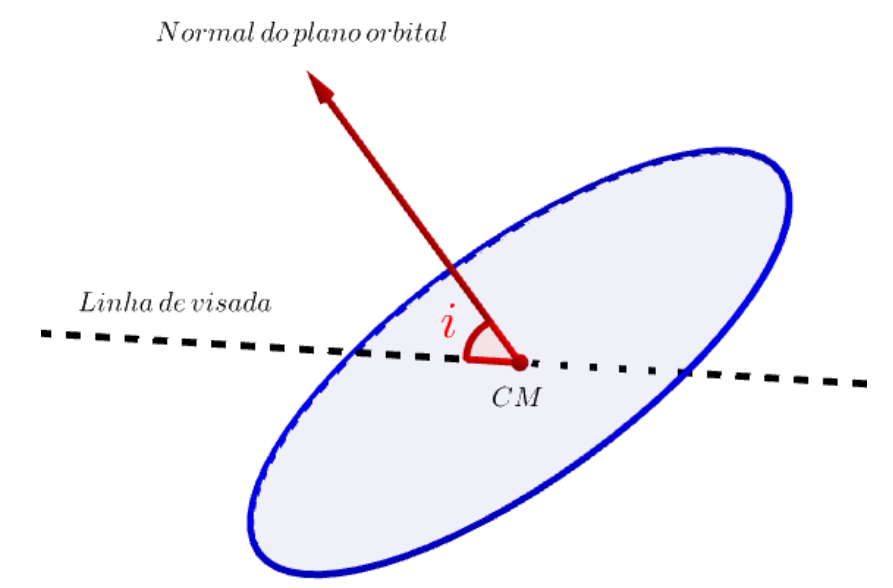
\includegraphics[width=0.8\linewidth]{imagens/figurabarra.png}
        \caption{Representação da órbita}
    \end{figure}

    \begin{alternativas}
        \item A partir da 3ª lei de Kepler e da 2ª lei de Newton, encontre uma expressão para a \textbf{função de massa} do sistema binário formado por Plo I e Plo II em termos de \( P \), \( K \) e constantes universais. Você pode utilizar que a função de massa é dada por:
        \[
            f = \frac{M_2^3 \sin^3 i}{(M_1 + M_2)^2}
        \]
    
        \item Utilizando suas medidas, Hugo calcula que a função de massa do binário é \( f = 46,2M_{\odot} \). Desejamos encontrar o valor mínimo \( M_{2,\text{min}} \) para a massa de Plo II, sabendo que ele corresponde ao caso em que \( i = 90^\circ \). Suponha \( M_{2,\text{min}} > M_1 \). A partir disso, determine \( M_{2,\text{min}} \). Seu resultado é condizente com a hipótese? Responda SIM ou NÃO, justificando com cálculos.
        
        \item Com base em sua resposta do item anterior, conclua: é mais provável que Plo II seja um exoplaneta, uma anã branca, uma estrela de nêutrons ou um buraco negro?
    \end{alternativas}
    \begin{pssolution*}{}{}
        \begin{alternativas}
            \item Primeiramente, note que \(v_{r, aparente} = |\mathbf{\omega}\times\mathbf{r}| = \omega r \sin i = v_r \sin i\), logo \(K = v_r\sin i = \frac{2\pi a_1}{T}\sin i\). Defindino \(a=a_1+a_2\) e \(M = M_1+M_2\) onde \(a_i\) e \(M_i\) representam a distância entre a estrela \(i\) e o CM e a massa da estrela \(i\), temos a terceira lei de kepler como, 
            \[\frac{a^3}{T^2} = \frac{GM}{4\pi^2}\]
        \end{alternativas}
    \end{pssolution*}
    
    
\end{pproblem}

\newpage

\section{Astronomia de Posição}

\pts{5} %problema da semana 114
    \begin{pproblem} Após se perderem em uma navegação, você e o professor Klafke, naufraga em uma ilha e encontra o seguinte relógio de Sol:
        \begin{figure}[H]
            \centering
            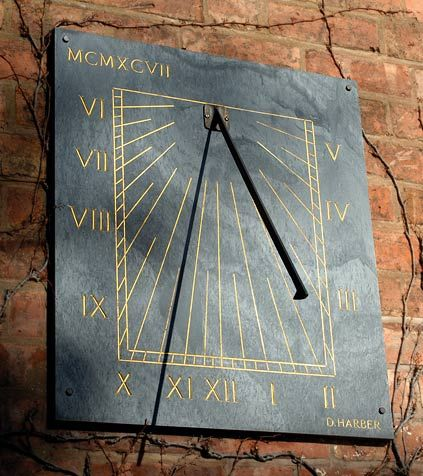
\includegraphics[width=0.5\linewidth]{imagens/q6.jpg}
            \caption{Relógio de Sol}
        \end{figure}
        Agora é missão de vocês descobrirem propriedades do relógio de Sol.
        \begin{enumerate}[label=\textbf{\alph*)}]
            \item Em qual hemisfério vocês se encontraram? Como você chegou a tal conclusão?
            \item Após várias semanas na ilha, vocês notam que a sombra do relógio parece seguir uma linha reta, sendo \(\phi\) a latitude que vocês se encontraram, determine a declinação do Sol nesse dia e explique o porquê disso só acontecer em \(2\) dias do ano.
            \item Prove que, quando o Sol possuí a declinação encontrada anteriormente, a sombra segue uma linha reta. Isso pode ser feito seguindo os seguintes passos:
            \begin{enumerate}[label=\roman*)]
                \item Determine a orientação da linha e explicar por que ela deve estar nessa orientação;
                \item Determine o comprimento da sombra para uma dada posição do Sol em coordenadas alt-azimute;
                \item Derivar uma relação entre altitude e azimute, dado que a ponta da sombra está sobre a linha;
                \item Determine uma quantidade constante e mostrar que ela é constante para todas as posições do Sol naquele dia.
            \end{enumerate}
        \end{enumerate}
    
    
    \begin{pssolution*}{}{}
        \begin{alternativas}
            \item Pela imagem, podemos notar que as notações da esquerda correspondem as horas da manhã. Assim, temos que o Sol está nascedo á direita, para que assim a sua sombra fique sobre a esquerda. A partir desses argumentos, é possivel dizer que o ponto cardeal \textit{Leste} se encontra a direita e o \textit{Oeste} a direita. Um relógio de sol vertical, tem seu gnômon sempre apontado para o polo celeste não elevado. Como este está apontando para a direção \textit{Sul}, podemos concluir que o relógio se encontra no \(\boxed{\textit{hemisfério Norte}}\).
          
            \item Isso só acontece nos equinócios, quando \(\delta_\odot = 0\).
            
            \item Seguindo os passos do enunciado, 
            \begin{enumerate}[label=\roman*)]
                \item Como \(\delta_\odot=0\), o céu se move exatamente da direção leste para oeste, 
                \item Se o gnônom tem comprimento \(L\) e o Sol está em uma altura \(h\), utilizando geometria, podemos dizer que o comprimento da sombra, \(l\) vale, \(l=\frac{L}{\tan h}\).
                \item Observe a seguinte figura, 
                \begin{figure}[H]
                    \centering
                    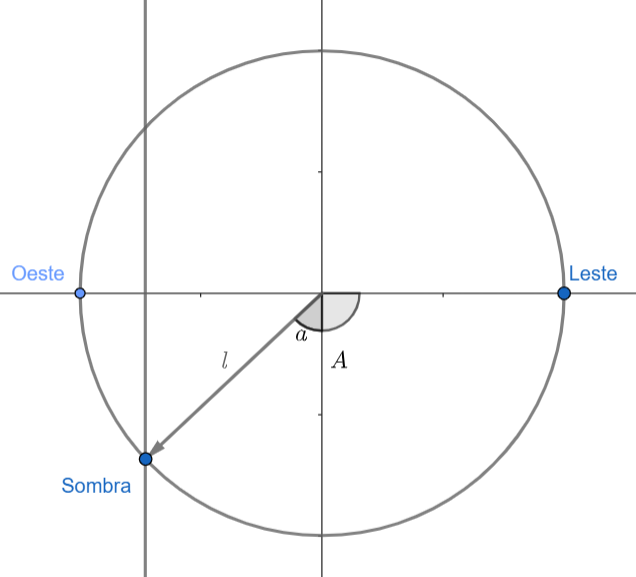
\includegraphics[width=0.66\linewidth]{imagens/retarelogiosolvert.png}
                    \caption{Esquema da linha imaginaria}
                \end{figure}
            \end{enumerate}
            
            A distância entre o centro do reógio e a sombra é dada por,

            \[x = l\sin (A-90^{\circ})\equiv l\sin a = L\frac{\sin a}{\tan h}\]

            Agora, queremos provar que essa quantidade é constante.

            \item Observe o seguinte triângulo, 
            
            \begin{figure}[H]
                \centering
                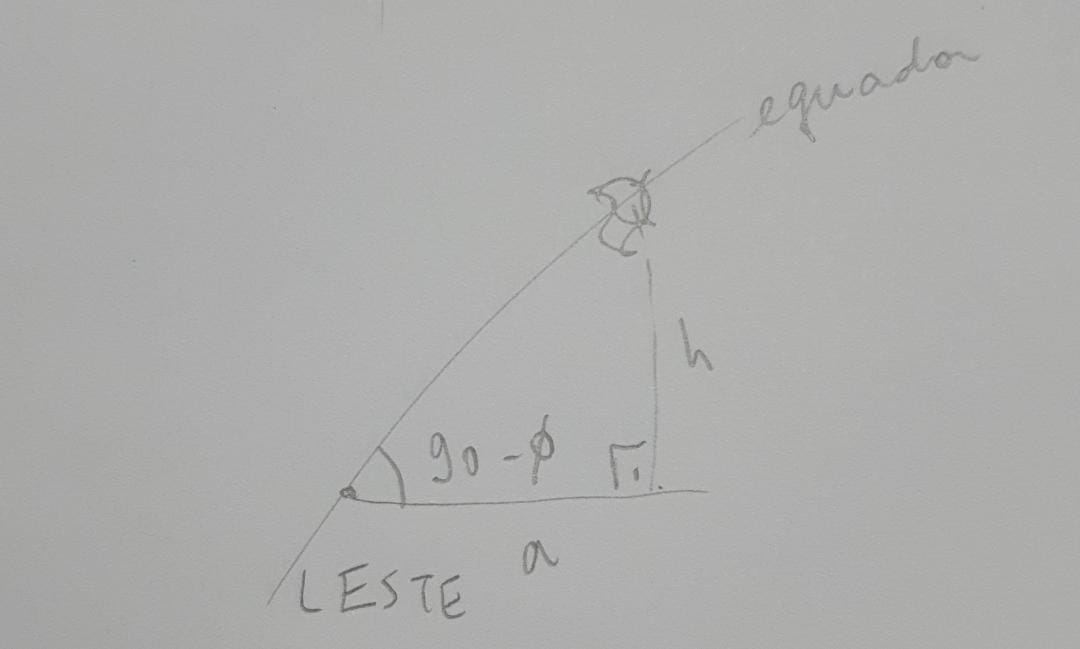
\includegraphics[width=0.5\linewidth]{imagens/trigesf1.jpg}
                \caption{Sol no equador}
            \end{figure}

            Usando a Lei dos quatro elementos, 

            \[\cot(90^\circ -\phi)\sin(90^{\circ})+\cos a \cos(90) = \cot h \sin a\]

            Simplificando, temos, 

            \[\frac{\sin a}{\tan h } = \tan {\phi}\]

            O que é constante. Logo, a nossa condição está provada.
            

        \end{alternativas}
    \end{pssolution*}
    \end{pproblem}

    \pts{5}
    \begin{pproblem} (Adaptado T1 - 2024)
        A equação do tempo é a diferença entre a ascenção reta do Sol médio e a ascenção reta do Sol verdadeiro. Sabendo disso, vamos calcular algumas das suas propriedades.
        \begin{alternativas}
            \item Determine uma expressão para a equação do tempo, desconsiderando a excentricidade da Terra, i.e.: O Sol possuíndo velocidade constante ao longo da ecliptica. Deixe sua resposta em função do tempo desde o equinócio de março \(T_M\), do período da Terra \(T\) e da obliquidade da eclíptica \(\epsilon\).
            \item Agora, considerando a excentricidade da Terra, a equação do tempo tem forma:
            \[E.T. = -2e \cdot \sin(k_1 \cdot M) + \tan^2 \left( \frac{\epsilon}{2} \right) \cdot \sin\left( k_2 \cdot (M + \lambda_P) \right)\]
            Onde \(M\) é a anomalia média, \(\lambda_P\) a longitude eclíptica do periastro e \(e\) a excentricidade da Terra. Determine as constantes \(k_1\) e \(k_2\). Pense nas situações de simetria envolvendo cada uma das parcelas da equação.
            \\
            Agora o objetivo da questão é descobrir a declinação do Sol no ponto de nó do analema. Veja a figura a seguir:
            \begin{figure}[H]
                \centering
                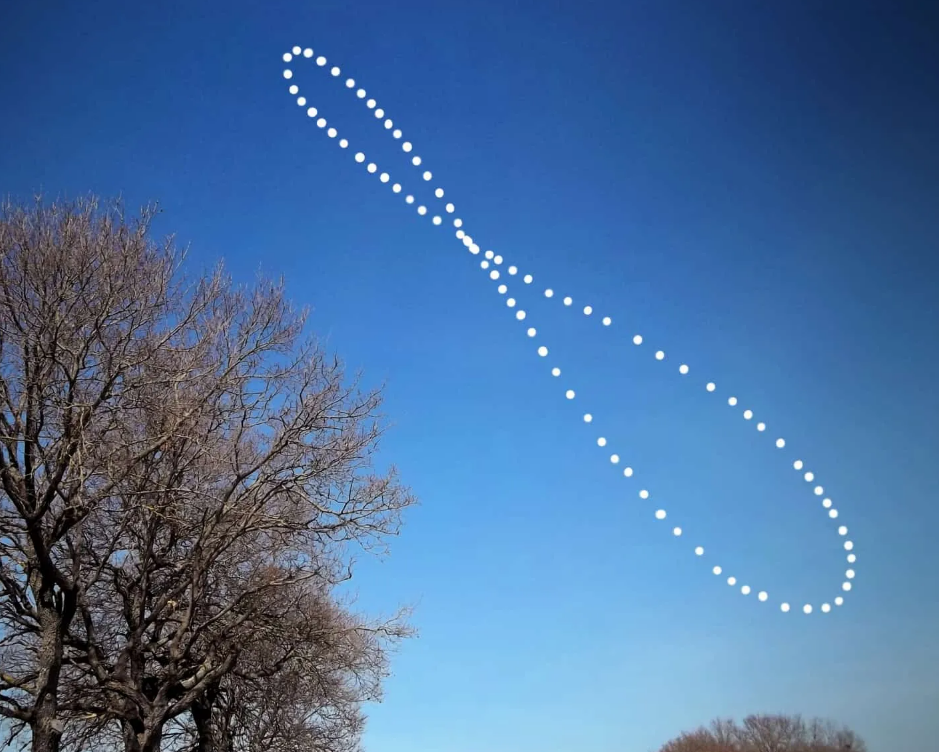
\includegraphics[width=0.7\textwidth]{imagens/q16.png}
                \caption{Representação analema}
            \end{figure}
            O ponto de nó é o ponto em que a trajetória se cruza.
            \item Para pequenos valores da declinaçãop do Sol, obtenha uma fórmula para essa em função de \(M\), \(\lambda_P\) e \(\epsilon\). Considere também que a excentricidade e a inclinação da órbita sejam suficientemente pequanos pequenos.
            \item Encontre as duas anomalias médias que tenham a mesma declinação e mesma \(E.T.\).
            \item Encontre o valor da declinação Solar no ponto de nó.
        \end{alternativas}
    
    \begin{pssolution*}{}{}
        \begin{alternativas}
            \item A equação do tempo se da por
            
            \[E.T. = \alpha_M - \alpha_V\]

            Onde \(\alpha_M\) é a ascenção reta do Sol médio, i.e.: um "Sol fictício" que se move ao longo do equador com velocidade constante, e \(\alpha_V\) a ascenção reta do Sol verdadeiro.

            Observe o seguinte triângilo esférico

            COLOCAR imagem

            Primeiramente, tanto o Sol verdadeiro quando o Sol médio possuem velocidades angulares constantes e equivalentes a \(\omega_\odot = 2\pi/T\), assim, \(\alpha_M=\omega_\odot T_M\).

            Utilizando a lei dos quatro elementos

            \[\cot \pi/2 \sin\epsilon + \cos\epsilon\cos\alpha_V=\cot(\omega_\odot T_M)\sin\alpha_V\]

            Como \(\cot\pi/2 =0\), obtemos

            \[\alpha_V = \tan^{-1}(\cos\epsilon\tan(\omega_\odot T_M))\]

            Note que, quando \(\epsilon = 0\), \(\alpha_V = \alpha_M\) como esperado.

            Por fim, voltando a definição da equação do tmepo

            \[\boxed{E.T. = \tan^{-1}\left(\cos\epsilon\tan\left(\frac{2\pi}{T} T_M\right)\right) - \frac{2\pi}{T}T_M}\]

            \item Para resolver essa questão, vamos pensar nas situações de simetria. Para uma órbita Elipstica, a unica situação de simetria é em relação ao eixo maior. Já considerando a obliquidade da eclíptica, existem duas simetrias possiveis, em relação a linha dos soltiscios e dos equiócios. Por tanto é razoavel pensar que a senoide que se relaciona com a excentricidade da órbita tenha um período por ano enquanto a que se relaciona com a obliquidade da eclptica tenha 2 perídos por ano, assim \(\boxed{k_1=1, \ k_2 = 2}\)
            
            \item Voltando ao triângulos esférico anterior e utilizando a Lei dos Senos, nós temos
            
            \[\frac{\sin\delta_\odot}{\sin\epsilon} = \sin\lambda\]

            Onde \(\lambda \) é a longitude ecliptica do Sol. Utilizando que para pequanos ângulos \(\sin\theta \approx \theta\), temos

            \[\delta_\odot = \epsilon\sin\lambda\]

            Desprezando a excentricidade, temos \(\lambda = \lambda_P + M\), assim

            \[\boxed{\delta_\odot = \epsilon\sin(\lambda_P + M)}\]

            \item A condição para que duas anomalias médias possuam a mesma equação do tempo é 
            \[\sin(M_1+\lambda_P) = \sin(M_2+\lambda_P)\]

            Usando que \(\sin\theta = \sin(\pi-\theta)\) temos

            \[\boxed{M_2 =\pi -M_1-2\lambda_P}\]

            \item Igualando as equações do tempo
            
            \[-2e\sin(M_1) + \tan^2 \left( \frac{\epsilon}{2} \right)\sin\left(2(M_1 + \lambda_P) \right) = -2e\sin(M_2) + \tan^2 \left( \frac{\epsilon}{2} \right)\sin\left(2(M_2 + \lambda_P) \right)\]

            Substituindo \(M_2\)  

            \[-2e\sin(M_1) + \tan^2 \left( \frac{\epsilon}{2} \right)\sin\left(2(M_1 + \lambda_P) \right) = -2e\sin(M_1+2\lambda_P) - \tan^2 \left( \frac{\epsilon}{2} \right)\sin\left(2M_1 + 2\lambda_P \right)\]

            \[\tan^2 \left( \frac{\epsilon}{2} \right)\sin(2M_1+2\lambda_P) = e(\sin M_1 - \sin(M_1+\lambda_P))\]

            Utilizando o seno do arco duplo e prostaférese:

            \[\tan^2\left(\frac{\epsilon}{2}\right)\sin(M_1+\lambda_P)\cos(M_1+\lambda_P) = -e\sin\lambda_P\cos(M_1+\lambda_P)\]

            \[\sin(M_1+\lambda_P) = -\frac{e\sin\lambda_P}{\tan^2\left(\frac{\epsilon}{2}\right)}\approx -\frac{4e\sin\lambda_P}{\epsilon^2}\]

            Finalmente, substituindo na fórmula da declinação:

            \[\boxed{\delta_\odot \approx -\frac{4e\sin\lambda_P}{\epsilon}}\]
        \end{alternativas}
    \end{pssolution*}
    \end{pproblem}

    
\pts{5}
\begin{pproblem}
    Porílio, após um longo dia de aulas no ITA, no solstício de verão (\(\phi =23^\circ 11' S, \ \lambda= 45^\circ53' O\)). No dia em questão, o valor da equação do tempo é \(E.T. = -3\) minutos. Porílio, não quer perder o Sol de jeito nenhum e começa a correr para que o (centro do) Sol continue no horizonte.

    \begin{alternativas}
        \item São José dos Campos, segue o horário de Brasília (UTC-3h), em qual horário, no Tempo Civil, Porílio deve começar sua corrida?
        \item Se Porílio corre em direção a um dos polos geográficos, qual deve ser a sua velocidade inicial?
        \item Se Porílio decide subir uma montanha de inclinação \(i = 30^\circ\), a uma velocidade constante de \(v = 1\) m/s, qual o maior tempo com que Porílio consegue deixar o Sol acima do horizonte?
        \textbf{Dica: } Utilizar aproxiamações para pequenos angulos, talvez seja util
    \end{alternativas}

\begin{pssolution*}{}{}
    \begin{alternativas}
        \item Para encontrar o horário de nascer/se por de uma estrela, precisamos achar o ângulo horário dela no momento em que ela nasce. Olhe o triângulo esférico a seguir, 
        
        \begin{figure}[H]
            \centering
            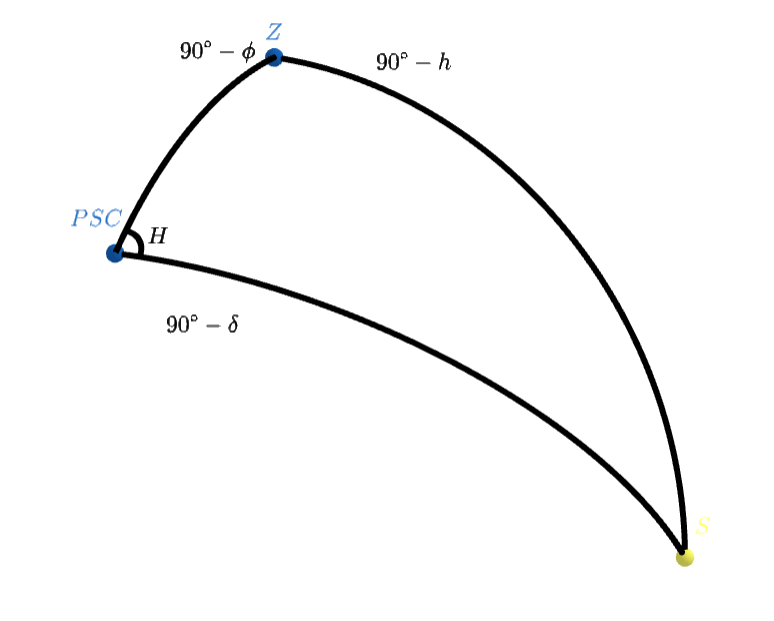
\includegraphics[width=0.8\linewidth]{imagens/trigangulohorario.png}
            \caption{Esquema do Sol no Horizonte}
        \end{figure}

        No momento em que o sol se encontra no horizonte, temos \(h=0\). Por ser solstício de verão (no hemisfério Sul), temos \(\delta = -23,47^\circ\). Utilizando uma lei dos cossenos e que \(\sin(90-\theta) = \cos(\theta)\) e que \(\cos(90-\theta) = \sin(\theta)\), temos 

        \[\sin h = \sin\phi\sin\delta +\cos\phi\cos\delta\cos H\]

        Resolvendo para \(H\), e usando \(\sin h = \sin 0^\circ = 0\), 

        \[\cos H = -\tan\phi\tan\delta\]

        Resolvendo, obtemos \(H = 100,72^\circ = 6^h42^m52^s\)

        O horário do por do Sol, é dado por \(TSL = 12+H = 18^h42^m52^s\).

        Utilizando que \(TC = TSL + (\lambda_{fuso}-\lambda_{local})/15 - E.T.\), obtemos, 

        \[\boxed{TC = 18^h49^m20^s}\]

        \item Porílio deve correr em direção ao Polo Celeste Sul, uma vez que ele a declianção do Sol é negativa. Para achar sua velocidade inicial, vamos derivar a lei dos cossenos em relação ao tempo em \(h=0\).
        \[\frac{d\cos H}{dt} = -\tan\delta \frac{d\tan\phi}{dt}\]

        Usando a regra da cadeia, 

        \[-\sin H \dot{H} = -\frac{\tan\delta}{\cos^2\phi}\dot{\phi}\]

        Onte \(\dot{a} = \frac{da}{dt}\). Isoloando \(\dot{\phi}\), 

        \[\dot{\phi} = \frac{\cos^2\phi\sin H}{\tan\delta}\dot{H}\]

        A variação do ângulo horario é \(360^\circ/24^h = 15^\circ/1^h\). Resolvendo para \(\dot{\phi}\), 

        \[\dot{\phi} = \frac{-28,68^\circ}{h} = -1,39\cdot 10^{-4}\text{ rad/s}\]

        Note que o sinal de \(\dot{\phi}\) apenas representa que ele está se movendo em direção ao polo Sul. Utilizando que, 

        \[\dot{\phi} = \frac{v}{R_\oplus}\]

        Chegamos na relação \(v = R_\oplus|\dot{\phi}|\),
        
        \[\boxed{v \approx 885 \text{ m/s}}\]

        \item Agora, temos que usar a ideia de ângulo do horizonte. Observe a seguinte imagem, 
            \begin{figure}[H]
                \centering
                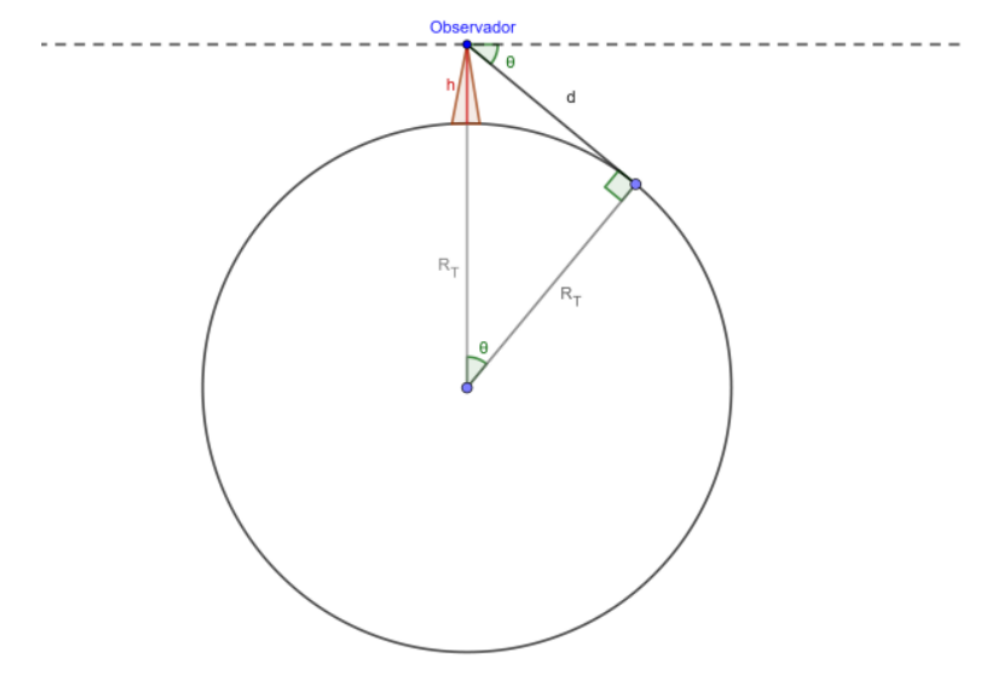
\includegraphics[width=0.90\linewidth]{imagens/angulohorizonte.png}
                \caption{Fonte: Apostila Magna}
            \end{figure}

            O ângulo \(\theta\), vale

            \[\cos\theta = \frac{R_T}{R_T+h}\]

            Como \(h<<R_T\), vamos utilizar \(x=h/R_T\) e usar a aproxiamações para \(x<<1\).

            \[\cos\theta = \left(\frac{R_T+h}{R_t}\right)^{-1} = \left(1+\frac{h}{R_T}\right)^{-1} \approx 1-\frac{h}{R_T}\]

            Como \(\theta\) é um ângulo pequeno, vamos utilizar a aproximação em segunda ordem utilizando a série de taylor, 

            \[f(x) \approx \sum\frac{f^{(n)}(a)x^n}{n!}\]

            Onde \(f^{(n)}(x)\) representa a n-ésima derivada de \(f(x)\). Espandindo a função em torno de \(a=0\), temos, 

            \[\cos\theta \approx 1 -\frac{\theta^2}{2}\]

            Igualando os termos, 

            \[1-\frac{\theta^2}{2} = 1-\frac{h}{R_T} \rightarrow \theta = \sqrt{\frac{2h}{R_T}}\]

            Para calcular o tempo em qeu o sol continua acima do horizonte, temos que calcular o tempo em que a altura aparente do sol, deve ser compensada pelo angulo \(\theta\), afim de que o sol permaneça no horizonde. Desse modo, a lei dos cossenos, se torna, 

            \[\sin\theta = \sin\phi\sin\delta + \cos\phi\cos\delta\cos H\]

            Usando \(\sin\theta\approx \theta\), 

            \[\theta = \sin\phi\sin\delta+\cos\phi\cos\delta \cos H\]

            Derivando dos dois lados com relaçcao ao tempo, (aqui vamos desprezar \(\dot{\phi}\) uma vez que a velocidade com que Porílio se move é muito pequena).

            \[\frac{d\theta}{dt} = -\cos\phi\cos\delta\sin H \dot{H}\]

            Para derivar \(\theta\) em relação ao tempo, perceba que \(h(t) = v t \sin i\).

            \[\frac{d\theta}{dt} = \sqrt{\frac{2v\sin i }{R_T}}\frac{d}{dt}\sqrt{t} = \sqrt{\frac{v\sin i}{2 R_T t}}\]

            Igualando as expressões, 

            \[\frac{v\sin i}{2R_T t} = (\cos\phi\cos\delta\sin H \dot{H})^2\]

            \[t = \frac{v\sin i}{2R_T(\cos\phi\cos\delta\sin H \dot{H})^2}\]

            \[\boxed{t \approx 10,82\text{ s}}\]

        \end{alternativas}
    
\end{pssolution*}
\end{pproblem}

    \pts{3}
    \begin{pproblem}
        Mauí, um renomado astrônomo deseja passar as suas férias de fim de ano em Serjipe \((10^\circ \ 54'\ 33'' S, \ 37^\circ 4'29'' O\)) e deseja saber o horario de nascimento de uma das suas estrelas favoritas, All Kaf al Dij Ma \Romannum{3} \((\delta = +10^\circ \ 56'\ 58'', \ \alpha = 2h \ 58m \ 43s\)) e precisa da sua ajuda para calcular o horário de nascimento dela nas seguitnes situações:
        \begin{alternativas}
            \item Calcule o horário de nascimento de All Kaf al Dij Ma \Romannum{3} no solstício de dezembro.
            \item Quando tempo a estrela passará acima do horizonte?
            \item Estime o período de tempo em que a estrela é visível.
        \end{alternativas}

    \begin{pssolution*}{}{}
        \begin{alternativas}
            \item Como visto anteriormente, o ângulo horário de nascer de uma estrela é calculadro por, 

        \[\cos H = - \tan \delta \tan \phi \rightarrow H = \]

        O horário pode ser obtido usando a equação, 

        \[TSL = \alpha + H\]

        Resultando em \(\boxed{TSL = }\)

        \item O tempo em que a estrela fica acima do horizonte é dado por, 
        
        \[\Delta t = 2 H = \]

        \item No solstício de verão, \(\delta_\odot = -23,47\), assim, o ângulo horário do sol é dado por, \(H_\odot = -\tan\delta_\odot \tan\phi = \), Ou seja, o tempo em que o Sol fica visível é dado por, \(\delta t_\odot = \). Uma estimativa valida do tempo em que a estrela é vísivel, é dada por, 
        \[\Delta t = 2 (H - H_\odot)\]

        Que representam os períodos em que a estrela esterá acima do horizonte sem a presença do Sol, 
       
        \[\boxed{\Delta t = }\]
    \end{alternativas}
        
        
    \end{pssolution*}
    \end{pproblem}

    \pts{4}
    \begin{pproblem}(Lucas Cavalcante - \href{https://noic.com.br/olimpiadas/astronomia/problemas-da-semana/astronomia-semana-111/}{Semana 111})
        Considerando um sistema de coordenadas horizontal em que o azimute \(0\) corresponde ao ponto cardeal norte, um asteroide foi observado nas alturas \(h_1\) e \(h_2\) e azimutes \(A_1\) e \(A_2\). enquanto outro asteroide foi observado nas coordenadas \(h_3\), \(h_4\), \(A_3\) e \(A_4\). Encontre as coordenadas dos pontos de encontro entre os asteroides.
        
        \begin{psidea}{Notação de Einsten}{}
        Durante a resolução dessa questão, utilizarei a Notação de Einsten. Ela é uma ferramente física para facilitar as contas vetoriais. Explicando, na notação comum, um vetor é representado por
        \[\mathbf{a} = (a_1 \hat{\mathbf{e}}_1, \ a_2 \hat{\mathbf{e}}_2, \ a_3 \hat{\mathbf{e}}_3)\]
        Na notação de Einsete, isso é substituido por:
        \[\mathbf{a} = a_i \hat{\mathbf{e}}_i\]
        Onde os indíces repedidos indicam a soma (\(a_i \hat{\mathbf{e}}_i = a_1 \hat{\mathbf{e}}_1+a_2 \hat{\mathbf{e}}_2+a_3 \hat{\mathbf{e}}_3+...\))
        
        O produto escalar entre dois verores, na notação de Einsten é definido por:

        \[\mathbf{a}\cdot \mathbf{b} = a_ib_j\delta{ij}\]

        Onde \(\delta_{ij}\) é a função \textit{Delta de Kronecher} e é definida por:

        \[\delta_{ij} = \left \{ \begin{matrix} 0, & \mbox{se } i \ne j \\ 
                                                1, & \mbox{se } i = j\end{matrix} \right.\]
            
        Assim, \(\mathbf{a}\cdot \mathbf{b} = a_ib_i \equiv a_1b_1 +a_2b_2 + a_3b_3\)

        Já para o produto vetorial, temos:
            \[
            \mathbf{a} \times \mathbf{b} = a_i b_j \Epsilon_{ijk} \hat{\mathbf{e}}_k
            \]
            Aqui, \(\Epsilon_{ijk}\) é denominado \textit{tensor de Levi-Civita}, ou símbolo de Levi-Civita, e é definido como:

            \[
            \Epsilon_{ijk} = 
            \begin{cases} 
            +1 & \text{se } (i, j, k) \text{ é uma permutação par de } (1, 2, 3), \\
            -1 & \text{se } (i, j, k) \text{ é uma permutação ímpar de } (1, 2, 3), \\
            0 & \text{se dois ou mais índices são iguais}.
            \end{cases}
            \]

            Por exemplo, \(\Epsilon_{123} = \Epsilon_{312} = \Epsilon_{231} = 1\) e \(\Epsilon_{132} = \Epsilon_{213} = \Epsilon_{321} = -1\).
            Explicitamente 
            \[\mathbf{a} \times \mathbf{b} = (a_2b_3-a_3b_2)\hat{\mathbf{e}}_1 +(a_3b_1-a_1b_3)\hat{\mathbf{e}}_2+(a_1b_2-a_2b_1)\hat{\mathbf{e}}_3\]
        \end{psidea}
    \end{pproblem}

    \pts{5}
\begin{pproblem} (Lista \(1\) - Vinhedo 2024) Considere um relógio de Sol composto por um mostrador vertical
    e um gnômon, conforme representado na figura.
    \begin{figure}[H]
        \centering
        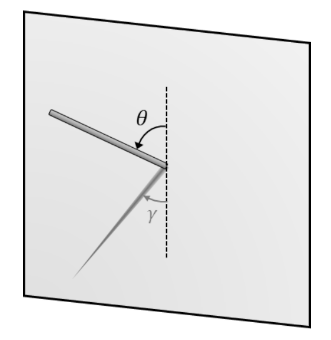
\includegraphics{imagens/q20.png}
        \caption{Esquema relógio de Sol.}
    \end{figure}
    \begin{alternativas}
        \item Suponha um relógio de Sol vertical cujo gnômon esteja corretamente apontado para o sul.
        Seja \(\phi\) a latitude do observador, \(H\) o ângulo horário do Sol e \(\delta\) a declinação solar. Determine
        a relação entre \(\theta\) e \(\gamma\) em função dessas variáveis.
        \item  Com base no item anterior, qual deve ser o valor de \(\theta\) para que o relógio funcione o ano todo?
        \item  Utilizando o valor correto para \(\theta\), determine a relação entre \(\gamma\) e \(H\), em função apenas de \(\phi\).
    \end{alternativas}
\end{pproblem}

\pts{2} 
\begin{pproblem}
    Qual a menor altura que um gigante (que vive MUITOS), localizado no polo Sul, precisa ter para conseguir ver todas as estrelas do céu?

\begin{pssolution*}
    O ângulo abaixo do horizonte que o gigante consegue enchergar, é dado por, 


    \[\cos\theta = \frac{R_\oplus}{R_\oplus + H}\]

    Onde \(H\) é a altura do gigante. Devido a presseção dos equinónicos, o polo sul ficará "\(23,47^\circ\) para cima" na ecliptica, logo, o ângulo do horizonte deve ser \(\theta = 90^\circ -23,47^\circ = 66,53^\circ\) . Resolvendo para \(H\), temos, 

    \[\boxed{H = R_\oplus\left(\frac{1}{\cos\theta}-1\right) \approx 9,62\cdot 10^6\text{ m}}\]
\end{pssolution*}
\end{pproblem}


\pts{3}
\begin{pproblem}
    Toleduardo deseja ver o por do Sol, mas acabou passando tempo de mais na SorveterITA. Toleduardo é um homem \textit{Just in time} e deseja saber quanto tempo o por do Sol vai durar, para que ele possa se atrasar com calma. Sabendo que o Toleduardo só vai para a SorveterITA dias 21 de março ou 22 de setembro, calcule qual a duração do por do Sol na SorveterITA.
    \\
    \textbf{Dados: } Latitude da SorveterITA \(\phi = 23^\circ \ 10' \ 45''S, \ \ \lambda = 45^\circ 53' 14''O\).
\end{pproblem}


\pts{3}
\begin{pproblem} (Lista 2 - Vinhedo 2021)
    Em fevereiro de 2015, a Lua começou um ciclo de ocultações mensais de Aldebaran ($\alpha$ Tau). Ou seja, todo mês a Lua passava na frente de Aldebaran para um observador na Terra. Vale ressaltar que essas ocultações não ocorriam necessariamente para observadores na mesma posição todo mês. 

    Calcule a data (mês e ano) do fim desse ciclo de ocultações mensais. Considere que a órbita da Lua é circular.

    \subsection*{Dados:}

    \begin{itemize}
        \item Latitude eclíptica de Aldebaran = $5,47^\circ$
        \item Período de precessão nodal da Lua = 18,6 anos
    \end{itemize}

\end{pproblem}


\pts{4}
\begin{pproblem} (Lista 2 - Vinhedo 2021)
    Miguel vive em uma ilha isolada no oceano Pacífico Sul, em uma longitude
    $\lambda = 176^{\circ}09^{\prime}137,7^{\prime\prime}\text{W}$. Ao longo do ano, o local onde o Sol nasce visto por Miguel varia $\Delta A = 67^{\circ}03^{\prime}81^{\prime\prime}$ no horizonte. Para os dois primeiros itens, desconsidere a refração atmosférica. Com essas informações, descubra:

    \begin{alternativas}
        \item A latitude $\phi$ e o nome da ilha. (Consulte o Google Earth ou software similar)
        \item O intervalo de horários em que o Sol nasce na ilha, dado o fuso horário peculiar $UT + 12\frac{3}{4}$.
        \item Considerando a refração atmosférica, o tamanho do intervalo do item anterior iria diminuir, aumentar ou se manter constante?
    \end{alternativas}

\end{pproblem}

\pts{3}
\begin{pproblem}(Lista 2 - Vinhedo 2022) 
    Bruno decidiu alugar uma casa para passar as férias em Cuiabá ($15,3^{\circ} \text{S}$, $56,1^{\circ} \text{O}$). Como um bom astrônomo, Bruno passava suas noites sentado em uma cadeira observando as estrelas por uma gigante porta voltada para o ponto cardeal sul.

    A porta tinha 4,00 metros de altura e 1,50 metros de largura. Bruno tinha o costume de sentar a
    1,00 metro da porta perfeitamente alinhado com o seu centro na horizontal. Ou seja, o segmento
    de reta entre os olhos de Bruno e o ponto que está exatamente no meio da porta na horizontal e
    na altura dos olhos forma um ângulo de $90^{\circ}$ com o plano da porta. Os olhos de Bruno ficam a
    1,20 metros do chão quando ele está na cadeira.
    
    Para facilitar as suas observações, Bruno criou um sistema de coordenadas baseado na posição da
    porta onde ele via as estrelas a partir do local onde ele estava sentado, utilizando metros como
    a unidade de referência. A origem do sistema está no canto inferior esquerdo. As coordenadas
    em $x$ aumentam para a direita e as coordenadas em $y$ aumentam para cima. Dessa forma, uma
    estrela vista a 1 metro do lado esquerdo da porta e 2 metros acima do chão seria representada
    pelas coordenadas $(1, 2)$.
    
    Bruno estava bastante interessado em Shaula ($\lambda \ \text{Sco}, \delta = 37,1^{\circ} \text{S}$). Determine as coordenadas de
    Shaula no instante em que a estrela se tornava visível para Bruno quando observada através da
    porta. Assuma que Shaula estava abaixo do horizonte quando Bruno começava a observar o céu.
    
\end{pproblem}


\newpage

\section{Fotometria e Física Moderna}

\pts{3} 
\begin{pproblem}
    O objetivo dessa questão é deduzir uma expressão para a \textit{profundidade óptica}. Imagine que um feixe de luz passe por uma região do espaço, com uma determiada quantidade de partículas. Se \(I_0\) é a intensidade da luz antes de passar por tal região de espaço e \(I\) é a intensidade da luz após, a profundidade óptica é definida como:
    \[I = I_0e^{-\tau}\]
    Onde \(\tau\) é a profundidade óptica.
    \\
    Considere uma região do espaço possuí densidade numérica de partículas \(n\).
    \begin{alternativas}
        \item Qual o número de partículas em uma área \(A\) e espessura \(dz\)?
        \item Supondo que cada partícula possua sessão transversal \(\sigma\), qual é a área tampada pelas parículas?
        \item Encontre a fórmula para \(\tau\). 
    \end{alternativas}

\begin{pssolution*}{}{}
    \begin{alternativas}
        \item A densidade volumétrica de partículas é \(n\), sendo assim temos que o número \(dN\) de partículas em um volume \(dV\) é dado por
        \[\boxed{dN = ndV \equiv nAdz}\]

        \item Se cada particula ocupa uma área \(\sigma\), a área ocupada por \(dN\) particulas é
        \[\boxed{dS = \sigma dN = \sigma nAdz}\]

        \item É esperado que a área ocupadas pelas particulas seja um empecilho para a passagem da luz. Como a Intensidade é proporcional a área disponível para a passagem da luz, nós temos
        \[\frac{dI}{I} = -\frac{dS}{A} = -n\sigma dz\]
        Integrando, obtemos

        \[I = I_0 e^{-n\sigma z}\]

        Ou seja, 

        \[\boxed{\tau = n\sigma z}\]
    \end{alternativas}
\end{pssolution*}
\end{pproblem}

\pts{2}
\begin{pproblem} A Galáxia do Triângulo, \(M33\), é a terceira maior galáxia do grupo local, ela está a uma distância \(d=970 \text{ kpc}\) de nós e possuí magnitude aparente de \(5,72\). Sabendo que ela possuí aproximadamente \(40\) bilhões de estrelas, encontre a luminosidade média das estrelas de \(M33\). Sua estimativa parece condizer com a realidade? Por que?
\begin{pssolution*}{}{}
    Utilizando a equação de Pogson

    \[m-M_\odot = -2,5\log \left(\frac{L_{g}}{L_\odot}\left(\frac{10 \text{ pc}}{d}\right)^2\right)\]

    Resolendo para \(L_g\), 

    \[L_g = L_\odot \left(\frac{d}{10\text{ pc}}\right)^2 10^{-0,4(m-M_\odot)}\]

    Temos também, que \(L_g = \overline{L_\star} N\) e assim

    \[\overline{L_\star} = \frac{L_\odot}{N} \left(\frac{d}{10\text{ pc}}\right)^2 10^{-0,4(m-M_\odot)}\]

    Utilizando os valores da tabela de constantes, obtemos:

    \[\overline{L_\star} \approx 0,1L_\odot\]

    No entando, essa estimativa não condiz com a realidade, uma vez que há fatores como a extinção interestelar que contribuem para o aumento da magnitude aparente de \(M33\), uma estimativa condizente estaria na mesma ordem de grandeza da Luminosidade do Sol.

\end{pssolution*}
\end{pproblem}

\pts{4}
\begin{pproblem}
    Considere que o universo possuí densidade numérica de estrelas, isto é, numero de estrelas por unidade de volume, constante e de valor \(n\). Assumindo que todas elas tenham \(L = L_\odot\) e que existam um total de \(N_0\) estrelas no universo.
    
    \begin{alternativas}
    \item qual a probrabilidade da magnitude absoluta de uma estrela, vista do centro do universo, ter magnitude entre \(m\) e \(m+dm\), onde \(dm\) é uma porção infinitesimal de magnitude? Deixe sua resposta em termos de \(m\) e da maior magnitude possivél, \(m_{lim}\), de uma estrela na "borda" do universo.

    \item Qual a probabilidade de uma estrela poder ser observada a olho nu?
    
    \textbf{Dados:} \[\int_{-\infty}^{6}10^{0,6(x-A)}dx \approx 2881.6 e^{-1.381 A}\]
    \end{alternativas}\begin{pssolution*}{}{}
    \begin{alternativas}
    \item A magnite aparente de uma estrela é dada por, 

    \[m = -2,5\log F + C\]

    Onde \(C\) é uma constante. Escrevendo \(F = L/4\pi r^2\), temos, 

    \[m = -2,5\log\left(\frac{L}{4\pi r^2}\right) + C = 5\log r -2,5 \log \left(\frac{L}{4\pi}\right)+ C\]

    Mas como \(L\) é constante para todas as estrelas, podemos absorver o segundo termo para a constante. Assim, 

    \[m=5\log r + C \rightarrow r = 10^{0,2(m-C)}\]

    Derivando a expressão de \(m\), temos, 

    \[\frac{dm}{dr} = \frac{5}{r\ln 10}\]

    Agora, vamos achar a probabilidade de uma estrela estar a uma distância \(r\).

    O numero de estrelas contidas entre \(r\) e \(r+dr\) é 

    \[dN(r) = 4\pi n r^2dr\]

    Dividindo por \(N_0\), temos que a probabildiade de uma estrela estar nessa distância é 

    \[dP(r) = \frac{dN(r)}{N_0} = \frac{4\pi n r^2}{N_0}dr \rightarrow dr = \frac{N_0}{4\pi n r^2} dP(r)\]

    Substituindo a expressão para \(dr\), 

    \[\frac{r\ln 10}{5}dm = \frac{N_0}{4\pi n r^2}dP(r)\]

    Isolando \(dP(r)\), 

    \[dP(r) = \frac{4\pi \ln 10 n r^3}{5 N_0}dm\]

    Substituindo a expressão de \(r\), podemos realizar a mudança de variável \(r\rightarrow m\)em \(dP\)

    \[dP(m) = \frac{4\pi n \ln 10  }{5 N_0}10^{0,6(m-C)}dm\]

    Para achar o valor de \(C\), vamos comparar com a magnitude limite, na "borda" do universo. Como o universo possuí \(N_0\) estrelas, seu raio deve ser dado por, 

    \[N_0 = \frac{4\pi R^3}{3} \rightarrow R = \left(\frac{3N_0}{4\pi}\right)^{1/3}\]

    Equacionando agora para \(m_{lim}\), 
    
    \[m_{lim} = 5\log R + C\]

    No qual, podemos isolar a constante \(C = m_{lim}-5\log R\). Substituindo na expresssão de \(dP(m)\),

    \[dP(m) = \frac{4\pi n \ln 10  }{5 N_0}10^{0,6(m-m_{lim}+5\log R)}dm\]

    Trabalhando nessa expressão, 

    \[dP(m) = \frac{4\pi n \ln 10  }{5 N_0}10^{0,6(m-m_{lim})}10^{3\log R}dm\]

    Usando as propriedades do log, \(a\log b = \log b^a\) e \(10^{\log x} = x\), temos, 

    \[dP(m) = \frac{4\pi n R^3\ln 10}{5N_0}10^{0,6(m-m_{lim})}dm\]

    Substituindo \(R\), 

    \[\boxed{dP(m) = \frac{3\ln 10}{5}10^{0,6(m-m_{lim})}dm}\]

    Ou seja, a probabilidade não depende de \(n\) e nem de \(N_0\)!

    \item Para uma estrela ser vísivel, sua magnitude deve ser \(m\leq 6\), assim, equacionando, 
    
    \[P(m\leq 6) = \int_{-\infty}^6 dP(m) = \frac{3\ln 10}{5}\int_{-\infty}^610^{0,6(m-m_{lim})}dm\]

    Usando a integral dada no enuncicado, 

    \[P(m\leq 6) = \frac{3\ln 10}{5}2881,6 e^{-1,381 m_{lim}}\]

    Simplificando os fatores numéricos, 

    \[\boxed{P(m\leq 6) \approx 3981,08 e^{-1,381 m_{lim}}} \]

    A fim de curiosidade, colocando \(m_{lim}\approx 40\), para uma estimativa, teriamos, 

    \[P(m\leq 6)\approx 10^{-20}\]

    Ou seja, mesmo no modelo mais simples o universo, a nossa capacidade e insigficicancia prevalece.
    \end{alternativas}

\end{pssolution*}
\end{pproblem}

\pts{4}
\begin{pproblem}
    O \textit{Brilho Superfícial}, fluxo por ângulo sólido por frequência, \(B_\nu\) é dada pela Lei de Plank:
    \[B_\nu = \frac{dF}{d\nu d\Omega} = \frac{2h\nu^3}{c^2(e^{\frac{h\nu}{k_BT}}-1)}\] 
    \begin{alternativas}
        \item Encontre uma expressão para:
        \[B_\lambda = \frac{dF}{d\lambda d\Omega}\]
        \item A partir de \(B_\lambda\) encontre o comprimento de onda máximo de onda \(\lambda_{max}\) que uma estrela de temperatura \(T\) emite (você terá que resolver algo numéricamente).
        \item Para pequenas frequências temos a aproximação de Righlight-Jeans. Obetenha uma expressão para \(B_\nu\) para frequêncais pequenas.
        \end{alternativas}

\begin{pssolution*}{}{}
    \begin{alternativas}
        \item Temos que
        \[B_\lambda = \frac{dF}{d\lambda d\Omega} = \frac{dF}{d\nu d\Omega}\frac{d\nu}{d\lambda}\]

        Utilizando a relação fundamental da ondulatória, \(c=\nu\lambda \rightarrow \nu = c/\lambda\) chegamos em 

        \[B_\lambda = \frac{2h(c/\lambda)^3}{c^2(e^{\frac{hc}{\lambda k_BT}}-1)}\frac{d}{d\lambda}\left(\frac{c}{\lambda}\right) = \frac{2hc^2}{\lambda^5}\frac{1}{(e^{\frac{hc}{\lambda k_BT}}-1)}\]

        \item Para resolver esse item, pracisamos achar o ponto máximo de \(B_\lambda\). Mas diferenciar \(B_\lambda\) diretamente é uma tarefa estremamente chata. Uma ideia mais eficiente é tirar o logaritimo natural de \(B_\lambda\) e diferenciar o mesmo. Uma vez que estamos no ponto de máximo, ambas as maneiras chegarâo no mesmo, resultado
        
        \[\ln B_\lambda = -5\ln \lambda - \ln (e^{hc/\lambda k_BT}-1) + C\]

        Onde \(C\) é uma constante que absorve os \(\ln\) das outras constantes de  \(B_\lambda\). Continuando a derivar 

        \[\frac{d \ln B_\lambda}{d\lambda} = -\frac{5}{\lambda} + \frac{e^{hc/\lambda k_BT}}{e^{hc/\lambda k_BT}-1}\frac{hc}{k_BT\lambda^2}=0\]

        Definindo \(x = \frac{hc}{k_BT\lambda}\) 

        \[\frac{xe^x}{e^x-1}=5\]

        \[x=5e^{-x}(e^x-1) = 5(1-e^{-x})\]

        Utilizando iteração, podemos resolver para \(x\), obtendo \(x\approx 4,965\). Voltando a definição de \(x\)

        \[4,965 = \frac{hc}{k_B T\lambda_{max}}\rightarrow \boxed{\lambda_{max} \approx \frac{2,989 \cdot 10^{-3}}{T}}\]

        Essa é a famosa \textit{Lei de Wien}, comumente escrita na forma \(\lambda = b/T\), onde \(b\approx 2,989 \cdot 10^{-3}\).

    \end{alternativas}
\end{pssolution*}
\end{pproblem}

\pts{3}
\begin{pproblem}
    A luminosidade de um corpo secundário, depende da área iluminada vísivel do astro. Nestá questão vamos fazer um breve estudo sobre esse fenômeno.
    \begin{alternativas}
        \item  Considere a Seguinte situação:
        \begin{figure}[H]
            \centering
            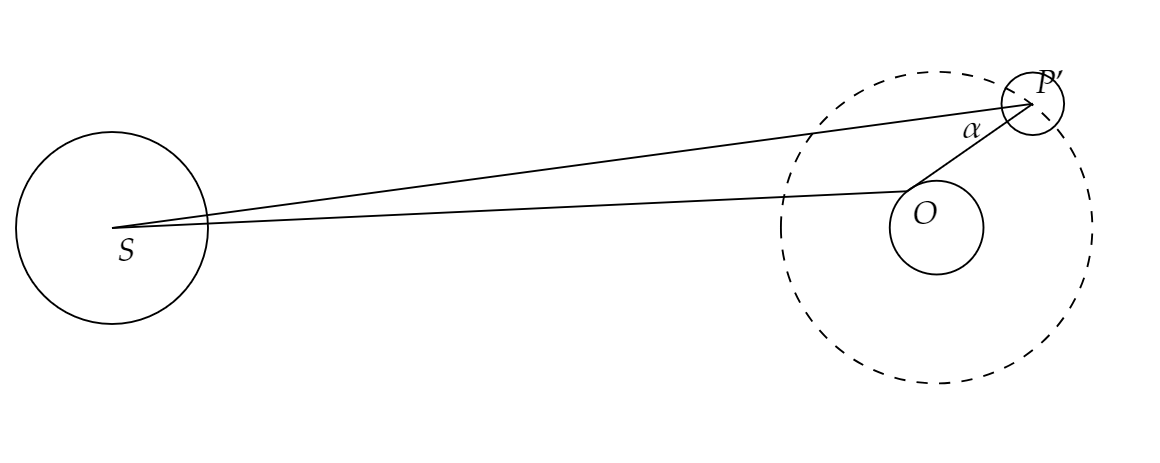
\includegraphics[width=0.8\linewidth]{imagens/fotometria 1.png}
            \caption{Esquema Sol-Terra-Lua}
        \end{figure}

        Encontre uma expressão para a razão \(\Phi\) entre a área iluminada em função de \(\alpha\) e a área total do planeta.
        
        \item Encontre os ângulos \(\alpha\) em que temos a fase da Lua em: Nova, crescente, cheia e minguante, respectivamente.
    \end{alternativas}

\begin{pssolution*}{}{}
    Para resolver a questão, vamos nos guiar no esquema da imagem abaixo:
    \begin{figure}[H]
       \centering
       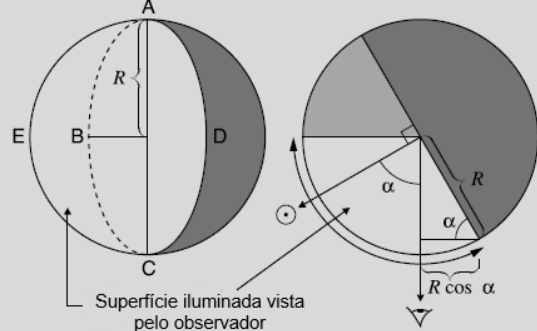
\includegraphics[width=0.8\linewidth]{imagens/fotometriaplanetaria.png}
       \caption{Fonte: Introduction do Planetary Fotometry} 
    \end{figure}

    Do lado esquerdo, vamos um esquema de como o plaeta se parece no céu e na direita uma representação vista "de cima". Aqui, podemos perceber que a área que vemos é composta por metade da área do cículo mais metadade da área de uma elipse de semi eixo maior \(R\) e semi eixo menor \(R\cos\alpha\). Assim

    \[\Phi = \frac{\pi R^2/2 + \pi R^2\cos\alpha/2}{\pi R^2} \ \boxed{\therefore \Phi = \frac{1+\cos\alpha}{2}}\]

    Na Lua nova, temos \(\Phi = 0\), na crescente \(\Phi = 1/2\), na cheia \(\Phi = 1\) e na minguante \(\Phi = 1/2\), assim:

    \[\boxed{\alpha_{nova} = 180^\circ, \ \alpha_{crescente} = 90^\circ, \ \alpha_{cheia} = 0^\circ, \ \alpha_{minguante} = 90^\circ}\]
\end{pssolution*}
\end{pproblem}

\pts{5}
\begin{pproblem} (Apostila Magna)
    Neste problema, modelaremos o efeito da atmosfera na Terra. Suponha que o Sol
seja um corpo negro de temperatura \(T_1\) e raio \(R_1\). A Terra é uma esfera que está localizada
a uma distância \(R\) do Sol e possui raio \(R_3\). A emissividade da Terra é \(\epsilon_3\).
\begin{alternativas}
    \item Se não houvesse atmosfera na Terra, determine sua temperatura de equilíbrio, \(T_3\).
    \item  Agora, consideraremos os efeitos da atmosfera. Modele-a como uma casa esférica de gás,
    com uma emissividade \(\epsilon_2\) e raio exterior \(R_2>R_3\), concêntrica à Terra. No equilíbrio térmico,
    sua absortividade para os comprimentos de onda no ultravioleta e no infravermelho é \(\epsilon_2\). A
    atmosfera transmite uma fração \(t\) da radiação ultravioleta mas é completamente opaca ao
    infravermelho. Assumindo que o Sol emita luz ultravioleta enquanto a Terra emite e re-emite
    no infravermelho, determine as temperaturas \(T_2\) da atmosfera e \(T_3\) da Terra, no equilíbrio
    termodinâmico. Assuma que a atmosfera seja um condutor de calor perfeito, de forma que
    toda a radiação incidente sobre ela seja uniformemente distribuída por sua superfície.
\end{alternativas}

\begin{pssolution*}{}{}
    \begin{alternativas}
        \item No equilíbiro termodinâmico, temos que a quantidade de potencia absorvida é a mesma que a emitida. Além disso, a emissividade e a absortividade são as mesmas. Desse modo, 
        \[\frac{4\pi R_1^2\sigma T_1^4}{4\pi R^2}\pi R_3^2\epsilon_3 = 4\pi R_3^2\sigma T_3^4\epsilon_3\]

        Resolvendo para \(T_3\), 

        \[\boxed{T_3 = T_1\left(\frac{R_1^2}{4\pi R^2}\right)^{1/4}}\]

         \item A temperatura da atmosfera é calculada por 
         
         \[T_2 = T_1\left(\frac{R_1^2}{4\pi R^2 }\right)^{1/4}\]

         O processo é analogo ao item anterior. A luminosidade transmitida pela terra é, 

         \[L_2 = {4\pi R_2^2\sigma T_2^4\epsilon_2} t\]

         A Terra irá refletir toda essa radiação e a atmosfera refletirá de volta apenas uma fração t, desse modo, a luminosidade total é dadda por, 

         \[L_{2,T} = 4\pi R_2^2\sigma T_2^4\epsilon_2 (t+t^2+t^3+...)\]

         O item dentro do parenteses é uma somatóriso de PG infinito, com \(q_1 = t\) e \(r = t\), como \(t<1\), o valor do somatório vale, 

         \[(t+t^2+t^3+...) = \sum_{n=1}^{\infty}t^n = \frac{t}{1-t}\]

         Igualando ambas, 

         \[L_{2,T} = L_3 \rightarrow \frac{4\pi R_2^2\sigma T_2^4 \epsilon_2 t}{1-t} = 4\pi R_3^2\sigma T_3^4\]

         Resolvendo para \(T_3\), 

         \[T_3 = T_2\left(\frac{R_2^2\epsilon_2}{R_3^2}\frac{t}{1-t}\right)^{1/4}\]

         Substituindo o valor de \(T_2\), 

         \[\boxed{T_3 =T_1\left(\frac{R_1^2R_2^2}{4\pi R^2R_3^2}\frac{\epsilon_2t}{1-t}\right)^{1/4}}\]


    \end{alternativas}
    
\end{pssolution*}
\end{pproblem}


\pts{2}
\begin{pproblem}(Lista 2 - 2021)
    A Nebulosa do Anel (M57) possui uma magnitude aparente igual a 9 e um
diâmetro angular de 2$^{\prime}$ para um observador na Terra. Qual seria a magnitude aparente do céu
noturno de um planeta orbitando uma estrela exatamente no centro de M57?
\begin{pssolution*}{}{}
    O céu noturno compreende um ângulo sólido de \(2\pi\) sr, já o ângulo sólido visto por nés é \(\Omega \approx \pi \theta^2\), onde \(\theta\) é o raio angular. Como o Fluxo é proporcional a \(\Omega\), temos

    \[m_{ceu}-m = -2,5\log\left(\frac{\Omega_{ceu}}{\Omega}\right)\]

    Para converter \(\Omega\) de arco-minuto\(^2\) para sr, temos que multiplicar por \(\left(\frac{\pi}{180\cdot60}\right)^2\), assim
    
    \[m_{ceu} = 9 - \log\left(\frac{2\pi}{\pi(\frac{\pi}{180\cdot60})^2}\right)\]

    \[\boxed{m_{ceu} = -9,43}\]
\end{pssolution*}
\end{pproblem}


\pts{4}
\begin{pproblem} (Adaptado Lista 4 - 2021)
    O Efeito Cherenkov foi primeiramente detectado pelo cientista soviético
    Pavel Cherenkov, em 1937. Mais tarde, em conjunto com seus colegas de trabalho, I. E. Tamm e
    I. M. Frank, ele interpretou fisicamente o fenômeno, ganhando, assim, o Prêmio Nobel de Física
    de 1958. Antes de fazer um estudo matemático, precisamos, primeiro, entender um pouco mais
    sobre seu princípio.

    Quando partículas carregadas de alta energia percorrem um meio dielétrico, é possível que, caso
    sua velocidade seja maior que a velocidade de fase ($\frac{c}{n}$), átomos sejam excitados. Esses, por sua
    vez, ao retornarem ao estado fundamental, emitem radiação eletromagnética. As ondas emitidas
    se espalham de forma esférica e, quando somadas, formam um cone de ângulo de abertura $2\alpha$,
    como mostra a figura abaixo.
    \begin{figure}[H]
      \centering
      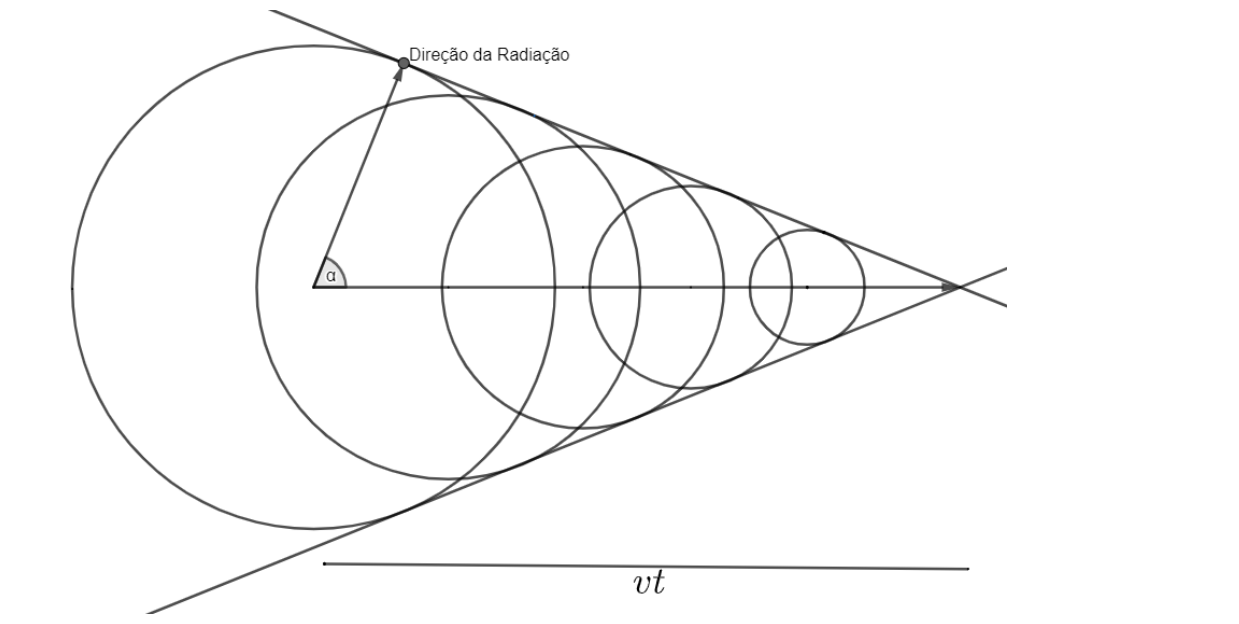
\includegraphics[width=0.9\linewidth]{imagens/cherenkov.png}  
      \caption{Mecanismo de radiação do Efeito Cherenkov}
    \end{figure}

    Esse efeito é similar a um jato movendo-se em velocidade supersônica, ou seja, segue o mesmo
    princípio do Cone de Mach, porém, com a luz. Finalmente, iremos desenvolver o modelo matemático do Efeito Cherenkov.

    \begin{center}
        \textbf{Parte A - Modelo Teórico}    
    \end{center}
    
    Considere uma partícula movimentando-se a velocidades relativísticas em um meio de índice de
    refração $n$. Sabe-se que sua massa de repouso é $m_0$, possui momento linear $p$ e velocidade $v$. Em
    determinado momento, há emissão de um fóton sob um ângulo $\alpha$, como mostra a figura 1.

    \begin{alternativas}
        \item Sendo $\mu$ a frequência do fóton emitido, determine a equação de seu momento
        linear, $p_\mu$, e sua energia, $E_\mu$. Sua resposta deve estar em função de $n$, $\mu$ e constantes físicas.
        \item Encontre uma expressão para o momento linear da partícula após a emissão
    do fóton em função de $p_\mu$, $p$ e $\alpha$.
        \item Sendo $\beta_n = \frac{c}{vn}$, prove que a relação abaixo é verdadeira:
        \begin{equation}
            \cos\alpha = \frac{1}{\beta_n}
        \end{equation}
        \item Considerando que o momento linear e a energia se conservem, determine a
        velocidade mínima para a ocorrência do Efeito Cherenkov.
        \textbf{Dica:} Quando comparado com os outros parâmetros, o fator $(n^2-1)h\mu$ pode ser desprezado.

    \begin{center}
        \textbf{Parte B - Reações Nucleares}    
    \end{center}
    
    A cadeia próton-próton é um processo de reações de fusão para conversão de hidrogênio em hélio.
    Um dos ramos possíveis da cadeia próton-próton é a $pp \text{ IV}$, na qual, teoricamente, um átomo de
    hélio-3 reage diretamente com um próton, conforme a reação a seguir:

    \begin{equation}
        ^3\text{He} + ^1\text{H} \rightarrow ^4\text{He} + \nu + \_\_
    \end{equation}

        \item  Indicando a lei de conservação nuclear utilizada, indique qual partícula faltante
        no quadrado da reação acima.

        \item  Indicando a lei de conservação nuclear utilizada, indique qual partícula faltante
        no quadrado da reação abaixo:

        \begin{equation}
            \pi^- \rightarrow \mu^- + \_
        \end{equation}
        
        \textbf{Dados:} Massa do píon: $140 \ \text{MeV}/c^2$, massa do múon: $106 \ \text{MeV}/c^2$.
    \end{alternativas}

\begin{pssolution*}{}{}
    \begin{center}
        \textbf{Parte A - Modelo Teórico}    
    \end{center}

    \begin{alternativas}
        \item Para um fóton, as relações de De Broglie, nos dizem que 
        \[E = h\mu, \ \ p = \frac{h}{\lambda}\]
        Onde \(h\) é a constante de plank.

        Utilizando a relação fundamental da ondulatória, \(\lambda = v/\mu = \frac{c}{n\mu}\), assim 

        \[\boxed{E = h\mu, \ \ p = \frac{nh\mu}{c}}\]

        \item Como o momento total é conservado, considereque a particula está se movendo com momento \(p\) ao longo do eixo \(x\), antes de emitir um foton. Assim, temos 
        
        \[p = p_\mu\cos\alpha + p'_x\]

        \[p_\mu\sin\alpha = p'_y\]

        \[p' = \sqrt{p_x^2 + p_y^2}\]

        Resolvendo para \(p'\)

        \[p'^2 =(p - p_\mu\cos\alpha)^2 +p_\mu^2\sin^2\alpha \]

        \[p'^2 = p^2 - 2p_\mu p \cos\alpha + p_\mu^2\]

        Finalmente

        \[p' = \sqrt{p^2-2pp_\mu\cos\alpha+p^2_\mu}\]

        \item Olhe a seguinte figura, 
        
        \begin{figure}[H]
            \centering
            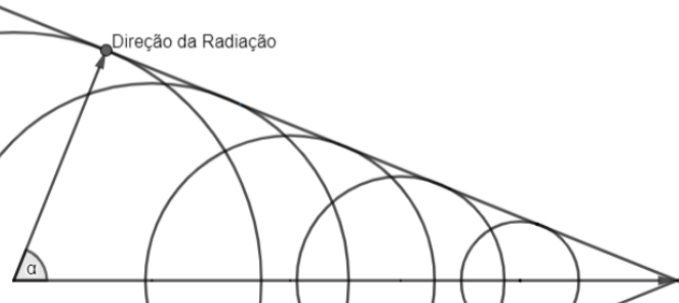
\includegraphics[width=0.7\linewidth]{imagens/cherenkov.1.png}
            \caption{Esquema Cherenkov}
        \end{figure}

        Note que o raio do circulo é dado pela distância percorrida pelo fóton. A distância percorrida do centro do cirulo até o fim do cone é \(vt\), assim

        \[\boxed{\cos\alpha = \frac{ct}{nvt} = \frac{c}{nv} \equiv \frac{1}{\beta_n}}\]

        \item Definindo \(c=1\), a conservação de energia nos diz
        \[\sqrt{p^2+m_0^2} = \sqrt{p'^2+m_0^2}+h\mu\]

        Trablhando nessa expressão

        \[\sqrt{p'^2 + m_0^2} = \sqrt{p^2+m_0^2} - h\mu\]

        \[p'^2 + m_0^2 = p^2+m_0^2 + h^2\mu^2 - 2h\mu\sqrt{p^2+m_0^2}\]

        Substituindo \(p'\)

        \[p^2-2pp_\mu\cos\alpha+p^2_\mu = p^2+h^2\mu^2 - 2h\mu\sqrt{p^2+m_0^2}\]

        Resolvendo para \(\cos\alpha\) 

        \[\cos\alpha = \frac{p_\mu^2 - h^2\mu^2+2h\mu\sqrt{p^2+m_0^2}}{2pp\mu}\]

        Simplificando 

        \[\cos\alpha = \frac{p_\mu}{2p} - \frac{h^2\mu^2}{2pp_\mu} + \frac{h\mu\sqrt{p^2+m_0^2}}{pp_\mu}\]
        
        Substituindo \(p_\mu = nh\mu\)

        \[\cos\alpha = \frac{nh\mu}{2p} + \frac{h\mu}{2np}+ \frac{\sqrt{p^2+m_0^2}}{np}\]

        \[\cos\alpha = \frac{h\mu(n^2-1)+2\sqrt{p^2+m_0^2}}{2np}\]

        Desprezando o termo \(h\mu(n^2-1)\) e substituindo \(\cos\alpha\)

        \[\frac{1}{nv} = \frac{\sqrt{p^2+m_0^2}}{np}\]

        Resolvendo para \(v\)

        \[v = \frac{p}{\sqrt{p^2+m_0^2}}\]

        Porfim, voltando os \(c\)'s, temos 

        \[\boxed{v = \frac{pc^2}{\sqrt{p^2c^2+m_0^2c^4}}}\]

        \begin{center}
            \textbf{Parte B - Reações Nucleares}    
        \end{center}

        \item Utilizando a conservação de carga, do lado esquerdo temos \(2+1=3\) prótons, porém do lado direito, só temos \(2\), portanto a particula faltante deve conter um proton. Já a massa atômica, segue como \(3+1=4\) e do lado direito \(4\). Assim, a particula faltante deve ter a carga de um proton e a massa muito menor do que este. A única partícula que seja essa descrição é o \(\boxed{\text{pósiton, }e^+}\).
            
        \item Utilizando que o número leptônico é constante, temos que o pion não é um lepton \(n_L=0\), mas o múon, é um lepton com \(n_L=+1\), então a nossa partícula deve ter \(n_L=-1\). O únio antilépton neutro associado ao múon com \(n_L=-1\) é o antineutrino do múon, \(\bar{\nu}_\mu\), portanto, a relação completa é 
        \[\boxed{\pi^{-}\rightarrow \mu^- + \bar{\nu}_\mu}{}\]

    \end{alternativas}

\end{pssolution*}
\end{pproblem}


\pts{3} 
\begin{pproblem}(Lista 3 - Vinhedo 2022)
Juvelino, diretamente de seu observatório em Paris, França, monitora a estrela Polaris ($\alpha\text{UMi}$). Ele tem como objetivo descobrir a temperatura de cor $T_c$ do astro. Alguns dos dados de que ele dispõe a respeito de seu alvo são:

\begin{itemize}
    \item Magnitude aparente na banda $V$: $V = 1,98$;
    \item Magnitude absoluta na banda $V$: $M_V = -3,60$;
    \item Magnitude absoluta na banda $B$: $M_B = -3,19$.
\end{itemize}

Com as informações fornecidas, ajude Juvelino!

\begin{alternativas}
    \item Realizando diversas observações, Juvelino determinou que a extinção interestelar na banda $V$ na direção de Polaris é $a_V = 5,8 \, \text{mag/kpc}$. Determine a distância, em pc, de $\alpha\text{UMi}$ até a Terra.
    \item Usando a relação empírica
    \begin{equation}
        \frac{A_V}{E_{B-V}} = 3,0
    \end{equation}
    sendo $A_V$ a extinção interestelar total na banda $V$ e $E_{B-V}$ o excesso de cor $B-V$, determine o índice de cor $B-V$ da estrela observada.
    \item Demonstre a relação
    \begin{equation}
        T_c = \frac{7009}{(B-V) + 0,47}
    \end{equation}
    na qual a temperatura de cor é dada em Kelvin. Para tanto, use o fato de que estrelas de classe espectral $A0$ possuem $(B-V) = 0$ e $T_c = 15000 \, \text{K}$. Use também que os comprimentos de onda das bandas $B$ e $V$ são, respectivamente, $\lambda_B = 440 \, \text{nm}$ e $\lambda_V = 548 \, \text{nm}$. Justifique quaisquer aproximações feitas.

    \textbf{DICA: A lei de plack talvez seja útil}
    \item Determine a temperatura de cor de Polaris.
\end{alternativas}
\begin{pssolution*}{}{}
    \begin{alternativas}
        \item A expressão que relaciona corretamente as magnitudes é 
        \[V - M_V = 5 \log d - 5 + a_V d\]

        Essa equação, só pode ser resolvida por meio da iteração,

        \[d = \frac{V-M_V - 5\log d + 5}{a_v}\]

        Iterando, chegamos em \(\boxed{d\approx 100\text{ pc}}\).

        \item Pela definição, \(E_{B-V} = A_B - A_V\). Assim
        
        \[\frac{A_V}{A_B-A_V} = 3,00\]

        \[A_B = \frac{A_V}{3}+A_V = 0,77\]

        Assim, 

        \[B-M_B = 5\log d - 5 + A_B\rightarrow B = 2,58\]

        E pela definição, o índice \(B-V\) = \(\boxed{U_{B-V} = B-V = 0,60}\)

        \item Utilizando a Lei de Planck, temos que 
        
        \[\frac{B_B}{B_V} = \frac{F_B}{F_V} \left(\frac{\lambda_V}{\lambda_B}\right)^5 \frac{e^{\frac{\beta hc}{\lambda_V}-1}}{e^{\frac{\beta hc}{\lambda_B}-1}}\]

        Utilizando a aproximação de Wein, temos

        \[\frac{F_B}{F_V} = \left(\frac{\lambda_V}{\lambda_B}\right)^5 \frac{e^{\frac{\beta hc}{\lambda_V}}}{e^{\frac{\beta hc}{\lambda_B}}}\]

        Utilizando a equação de Pogson para comparar as magnitudes, 

        \[B-V = -2,5\log\left(\frac{F_B}{F_V}\right)+C\]

        Aqui adicionamos uma constante, pois estamos trabalhando com diferentes comprimentos de ondas. Trabalhando na expressão, 

        \[B-V = -2,5\log\left(\left(\frac{\lambda_V}{\lambda_B}\right)^5 \frac{e^{\frac{\beta hc}{\lambda_V}}}{e^{\frac{\beta hc}{\lambda_B}}}\right)+C\]

        Trabalhando nessa expressão, 

        \[B-V = -2,5\log\left(\frac{\lambda_V}{\lambda_B}\right)^5 + 2,5 \beta hc\left(\frac{1}{\lambda_B}-\frac{1}{\lambda_V}\right)\log e + C\]

        E utilizando \(\beta = \frac{1}{k_B T_c}\) e substituindo os valores, 

        \[B-V = -1,19 + \frac{7009}{T_c}+C\]

        Para o tipo \(A_0\), \((B_V)=0\) e \(T_c = 15000\)K. Assim, 

        \[-1,19 + \frac{7009}{15000} + C = 0 \rightarrow C = 0,72\]

        Assim, 

        \[B-V = -0,47 + \frac{7009}{T_c} \rightarrow \ \ \boxed{T_c = \frac{7009}{(B-V) + 0,47}}\]

        \item da equação anterior, 
        
        \[\boxed{T_c = \frac{7009}{0,60 + 0,47} \approx 6600 \text{ K}}\]
    \end{alternativas}    

\end{pssolution*}
\end{pproblem}


\newpage

\section{Termodinâmica}
\pts{3}
\begin{pproblem}
    Uma galáxia possuí na ordem de \(10^{10}\) estrelas, por essa quantidade imensa, podemos modelar uma galáxia como sendo uma núvem de gás ideial, onde cada estrela seria equivamente a uma partícula do Gás. 
    
    O objetivo dessa questão é utilizar esse modelo teórico para estudar algumas propriedades de galáxias. Para isso, vamos fazer as seguintes suposições:

    \begin{enumerate}[label=\roman*)]
        \item A galáxia é esférica e se encontra em equilíbrio hidrostático.
        \item A densidade de massa da galáxia é constante e tem valor \(\rho\).
        \item As massas das estrelas são pequenas o suficiente para que as interações interestelares possam ser desconsideradas.
    \end{enumerate}
    
    \begin{alternativas}
        \item Considerando um sistema de gás ideal, encontre uma expressão para a pressão em função da densidade \(\rho\), da temperatura, \(T\), da massa de cada partícula \(\mu\) e constantes físicas.
        
        \item No nosso modelo teórico, não faz sentido pensar em temperatura, então precisamos encontar um substituto para ela. Utilizando o teorema da equipartição de energia, encontre uma expressão para \(T(r)\) e \(P(r)\).
    \end{alternativas}
\begin{pssolution*}{}{}
    \begin{alternativas}
        \item Partidindo da equação de Clepeiron, 
        \[PV = Nk_BT\]

        Vamos multiplicar os dois lados por \(\mu\), 

        \[P\mu V = N\mu k_B T\]

        \[P\mu = \frac{N\mu}{V}k_BT\]

        Mas note que \(N\mu\) equivale a massa total, assim, 

        \[\rho = \frac{N\mu}{V}\]
        
        E com isso, obtemos, 

        \[\boxed{P\mu = \rho k_B T}\]

        Essa expressão será utilizada com bastante frequencia na parte de termodinâmica dessa lista.

        \item Pelo teorema da equipartição de energia, 
        
        \[\frac{\mu v^2}{2} = \frac{3k_B T}{2}\]

        Logo, 
    
        \[T = \frac{\mu v^2}{3k_B}\]

        Como as estrelas possuem massa e velocidade, essa é uma substituição aceitavel. Podemos calcular \(v\) pela equação vis-viva, considerando órbitas circulares, 

        \[v^2 = \frac{GM}{r^2} = \frac{4\pi G\rho r}{3}\]

        Assim, 

        \[\boxed{T(r) = \frac{4\pi G \rho \mu r}{9k_B}}\]

        Para \(P(r)\), vamos substituir na fórmula, 

        \[\boxed{P(r) = \frac{\rho k_B T(r)}{\mu} = \frac{4\pi G \rho^2 r}{9}}\]
    \end{alternativas}
    
\end{pssolution*}
\end{pproblem}

\pts{2}
\begin{pproblem}
    Nessa questão, vamos fazer um estudo sobre o coeficiente adiabático de estrelas. Considere uma o exterior de uma estrela se dá por vácuo a temperatura \(T=0\).
    \begin{alternativas}
        \item Todas as estrelas são corpos em equilíbrio hidrostático. Sabendo disso, qual a pressão na superfície de uma estrela de massa \(M\) e raio \(R\).
        \item Considere agora, que a estrela se expanda em \(\delta R\), como a pressão variaria? Se necessário utilize que \((1+x)^n\approx 1+nx\).
        \item Agora, conclua qual o valor de \(\gamma\) mínimo, \(\gamma_{min}\) a estrela deve ter para se manter gravitacionalmente ligada (assuma que ela se expande de maneira adiabática)?
    \end{alternativas}

\begin{pssolution*}{}{}
    \begin{alternativas}
        \item Utilizando \(P = F/A\) temos
        \[P(R) = \frac{GM^2}{4\pi R^4}\]

        \item Desse modo 
        \[P(R+\delta R)  = \frac{GM^2}{4\pi}(R+\delta R)^{-4} = \frac{GM^2}{4\pi R^4}\left(1+\frac{\delta R}{R}\right)^{-4}\]

        Utilizando a aproximação fornecida pelo enunciado 

        \[\boxed{P(R+\delta R) = \frac{GM^2}{4\pi R^4}\left(1-\frac{4\delta R}{R}\right) = P\left(1-\frac{4\delta R}{R}\right)}\]
    
        \item Na expanssão adiabática, \(PV^\gamma\) é consntate, como \(V\propto R^3\), vale que \(PR^{3\gamma}\) é constante. Desse modo
        
        \[PR^{3\gamma} = (P+\delta P)(R + \delta R)^{3\gamma}\]

        Utilizando o mesmo raciocíio do item anterior
        \[PR^{3\gamma} = (P+\delta P)R^{3\gamma}\left(1 + \frac{\delta R}{R}\right)^{3\gamma}\]

        \[P = (P+ \delta P)\left(1+\frac{3\gamma\delta R}{R}\right)\]

        Substituindo \(P+\delta P\) 

        \[1 = \left(1-\frac{4\delta R}{R}\right)\left(1+\frac{3\gamma\delta R}{R}\right)\]

        Desse modo 

        \[\left(1-\frac{4\delta R}{R}\right)^{-1} = 1+\frac{3\gamma\delta R}{R}\]

        Utilizando novamente a aproximação binomial do lado esquerdo da equação e resolvendo para \(\gamma\) obtemos

        \[\boxed{\gamma = \frac{4}{3}}\]
    \end{alternativas}
    
\end{pssolution*}
\end{pproblem}

\pts{4}
\begin{pproblem}
    Há vários modelos para a atmosfera do nosso planeta, vamos explorá-los e encontrar os efeitos físicos de cada um.
    \begin{alternativas}
        \item Primeiramente, vamos considerar o modelo isotérmico (\(T=\) cte). Considerando que cada partícula de ar possuí massa \(\mu\), a atmosfera possuí \(P(0) = P_0\), encontre uma fórmula para a pressão em função da altura, \(P(h)\).
        \item Um modelo mais real da atmosfera é na verdade, adiabática, uma vez que o ar é um péssimo condutor de calor. Considerando que o ar possuí coeficiente de Poisson \(\gamma\), encontre uma fórma para \(P(h)\), no modelo adiabático. Considere que a nivel do mar, a pressão e a temperatura valem \(P(0)\) e \(T(0)\).
        \item Encontre uma expressão para \(dT/dh\) para o modelo anterior e estime seu valor. O resultado é condizente com a realidade?
    \end{alternativas}

\begin{pssolution*}{}{}
    \begin{alternativas}
        \item Da relação 
        \[P\mu = \rho k_BT\]

        Assim, como \(T = cte\), 

        \[\frac{P(h)}{P(0)} = \frac{\rho(h)}{\rho(0)}\]

        O gradiente de pressão é dado pela lei de stevin, 

        \[\frac{dP(h)}{dh} = -g\rho(h)\]

        Substituindo \(\rho(h)\), 

        \[\frac{dP(h)}{dh} = \frac{-gP(h)\rho(0)}{P(0)}\]

        Separando os termos, 

        \[\frac{dP(h)}{P(h)} = \frac{-g\rho(0)}{P(0)}dh\]

        Integrando dos dois lados, 

        \[\int_0^h\frac{dP(h)}{P(h)} = \ln\left(\frac{P(h)}{P(0)}\right)\]

        \[\int_0^hdh = h\]

        Assim, 

        \[P(h) = P(0)e^{-\frac{g\rho(0)}{P(0)}h}\]

        Por fim, vamos eliminar o termo \(\rho(0)\), analisando a relação de clepeyron, 

        \[P(0)\mu = \rho(0)k_B T \rightarrow \rho(0) = \frac{P(0)\mu}{k_BT}\]

        Substituindo, 

        \[\boxed{P(h) = P(0)e^{-\frac{\mu g h}{k_BT}}}\]

        \item No modelo adiabático, temos, 
        \[PV^\gamma = cte\]

        Como \(V\propto \rho^{-1}\), 

        \[P\rho^{-\gamma} = cte\]

        Ou seja, 

        \[\rho(h) = \left(\frac{P(0)}{P(h)}\right)^{-1/\gamma}\rho(0) = \left(\frac{P(h)}{P(0)}\right)^{1/\gamma}\rho(0)\]

        Substituindo na expressão do gradiente de pressão, 

        \[\frac{dP(h)}{dh} = -g\rho(h) = -\left(\frac{P(h)}{P(0)}\right)^{1/\gamma}\rho(0)g\]

        Separando os termos e integrando, 

        \[\int_0^h P(h)^{-1/\gamma}dP(h) = -P(0)^{-1/\gamma}\rho(0)g\int_0^h dh\]

        \[\frac{\gamma}{\gamma-1}(P(h)^{\frac{\gamma-1}{\gamma}}-P(0)^{\frac{\gamma-1}{\gamma}}) = -\frac{\mu g z}{k_B T(0)}P(0)^{\frac{\gamma-1}{\gamma}}\]

        Aqui usamos que, 

        \[P(0)\mu = \rho(0)k_B T(0)\]

        Isolando \(P(h)\)
    
        \[\boxed{P(h) = P(0)\left(1-\frac{\gamma-1}{\gamma}\frac{\mu g h}{k_B T(0)}\right)^{\frac{\gamma}{\gamma-1}}}\]
       
        \item Para processos adiabáticos, 
        
        \[PV^\gamma = cte\]

        \[V\propto \frac{T}{P}\]

        Logo, 

        \[P^{1-\gamma} T^\gamma = cte\]

        \[T P^\frac{1-\gamma}{\gamma} = cte\]
        
        Assim, 

        \[T = P(0)^\frac{1-\gamma}{\gamma}T(0)P^{\frac{\gamma-1}{\gamma}}\]

        Derivando, 

        \[\frac{dT}{dh} = P(0)^\frac{1-\gamma}{\gamma}T(0) \frac{\gamma-1}{\gamma P^{1/\gamma}}\frac{dP}{dh}\]

        Do item anterior, temos a expressão para \(P\) em função de \(h\). Efetivando a derivada, 

        \[\frac{dP}{dh} = P(0)\frac{d}{dh}\left(1-\frac{\gamma-1}{\gamma}\frac{\mu g h}{k_B T(0)}\right)^{\frac{\gamma}{\gamma-1}}\]

        Utilizando a regra da cadeia, 

        \[\frac{dP}{dh} = \frac{\gamma}{\gamma-1}P(0)\left(1-\frac{\gamma-1}{\gamma}\frac{\mu g h}{k_B T(0)}\right)^{\frac{1}{\gamma-1}}\left(-\frac{\gamma-1}{\gamma}\frac{\mu g}{k_B T(0)}\right)\]

        Simplfiicando, 

        \[\frac{dP}{dh} = -P(0)\left(1-\frac{\gamma-1}{\gamma}\frac{\mu g h}{k_B T(0)}\right)^{\frac{1}{\gamma-1}}\frac{\mu g}{k_B T(0)}\]

        Substituindo na expressão para \(dT/dh\), 

        \[\frac{dT}{dh} = -P(0)^\frac{1-\gamma}{\gamma}T(0) \frac{\gamma-1}{\gamma P^{1/\gamma}}P(0)\left(1-\frac{\gamma-1}{\gamma}\frac{\mu g h}{k_B T(0)}\right)^{\frac{1}{\gamma-1}}\frac{\mu g}{k_B T(0)}\]

        \[\frac{dT}{dh} = -\frac{\gamma-1}{\gamma}P(0)^\frac{1}{\gamma} P^{-\frac{1}{\gamma}}\left(1-\frac{\gamma-1}{\gamma}\frac{\mu g h}{k_B T(0)}\right)^{\frac{1}{\gamma-1}}\frac{\mu g}{k_B}\]

        Substituindo \(P\), 

        \[\frac{dT}{dh} = -\frac{\gamma-1}{\gamma}P(0)^\frac{1}{\gamma} \left(P(0)\left(1-\frac{\gamma-1}{\gamma}\frac{\mu g h}{k_B T(0)}\right)^{\frac{\gamma}{\gamma-1}}\right)^{-\frac{1}{\gamma}}\left(1-\frac{\gamma-1}{\gamma}\frac{\mu g h}{k_B T(0)}\right)^{\frac{1}{\gamma-1}}\frac{\mu g}{k_B}\]

        Continunado a simplificar os termos, obtemos uma expressão fofa, 

        \[\frac{dT}{dh} = -\frac{\gamma-1}{\gamma}\frac{\mu g}{k_B}\]

        Podemos aproximar o ar para um gás diatômico, \(\gamma = \frac{7}{5}\), de massa, \(\mu\approx 30\)u. Fazendo os calculos, obtemos, 

        \[\boxed{\frac{dT}{dh} \approx - 10,03 \text{ K/km}}\]

        O que é um valor bem condizente com a realidade.
    \end{alternativas}
\end{pssolution*}
\end{pproblem}

\pts{5}
\begin{pproblem}
    Um dos corpos mais fascinantes do universo são Buracos Negros. Nessa questão, vamos estudar um pouco da Termodinâmica relacionada a esses tipos de objeto. Para essa questao utilizaremos unidades naturais, i.e.: \(c = G = \hbar = k_B = 1\). Nessa convenção, a massa do buraco negro é descrita pela equação:

    \[dM = \frac{\kappa}{8\pi}dA + \Omega dL + \Phi dQ\]

    Aqui, os valores se restringem ao horizonte de eventos, ou seja, \(\kappa\) é a aceleração da gravidade no horizonte de eventos, \(A\), sua área, \(\Omega\) a velocidade angular do buraco negro, \(L\) seu momento de inercia, \(\Phi\) o potencial eletríco e \(Q\) a sua carga.

    \begin{center}
    \textbf{Parte 1: Termodinâmica Básica}   
    \end{center}
    
    \begin{alternativas}
        \item Um dos conceitos fundamentais da termodinâmica é o conceito de entropia, utilizando seus conhecimentos sobre a mesma, explique bravimente a desigualdade:
        \[\oint dS \geq 0\]

        \item Dos 3 fatores que regem a massa de um buraco negro(\(dA, \ dL, \ dQ\)), apenas \(dA\) segue a mesma de sigulade da entropia, por que isso se verifica sempre verdade?
        
        Para os próximos itens, considere um buraco negro sem spin e sem carga.

        \item Bekenstein e Hawking conseguiram provar a chamada \textit{Entropia Bekenstein-Hawking} que relaciona a entropia com a área do Buraco Negro (lembre-se que estamos utilziando unidades naturais, por isso, algumas dimensões podem não fazer sentido). Bekenstein e Hawking descobriram que para um buraco negro \(S \equiv \frac{A}{4}\). A equação que nós temos então é:
        
        \[dM = \frac{\kappa}{2\pi}d\left(\frac{A}{4}\right)\]

        Fazendo uma analogia a \(dM\) com alguma função de estado, encontre a temperatura do buraco negro em função de \(\kappa\).

        Ainda há um termo importante faltando na fórmula anterior, a Pressão relacioanda a densidade de energia escura, \(\Lambda\).

        \item A pressão devido a energia escura é dada por:
        \[P = -\frac{\Lambda}{8\pi}\]

        Onde \(\Lambda\) é constante. Isso nos mostra que \(VdP\) é nulo, ou seja, pode ser adicionado livrimente a expressão anterior. Com isso podemos concluir que a massa do buraco negro, na verdade se relaciona com outro potencial termodinâmico, qual é ele? 

        \item Note que o volume, \(V=V\) e a entropia, \(S = A/4\) não são mais independentes em buracos negros. Assumindo que o horizonde de eventos do buraco negro é uma esfera, encontre uma relação entre \(S\) e \(V\). Isso é mais uma prova que a energia intera, \(U = U(S, V)\) não é o melhor potencial termodinâmico para trabalharmos.
    \end{alternativas}

    \centering
    \textbf{Parte 2: Ciclo de Carnot Para Buracos Negros}
    
    \begin{alternativas}
        \item O objetivo dessa parte da questão é construir um modelo teórico para um ciclo de Carnot dentro de buracos negros. Mas primerio prove um resultado importante, para buracos negros, adiabaticos e isocóricos devem ser equivalentes para buracos negros.
        
        \item Calcule a capacidade termica a pressão constante de um Buraco negro. Seu resultado deve ser algo bizarro.
        
        \item Use o fato de que \(Q = T \Delta S\) ao longo das isotermas, juntamente com os resultados dos resultados anteriores partes, para calcular a eficiência de uma máquina de Carnot de buraco negro e confirmar que você
        obtenha a eficiência de Carnot. Maravilhe-se com o quão mais rápido esse cálculo é do que o
        derivação típica da eficiência de Carnot, e observe que você também inadvertidamente
        também calculou a eficiência do ciclo Stirling.

        Caso voce se interesse pelo assunto, há um artigo interessante que fala especificamente sobre o tema de ciclos em buracos negros e pode ser encontrado \href{https://arxiv.org/pdf/1404.5982}{aqui}.
    \end{alternativas}

    \centering
    \textbf{Parte 3: Tempo de Vida e Evaporação de Buracos Negros}
    
    \begin{alternativas}
        \item Como calculado na parte 1, buracos negros possuem uma temperatura. Em decorrencia a isso, eles emitem radiação, como descrita na Lei de Stefan-Boltzmann. Sabendo disso, ache uma relação entre o tempo de vida de um buraco negro e a sua massa \(M\).
    \end{alternativas}

    \begin{pssolution*}{}{}
        \begin{center}
            \textbf{Parte 1: Termodinâmica Básica}
        \end{center}
        \begin{alternativas}
            \item A desigualdade representa a segunda lei da termodinâmica. De maneira breve, ela nos mostra que a variação de entropia sempre é positiva, ou seja, tudo tende a desordem.
            
            \item Note que nenhuma Lei da física impede que um buraco negro perca velocidade angular, \(dL < 0\), ou carga, \(dQ<0\). Mas ao analisarmos a área do buraco negro temos algo interessante. Considerando o horizonte de enventos, dado por uma esfera com o raio de \(R_{sch}\). Como esse é definido pela distância da qual a um objeto se movendo a velocidade luz não consegue mais escapar da atração gravitacional do buraco negro, podemos obtelo por conservação de energia, 
            
            \[-\frac{GMm}{R_{sch}} + \frac{mc^2}{2} = 0 \rightarrow R_{sch} = \frac{2GM}{c^2}\]
            
            Logo a área do horizonte de eventos é dada por, 

            \[A = 4\pi R_{sch}^2 = \frac{8\pi G^2M^2}{c^4}\]

            Em unidades naturais, 

            \[A = 8\pi M^2\]

            Assim, 

            \[dA = 16\pi MdM\]

            Mas, um buraco negro não pode perder massa, uma vez que nada pode escapar do horizonte de eventos. Assim, \(dM>0\) e conseguentemente \(dA>0\). Assim, podemos concluir que tambem é valido, 

            \[\oint dA \geq 0\]

            Para buracos negros.

            \item Da Relação massa energia, 
            
            \[U = M \rightarrow dU = dM\]

            (Lembrando que estamos utilizando unidades naturias, então \(Mc^2\) = \(M\)). Desse modo, utilizando a primeira Lei da termodinâmica, 

            \[dU = TdS - PdV\]

            Logo, 

            \[T = \left.\frac{dU}{dS}\right\vert_V = \left.\frac{dM}{dS}\right\vert_V\]

            Utilizando a formula da entropia fornecida pelo enunciado, (análoga a obtida no item anterior). 

            \[dM = \frac{\kappa}{2\pi}\left(\frac{A}{4}\right) = \frac{\kappa}{2\pi}dS\]

            utilizando a equação do item anterior, podemos perceber que \(\kappa = 1/4M\), Substituindo na fórmula de \(T\),

            \[\boxed{T = \frac{1}{8\pi M}}\]

            \item Utilizando a fórmula obtida para \(T\), 
            
            \[dM = TdS\]

            Adicionando o termo nuleo \(VdP\), temos, 

            \[dM = TdS + VdP\]

            Mas note que essa é identica a Entalpia, \(H\):

            \[H = U + PV \rightarrow dH = (TdS - PdV) +  (PdV - VdP) = TdS - VdP\]

            Desse modo, podemos dizer que a massa equivale a Entalpia.

            \item O Volume de uma esfera é dado por, 
            
            \[V = \frac{4\pi R^3}{3}\]

            Enquando a área é dada por \(A = 4\pi R^2\), então, \(R = \sqrt\frac{A}{4\pi}\equiv \sqrt\frac{S}{\pi}\). Substituindo na fórmula do volume,
            
            \[V = \frac{4\pi}{3}\left(\frac{S}{\pi}\right)^{3/2}\]

            Simplificando, 

            \[\boxed{V = \frac{4}{3\sqrt{\pi}}S^{3/2}}\]

            Ou seja, o volume e a entropia são dependentes de si. Como a energia interna é uma função do volume \textbf{e} da entropia, não faz sentido dizer que esta equivale a massa do buraco negro.
        \end{alternativas}
    
        \begin{center}
            \textbf{Parte 2: Ciclo de Carnot Para Buracos Negros}
        \end{center}

        \begin{alternativas}
            \item Utilizando a relação do item anterior, 
            
            \[dV = \frac{2}{\pi}S dS\]

            Ou seja, um ciclo adiabático (\(dS = 0\)) equivale a um ciclo isocório (\(dV = 0\)).

            \item Para calcular a capacidade térmica a pressão constante, 
            
            \[C_P = \left.\frac{\partial Q}{\partial T}\right\vert_P = T\left.\frac{\partial S}{\partial T}\right\vert_P = \frac{dM}{dT}\] 
            
            Usando a fórmula para a temperatura, 

            \[T = \frac{1}{8\pi M} \rightarrow M = \frac{1}{8\pi T}\]
            \[\boxed{C_P = \frac{dM}{dT} = -\frac{1}{8\pi T^2}}\]

            \item A effinciência de um ciclo é dada por, 

            \[\eta = \frac{W}{Q_H} = \frac{Q_C-Q_H}{Q_H} = 1-\frac{Q_C}{Q_H}\]

            Onde \(Q_H\) é o calor que entra no ciclo durante a fase quente e \(Q_C\) é o valor que entra nele durante a fase fria. Assim, definindo \(T_H\) e \(T_C\) como as temperaturas quentes e frias, reespectivamente. Considere que o ciclo opera nas seguintes \(1-2\) temepratura quente e \(3-4\) temperatura fria. Assim, 

            \[Q_H = T_H\Delta S_{1\rightarrow 2}\]

            \[Q_C = T_C\Delta S_{3\rightarrow 4}\]

            Utilizando a expressão do item \(1.e\), temos,

            \[S = \frac{3\sqrt{\pi}}{4}V^{2/3}\]

            Assim, 

            \[\Delta S_{1\rightarrow 2} = \frac{3\sqrt\pi}{4}\left(V^{2/3}_2 - V^{2/3}_1\right)\]
            \[\Delta S_{3\rightarrow 4} = \frac{3\sqrt\pi}{4}\left(V^{2/3}_4 - V^{2/3}_3\right)\]

            Logo, a eficiencia pode ser escrita, 

            \[\eta = 1 - \frac{T_C\left(V^{2/3}_4 - V^{2/3}_3\right)}{T_H \left(V^{2/3}_2 - V^{2/3}_1\right)}\]

            Mas como para buracos negros, adabáticas e ispcórias são identicas, \(V_1=V_3\) e \(V_2=V_4\)!, logo, 

            \[\boxed{\eta = 1 -\frac{T_C}{T_H}}\]

            Que é a eficiencia de Carnot!

            \begin{center}
                \textbf{Parte 3: Tempo de Vida e evaporação de Buracos Negros}
            \end{center}
        \end{alternativas}
        \begin{alternativas}
            \item A Lei de Stefan Boltzmann diz que a luminosidade (Potência) é dado por, 
            \[L = -\frac{dE}{dt} = - \frac{dM}{dt} = A\sigma T^4 \]

            Mas note que \(A\propto M^2\) e \(T\propto 1/M\), assim, 

            \[\frac{dM}{dt} \propto M^2\left(\frac{1}{M}\right)^4 = \frac{1}{M^2}\]

            Separando as variaveis, 

            \[M^2dM \propto dt\]

            Por fim, integrando, obtemos, 

            \[\boxed{t \propto M^3}\]
        \end{alternativas}
    \end{pssolution*}


\end{pproblem}

\pts{3}
\begin{pproblem}
    Considere que um foguete utiliza como combustível um gás ideal diatômico. Seu mecanismo de funcionamento é bem simples: O gás parte de uma camera a temperatura \(T_1\), que possuí área de secção transversal \(A_1\), o gás entao, flui adiabaticamente e é expelido em uma abertura de área \(A_2\), com pressão, \(P_2\) e temperatura \(T_2<T_1\). Considerando que o fluxo é contínuo, determine o empuxo sentido pelo foguete.
\begin{pssolution*}{}{}
    Como o processo é adiabático, temos

    \[PV^\gamma \propto P\left(\frac{T}{P}\right)^\gamma = cte\]

    Como o gás é diatômico, \(C_P = 7/2 R\) e \(C_V = 5/2 R\), pela definição \(\gamma = C_P/C_V = 7/5\)

    Assim, temos 

    \[P_1\left(\frac{T_1}{P_1}\right)^\gamma = P_2\left(\frac{T_2}{P_2}\right)^\gamma\]

    Substituindo o valor de \(\gamma\)

    \[\frac{P_1}{P_2} = \left(\frac{T_1}{T_2}\right)^{7/2}\]

    Sejam \(v_1\) e \(v_2\) a velocidade do gás nos dados momentos, como o fluxo é contínuo, devemos ter

    \[\rho_1v_1A_1 = \rho_2v_2A_2\]

    E pela lei dos gases ideias

    \[P\mu = \rho R T \rightarrow \rho \propto \frac{P}{T}\]

    Substituindo na expressão anterior, 

    \[\frac{P_1v_1A_1}{T_1}=\frac{P_2A_2A_2}{T_2}\]

    Combinando está e a primeira equação, temos 
    
    \[\frac{v_1}{v_2} = \frac{A_2}{A_1}\left(\frac{T_2}{T_1}\right)^{5/2}\]

    Utilizando a equação de Bernoulli para gases

    \[\frac{1}{2}\mu v_1^2 + C_P RT_1 = \frac{1}{2}\mu v_2^2 + C_P T_2\]

    Resolvendo para \(v_2\)

    \[v_2^2 = \frac{7R(T_1-T_2)}{\mu(1-(A_1/A_2)^2(T_2/T_1)^5)}\]

    Finalmente, utilizando a segunda Lei de Newton, 

    \[F = \frac{dp}{dt} = \frac{dm}{dt}v_2 = \rho_2A_2 v_2^2 = \boxed{\frac{7P_2A_2(T_1-T_2)}{T_2(1-(A_1/A_2)^2(T_2/T_1)^5)}} \]

\end{pssolution*}

\end{pproblem}


\pts{5} 
\begin{pproblem} (Adaptado Iran Problem Set)
    Este problema visa calcular o ponto de ebulição de líquidos. Para mais informações sobre os conceitos abordados neste problema, consulte os capítulos 5, 8, 9 e 10 do livro \textit{An Introduction to Modern Astrophysics}. Tempo recomendado para resolução: 2 horas.

As partículas de um líquido movem-se com diferentes velocidades dependendo da temperatura, e algumas dessas partículas podem escapar das forças intermoleculares e da gravidade terrestre (que será negligenciada neste problema), deixando a superfície do líquido. Essas partículas transferem seu momento, criando pressão ao colidirem com o ambiente ao redor. Essa pressão é conhecida como pressão de vapor do líquido. O ponto de ebulição é a temperatura na qual a pressão de vapor iguala-se à pressão atmosférica ao redor do líquido.

\begin{alternativas}
\item Usando a distribuição de Maxwell-Boltzmann, encontre uma relação para a velocidade quadrática média $v_{\text{rms}}$.

A distribuição de Maxwell-Boltzmann é:
\begin{equation}
    n(v) \, dv = n \left(\frac{m}{2\pi k_B T}\right)^{3/2} e^{-\frac{mv^2}{2k_BT}} \, 4\pi v^2 dv
\end{equation}

A velocidade quadrática média é dada por:
\begin{equation}
    v_{\text{rms}}^2 = \frac{1}{N} \sum_{i=1}^N v_i^2 = \frac{1}{n} \int_0^\infty v^2 n(v) dv
\end{equation}

\item Suponha que a velocidade da partícula estudada seja igual a $v_{\text{rms}}$. Além disso, suponha que a atmosfera terrestre seja composta por 80\% de nitrogênio e 20\% de oxigênio, e que o líquido estudado seja água.

Calcule a distância que a partícula escapada percorre na atmosfera antes de colidir, conhecida como comprimento médio livre. Expresse essa distância em termos da densidade numérica da atmosfera e da seção transversal geométrica das partículas. (30 pontos)

\item Calcule a taxa de variação do momento de uma partícula escapando. Divida a variação do momento pelo intervalo de tempo do processo. Suponha que as partículas do líquido perdem todo o seu momento ao colidirem com moléculas de ar.

O tempo médio para a próxima colisão é o comprimento médio livre dividido pela velocidade da partícula.

Sabendo que, nesse intervalo de tempo, um momento igual ao momento da partícula do líquido foi transferido para a molécula de ar, use a segunda lei de Newton para calcular a força exercida pela partícula do líquido sobre a molécula de ar. 

\item A pressão é a força exercida sobre uma superfície. Considere que a seção transversal da força exercida sobre as moléculas de ar é igual à seção transversal geométrica das moléculas do líquido. Encontre uma expressão para a pressão de vapor de um líquido. 

Dica:
\begin{equation}
    P = n \frac{S_a}{S_i} \, 3k_BT
\end{equation}

Onde $S_a$ e $S_i$ são as seções transversais geométricas das moléculas de ar e água, respectivamente. $n$ é a densidade numérica das moléculas de ar próximas à superfície do líquido, e $T$ é a temperatura do líquido.

\item Usando a relação de equilíbrio hidrostático e assumindo aceleração gravitacional constante, densidade do ar constante e pressão nula nas camadas superiores da atmosfera, encontre uma relação para a pressão próxima à superfície da Terra. Expresse essa relação em termos da densidade do ar, aceleração gravitacional e espessura da atmosfera. 

\item Adicione a condição necessária para a ebulição, igualando a pressão atmosférica próxima à superfície da Terra (obtida acima) à pressão de vapor. Simplifique o resultado até obter:
\begin{equation}
    T = \frac{mhg S_i}{3k_B S_a}
\end{equation}

Onde $m$ é o peso médio das moléculas de ar, $g$ é a aceleração gravitacional, $h$ é a espessura da atmosfera, e os outros parâmetros foram descritos nas partes anteriores. 

\item Determine o peso médio das moléculas de ar para a composição mencionada no início do problema. 

\item Use o conceito do raio de Bohr para estimar a razão entre as seções transversais. Suponha um elétron em órbita circular ao redor de um próton, onde a força dominante é a força de Coulomb. Usando a suposição de Niels Bohr $L = n\hbar$, encontre a distância do elétron ao núcleo em termos de constantes físicas, $n$ e o número atômico $Z$. 

\item Calcule a seção transversal dos átomos de ar e de líquido. Assuma que cada molécula de líquido é composta por dois átomos de hidrogênio e um de oxigênio, e que as partículas de ar consistem em dois átomos de oxigênio e dois de nitrogênio. Encontre a razão entre as seções transversais $S_i/S_a$. 

\item Considere $g = 9,8 \, \text{m/s}^2$ e a altura da atmosfera como $100 \, \text{km}$. Determine o ponto de ebulição da água. 

\end{alternativas}

\begin{pssolution*}{}{}
    \begin{alternativas}
    \item Definindo as variáveis 
    \[C = 4\pi n \left(\frac{m}{2\pi k_B T}\right)^{3/2}, \ \ \beta = \frac{1}{k_BT}\]

    Desse modo, podemos expressar 

    \[n(v)dv = C e^{-\frac{\beta mv^2}{2}}v^2dv\]

    utilizando a expressão para \(v_{rms}\) fornceida pela questão, 

    \[v_{rms}^2 = \frac{C}{n}\int_0^\infty  e^{-\frac{\beta mv^2}{2}}v^4 dv\]

    Para resolver a integral, temos 

    \[\int_0^{\infty} e^{-av^2}v^4 dv = \frac{d^2}{da^2}\int_0^{\infty} e^{-av^2}dv\] 

    Onde 

    \[a = \frac{\beta m}{2}\]
    A integral do lado direito é bem conhecida e resulta em \(\frac{1}{2}\sqrt{\frac{\pi}{a}}\). Ou seja

    \[\int_0^{\infty} e^{-av^2}v^4 dv = \frac{\sqrt{\pi}}{2}\frac{d^2}{da^2}a^{-1/2} = \frac{3}{8}\sqrt{\frac{\pi}{a^5}}\]

    Desse modo, 

    \[v_{rms}^2 = \frac{3C}{8n}\sqrt{\frac{\pi}{a^5}}\]

    Substituindo \(C\) e \(a\), temos 

    \[v_{rms}^2 = \frac{3}{2}\pi  \left(\frac{\beta m}{2\pi}\right)^{3/2}\sqrt{\frac{2^5\pi}{\beta^5m^5}}\]
    
    Por fim, simplificando 

    \[\boxed{v_{rms}^2 = \frac{3}{m\beta} = \frac{3k_B T}{m}}\]

    \item Conisdere \(P(t)\) a probabilidade da partícula \textbf{não} colidir em um tempo \(t\). A propabilidade da particula não colidir em um tempo \(t\) e não coldir no tempo \(dt\) seguinte é dada por \(P(t+dt) = P(t)P(dt)\) (prorpiedade multiplicativa), mas também temos
    
    \[P(t+dt) \approx P + \frac{dP}{dt}dt\]

    Em um tempo \(dt\) a particula varre um volume \(dV = \sigma v dt\), onde \(\sigma\) é o parâmetro de impato. A propabilidade da perticula colidir em um tempo \(dt\) é dada então por \(P'(dt) = ndV = n\sigma v dt\), desse modo (lembrando P(dt) é a propabilidade da particula \textbf{NÃO} colidir) \(P(dt) = 1-n\sigma vdt\)

    Igualando as expressões para \(P+dt\), temos 

    \[P + \frac{dP}{dt}dt = P(1-n\sigma v dt)\]

    Trablhando nesta expressão, 

    \[dP = -Pn\sigma vdv \rightarrow \frac{dP}{P} = -n\sigma v dt\]

    Integrando dos dois lados e utilziando que \(P(0)=1\), temos 

    \[P(t) = e^{-n\sigma vt}\]

    Então, a probabilidade de uma particula sobreviver um tempo \(t\) e depois colidir no tempo \(dt\) seguinte é 

    \[J(t)dt = P(t)(1-P(dt)) = e^{-n\sigma v t} n\sigma v dt\]

    Assim, o tempo médio entre colisões é 

    \[\tau = \int_0^\infty t J(t)dt = \int_0^\infty e^{-n\sigma v t} n\sigma v dt = \frac{1}{n\sigma v}\]

    O livre caminho médio, é dado então por 

    \[\lambda = v_{radial}\tau = \frac{1}{\sqrt{2}n\sigma}\]

    Para achar \(\sigma\), vamos definir como \(r_H\) o raio da molécula de agua, e semelhantemente \(r_O\) e \(r_N\). Olhando o seguinte esquema 

    \begin{figure}[H]
        \centering
        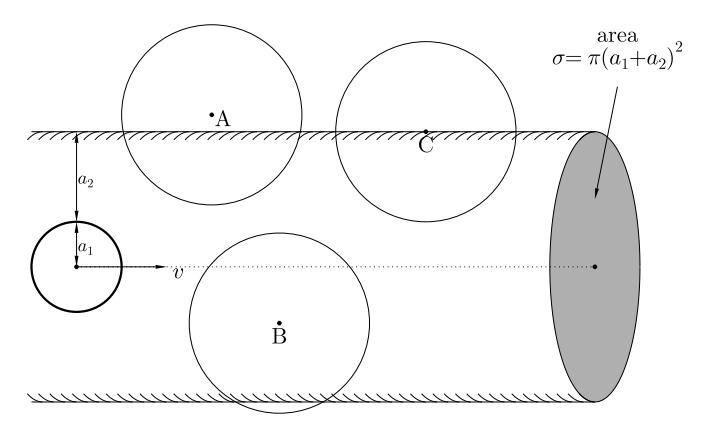
\includegraphics[width= 0.7\linewidth]{imagens/secaotransversal.png}
        \caption{Fonte: Concepts In Thermal Physics, Blundell and Blundell}
    \end{figure}

    Para o nitrogenio, \(\sigma_N = \pi(r_H + r_N)^2\) e para o oxigenio, \(\sigma_O = \pi (r_H + r_O)^2\). Como a atmosfera é feito de \(0,8 N\) e \(0,2 O\), é valido que 

    \[\sigma = 0,2\sigma_O + 0,8\sigma N\]

    Assim, temos 

    \[\boxed{\lambda = \frac{1}{\sqrt{2}n(0,8\sigma_0 + 0,2\sigma_0)}}\]

    \item Assumindo que a particula perde todo seu momento ao colidir com uma molécula de ar, temos \(\delta p = mv_{rms}\). Cada colisção acontece em um tempo \(\delta t =\tau\), assim, 
    \[F = \frac{\delta p }{\delta t} = \frac{mv_{rms}}{\tau} = n\sigma v_{rms}^2 \  \boxed{ = 3n\sigma k_BT}\]

    \item Utilizando a definição de pressão 
    
    \[P = \frac{F}{\sigma} = \ \boxed{3nk_B T} \]

    \item Utilizando a equação do equilíbrio hidrostático 
    
    \[\frac{dP}{dr} = -\rho g\]

    Como \(\rho\) e \(g\) são constantes, 

    \[P = -\rho g \int_h^0dh= \ \boxed{\rho g h}\]

    Onde \(h\) é a espessura da atmosfera.

    \item Igualando as pressões, 

    \[\rho g h = 3\frac{S_a}{S_w}nk_BT\]

    Resolvendo paar \(T\), temos 

    \[T = \frac{\rho g h}{3nk_B}\frac{S_w}{S_a}\]

    Como \(n\) é a densidade numérica de particulas e \(\rho\) é a densidade de massa, temos \(\rho/n = m\), assim

    \[\boxed{T= \frac{m g h}{3k_B}\frac{S_w}{S_a}}\]

    \item Fazendo uma média ponderada, 
    
    \[\boxed{m = 0,8 m_N + 0,2 m_O}\]

    \item a força que o eletron sente é dada por, 
    
    \[F = \frac{Ze^2}{4\pi \epsilon_0r^2}\]

    Igualando esta a força centrípeta

    \[\frac{Ze^2}{4\pi \epsilon_0r^2} = m_e \omega^2 r\]

    Porém, pela definição de momento angular, Temos

    \[L = m_er^2\omega \rightarrow \omega = \frac{L}{m_er^2} = \frac{n\hbar}{m_er^2}\]

    Substituindo na expressão anterior 

    \[\frac{Ze^2}{4\pi\epsilon_0 r^2} = m_e \left(\frac{n\hbar}{m_er^2}\right)^2 r\]

    Resolvendo para \(r\), 

    \[r = \frac{4\pi\epsilon_0 n^2\hbar ^2}{Z e^2 m_e}\]

    \item Para a água, temos, \(r_w = 2r_H + r_O\) e para o ar, \(r_a = 2(r_N + r_O)\), como \(S_i \propto r_i^2\), temos 
    
    \[\frac{S_w}{S_a} = \frac{(2r_H + r_O)^2}{4(r_N + r_O)^2}\]

    Assumindo que todos os elétrons estão no nível mais baixo (\(n=1\)), que \(Z_H = 1, \ Z_N = 7, \ Z_O = 8\) e que \(r\propto 1/Z\), temos 
    
    \[\boxed{\frac{S_w}{S_a}=\frac{(2/Z_H + 1/Z_O)^2}{4(1/Z_N + 1/Z_O)^2} \approx 15,73}\]

    \item Substituindo na fórmula, 

    \[T = \frac{(2\cdot 14 + 2 \cdot 16) \cdot 1,67 \cdot 10^{-27} \cdot 10^{5} \cdot 15,73}{3 \cdot 1,38\cdot 10^{-23}} \ \boxed{\approx 380\text{ K}}\]

    O que é uma estimativa bastante coerente com a relaidade, \(T = 373\) K.
\end{alternativas}
    



    
    
\end{pssolution*}
\end{pproblem}

\pts{3}
\begin{pproblem} (Adaptado Iran Problem Set)
    Dr. Shahram Abbassi é um dos cientistas iranianos mais reconhecidos no campo dos discos de acreção. Em uma de suas pesquisas recentes sobre a gigantesca nuvem molecular B32, ele descobriu uma estrela semelhante ao Sol no centro dessa nuvem específica. Segundo suas pesquisas, essa nuvem possui uma massa de $10^6 M_\odot$, um raio de $30 \, \text{pc}$ e uma viscosidade muito alta, tão grande que, se a nuvem entrasse em colapso, todo o sistema colapsaria com simetria esférica.

    O mais importante é calcular o calor específico a volume constante ($C_v$) para essa nuvem. Com base nos dados fornecidos e utilizando aproximações razoáveis, determine um limite para $C_v$ de modo que a acreção seja possível. Esses valores variam dependendo da massa e do raio da núvem? O que podemos concluir com o resultado?
\begin{pssolution*}{}{}
    Esse limite será dado pelo teorama do virial, quando, 

    \[\langle U \rangle = -2 \langle K \rangle\]

    Podemos modelar a nuvem como um gás, de modo que sua energia cinética seja dada por \(\frac{3}{2} N k_B T\). A sua energia potêncial é eneriga potencial de uma esfera, dada por \(U = -3GM^2/5R\). Assim

    \[\frac{3GM^2}{5R} = 3\frac{M}{m_p}k_B T\]

    Onde \(m\) é a massa de uma partícula da núvem.

    Desse modo, 

    \[T = \frac{GMm_p}{5k_B R}\]

    Em função do calor específico a volume consatnte, a energia é dada por, 

    \[M C_v T\]

    Voltando a igualdade, 

    \[C_v = \frac{3GM}{5R T}\]

    Substituindo \(T\), 

    \[\boxed{C_v = \frac{k_B }{m} \approx 4.1 \cdot 10^3 \text{ J kg\(^{-1}\) K\(^{-1}\)}}\]

    Note que esse valor depende apenas da massa das partículas que compões a núvem de gás. Para uma compostade hidrogênio, o valor é Surpreendentemente proximo do valor da água \(C_{v, agua} = 4,2\cdot 10^{3}\) J/kg K. 
\end{pssolution*}
\end{pproblem}



\newpage

\newpage

\section{Óptica e Telescópios}

\pts{3}
    \begin{pproblem} Um telescópio Kepleriano possuí duas lentes convergentes. A primeira possuí o raio de curavtura das duas faces igual a \(R = 2\text{ m}\) e a segunda possuí ambos os raios de curvatura igual a \(r = 0,5 \text{ m}\). Considerando que ambas as lentes possuem espessura desprezivel e são feitas de um material com indíce de refração \(n=1,4\). Calcule o diâmetro e o aumento do telescópio sabendo que este telescópio é um f/12.
    \end{pproblem}

\pts{5}
    \begin{pproblem}
        Nessa questão, vamos nos familiarizar com uma das ferramentas mais poderosas da óptica, a \textit{óptica geométrica}. O objetivo dessa ferramenta é modelar lentes e espelho em forma de matrizes. Isso é muito útil para resolver questões envolvendo associações de diversas lentes e é um método de resolver problemas de óptica geométrica (praticamente) sem usar geometrica. Mas para isso, se atente as seguintes definições na imagem a seguir

        \begin{figure}[H]
            \centering
            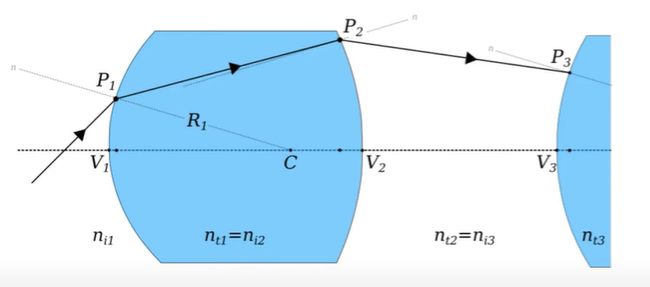
\includegraphics[width=0.9\linewidth]{imagens/lentes1.png}
            \caption{Esquema 1}
        \end{figure}

        Todas as linhas pontilhadas são paralelas ao eixo óptico, representado pela seta horizontal. É denotado por \(P_k\) o ponto onde a luz passa de um meio para o outro, \(y_k\) a coordenda vertical do ponto \(P_k\). São utilizados os subscritos \(i\) e \(t\) para se referir a incidente e transmitido, reespectivamente, então, por exemplo, \(\alpha_{i,k}\) é o ângulo que o raio de incidente luz faz com a horizontal no ponto \(P_k\), já o ângulo \(\alpha_k\) é o ângulo entre a horizontal e o centro da lente \(k\).
        

        Para essa questão, vamos considerar que todos os ângulos de interesse são pequenos, de modo que \(\tan\theta \approx \sin\theta \approx \theta\).
        \begin{alternativas}
            \item Partindo da Lei de Snell, encontre uma relação entre \(n_{i,1}\), \(n_{t,1}\), \(\alpha_1\), \(\alpha_{i,1}\) e \(\alpha_{t,1}\).
        
        É facil perceber que \(\alpha_k = y_k/R_k\). Utilizando-se desse fato

            \item Encontre uma relação para \((1) \ n_{t,1}\alpha_{t,1}\) e \((2) \ y_{t,1}\). Deixe suas respostas em função de \(n_{i,1}\), \(\alpha_{i,1}\), \(y_{i,1}\) e \(\mathcal{D}_1\), para
            \[\mathcal{D}_1 = \frac{n_{t,1}-n_{i,1}}{R_1}\]

        Agora vamos para mais uma definição, seja o vetor \(\mathbf{r}_{t,1}= (n_{t,1}\alpha_{t,1}, \ y_{t,1})\) e \(\mathbf{r}_{i,1}= (n_{i,1}\alpha_{i,1}, \ y_{i,1})\).
        
            \item É possível escrever as duas equações que encontramos no item anterior na forma matricial, de forma:
            \[\mathbf{r}_{t,1}=\mathcal{R}_1\mathbf{r}_{i,1}\]
            Encontre a matriz \(2\times 2\) equivalente à \(\mathcal{R}_1\).

        Nosso interesse agora é encontrar as relações entre os pontos \(P_2\) e \(P_1\).

            \item Encontre uma equação para \(n_1\alpha_{i,2}\) e \(y_{i,2}\). Utilizando o raciocínio do item anterior, deixe sua resposta na forma
            \[\mathbf{r}_{i,2}=\Gamma_{2,1}\mathbf{r}_{t,1}\]
            Onde \(\Gamma_{2,1}\) também é uma matriz \(2\times 2\).

            \item Definimos a matriz da lente, \(\mathcal{A}_{2,1}\) da seguinte equação:
            \[\mathbf{r}_{i,2} = \mathcal{A}_{2,1}\mathbf{r}_{i,1}\]
            De modo que

            \[\mathcal{A}_{2,1} = \begin{pmatrix}
                a_{11} & a_{12} \\
                a_{21} & a_{22} \\
            \end{pmatrix}\]

            Encontre explicitamente \(\mathcal{A}_{2,1}\).

            \item Dentre todas as propriedades da matriz da lente, a mais curiosa delas é que o termo \(a_{12}\) equivale a \(-1/f\) onde \(f\) é o foco da lente. Prove esse resultado. (Dica: você consiguira escrever \(-a_{12}\) com uma equação bem conhecida da óptica).
        
        Agora, vamos colocar a mão na massa e fazer utilizações praticas da óptica matricial.

            \item Refaça o exercício anterior utilizando óptica matricial.
        
            \item Considere o seguinte esquema:
                \begin{figure}[H]
                    \centering
                    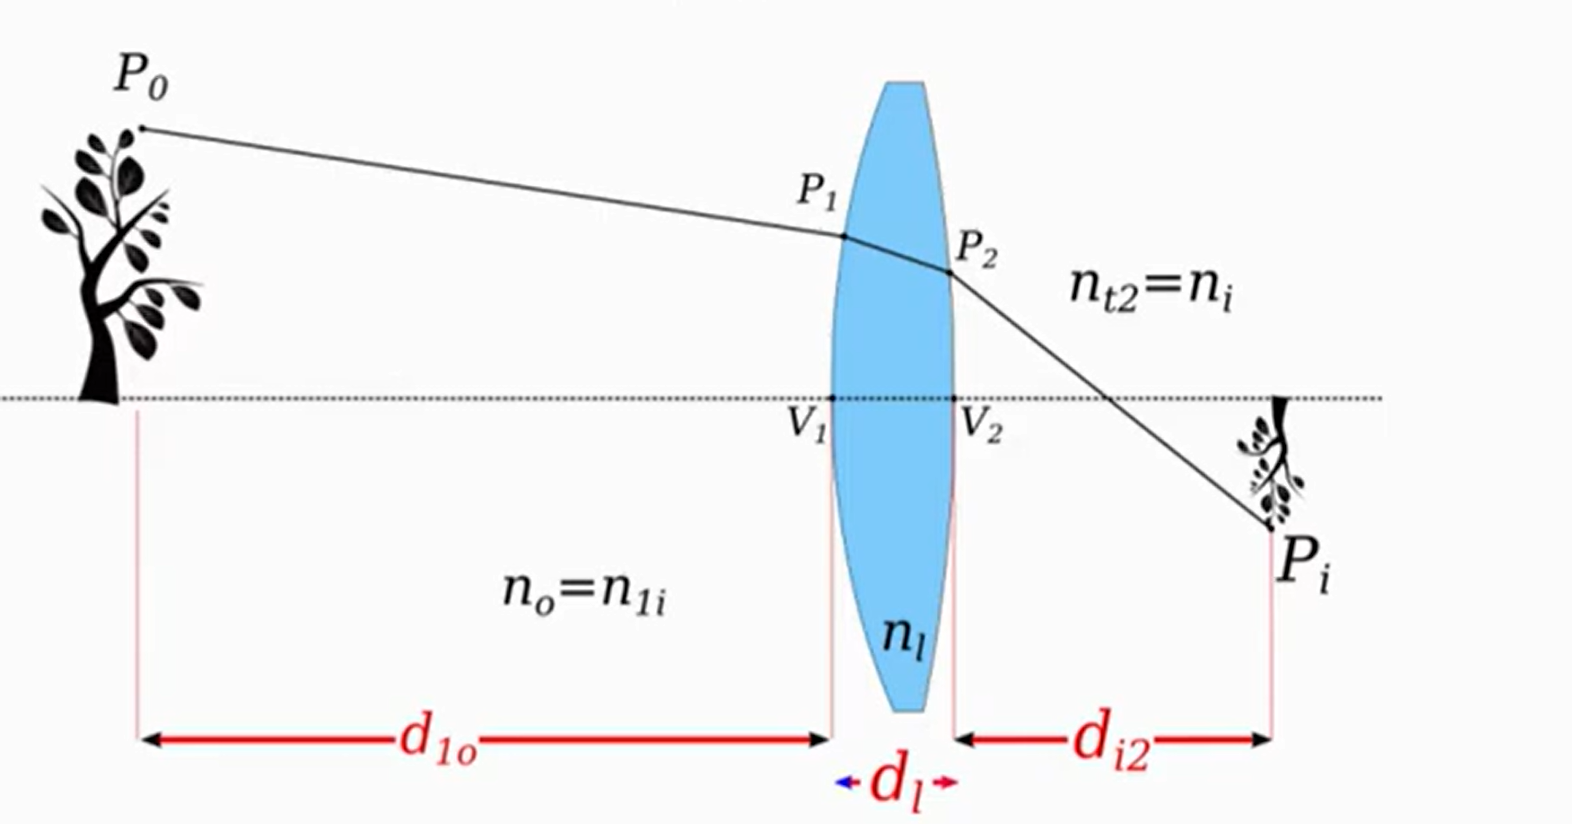
\includegraphics[width=0.9\linewidth]{imagens/lentes2.png}
                    \caption{Esquema 2}
                \end{figure}
                 Ecnontre \(y_i\) em função de \(y_0\) e dos dados na imagem.
                 
            \item Se a lente estiver entre dois meios diferentes, \(n_{i,1} \ne n_{t,2}\) temos a seguinte relação:
            \[a_{12} = -\frac{n_{i,1}}{f_0}=-\frac{n_{t,2}}{f_I}\]
                Utilizando-se disse, refaça a questão anterior, considerando que entre as duas lentes á água de \(n_w = 4/3\).
        
            \item Um arranjo muito comum de lentes é a Objetiva de Tessar, presente em muitas cameras pela sua eficiencia em diminuir efeitos de aberração e astigmatismo. O Arranjo tem a seguinte forma:
                \begin{figure}[H]
                    \centering
                    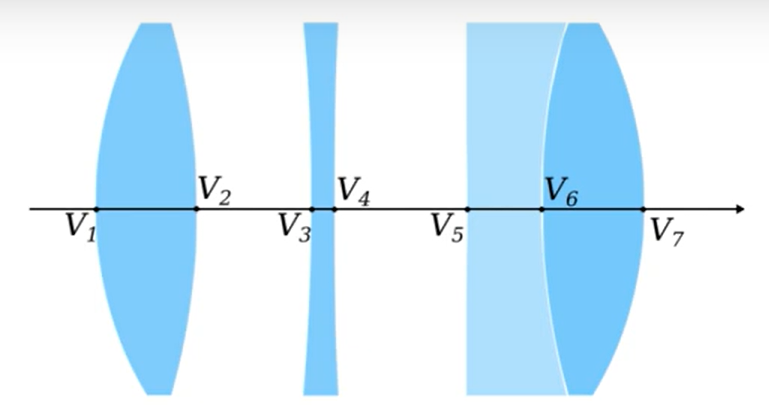
\includegraphics[width=0.7\linewidth]{imagens/lentes3.png}
                    \caption{Esquema Objetiva Tessar}
                \end{figure}
                Encontre a Matrix da Lente equivalente, \(\mathcal{A}_{1,7}\) em função de \(\mathcal{R}_i\) e \(\Gamma_{i,j}\).
        \end{alternativas}
    \begin{pssolution*}{}{}
        \begin{alternativas}
            \item A lei de Snell nos diz que \(n_{i,1}\theta_{i,1} = n_{t,1}\theta_{t,1}\). Onde \(\theta\) são os ângulso que a luz faz com a normal. Note que podemos escrever ambos os ângulos \(\theta\) como:
            \[\theta_{i,1} = \alpha_1 + \alpha_{i,1}, \ \ \theta _{t,1} = \alpha_1 + \alpha_{t,1}\]

            Logo, a relação que procuramos é 

            \[\boxed{n_{i,1}(\alpha_1+\alpha_{i,1}) = n_{t,1}(\alpha_1+\alpha_{t,1})}\]

            \item Substituindo \(\alpha_1 = y_1/R_1\), temos
            
            \[n_{i,1}(y_1/R_1+\alpha_{i,1})=n_{t,1}(y_1/R_1 +\alpha_{t,1})\]

            isolando \(n_{t,1}\alpha_{t,1}\)

            \[n_{t,1}\alpha_{t,1} = n_{i,1}\alpha_{i,1}+ \frac{y_1}{R_1}(n_{i,1}-n_{t,1})\]

            Em termos de \(\mathcal{D}_1\) 

            \[n_{t,1}\alpha_{t,1} = n_{i,1}\alpha_{i,1} - y_1\mathcal{D}_1\]

            Note que \(y\) não moda imediatamente após a transmissão da luz. Logo \(y_1\equiv y_{i,1}\equiv y_{t,1}\).

            \item Na forma matricial
            
            \[\left(\begin{matrix}
                n_{t,1}\alpha_{t,1} \\
                y_{t,1}\\
            \end{matrix}\right) = \left(\begin{matrix}
                1 & - \mathcal{D}_1 \\
                0 & 1
            \end{matrix}\right)\left(\begin{matrix}
                n_{i,1}\alpha_{i,1} \\
                y_{i,1}\\
            \end{matrix}\right)\]

            Assim, nossa matriz \(\mathcal{R}_1\), também conhecida como matriz refração é dada por:

            \[\boxed{\mathcal{R}_1 = \left(\begin{matrix}
            1 & -\mathcal{D}_1 \\
            0 & 1 \\
            \end{matrix}\right)}\]

        \item Primeiro, vamos achar a altura do ponto \(2\). Seja \(d_{21}\) a espessura da lente. Utilizando trigonometria obtemso
        
        \[y_{i,2} = y_{t,1} + \alpha_{t,1}d_{21}\]

        Temos que \(\alpha_{t,1}\) e \(\alpha_{i,2}\) são alternos internos. Ou seja \(\alpha_{t,1}=\alpha({i,2}\). Como o indice de refração dentro da lente é constante, temos
        \[\] 
        \end{alternativas}
\end{pssolution*}

\end{pproblem}

\pts{2}
\begin{pproblem}
    A teoria ondulatória da luz demonstra que um foco perfeito não é possível devido aos efeitos de difração associados à abertura finita da lente. Essa falta de foco perfeito impede que objetos muito próximos sejam distinguidos. Este problema pode ser estudado de dois pontos de vista diferentes:

    A teoria ondulatória da luz prevê que uma lente de diâmetro $D$ não pode focar um feixe paralelo de luz com comprimento de onda $\lambda$ em um ângulo menor que o limite de difração:
    \begin{equation}
        \theta_m \approx 1.22 \frac{\lambda}{D}
    \end{equation}

    Considere agora uma abordagem quântica, os fótons que são focados pela lente. Esses fótons são conhecidos por terem passado em algum lugar dentro de um raio do centro da lente. A incerteza na posição $x$ está associada a uma incerteza no componente $x$ do momento do fóton. Consequentemente, um fóton que, na ausência dessa incerteza, teria sido trazido para o eixo óptico do plano focal, pode agora ser desviado por um ângulo $\theta \ll 1$.

    Considere o comprimento de onda de de Broglie $\lambda = \frac{h}{p}$. Encontre um limite para $\theta$.

    \textbf{DICA:} o princípio de incerteza de Heisenberg, relaciona a impressição entre as medidas de momento e posição de uma particula por 
    \[\Delta p_x \Delta x = \frac{\hbar}{2}\]

\begin{pssolution*}{}{}
    O momento de um fóton é dado por \(p = h/\lambda\) e sabemos que o foton possui \(\Delta x = D\) utilizando o princípio da incerteza de Heisenberg

    \[\Delta p_x = \frac{\hbar}{2D}\]

    Utilizando que \(\theta \approx \frac{\Delta p_x}{p}\), obtemos
    \[\boxed{\theta \approx\frac{\lambda\hbar}{2D h} = \frac{1}{4\pi}\frac{\lambda}{D}}\]
\end{pssolution*}
\end{pproblem}

\pts{3}
\begin{pproblem} (Apostila Magna)
    Prove que a quantia \(n_iR_i\sin \theta_i\) para cascas esféricas adjacentes entre si, em que \(n_i\) é o índice de refração da i-ésima casca esférica, \(\theta_i\) é o ângulo que o raio de luz faz com a normal da i-ésima casca esférica e \(R_i\) é o raio da i-ésima casca esférica, é uma invariante
    
\end{pproblem}

\pts{4}
\begin{pproblem}
    O indídice de refração da atmosfera de um planeta é dado por, 

    \[n(h) = \frac{n_0}{1+\epsilon h}\]

    Onde \(n_0\) e \(epsilon\) são constantes.

    \begin{alternativas}
        \item Um raio de luz atinge a atmosfera paralelamente a superfície, há uma altura \(h'\ll R\), como será a trajetória?
        \item Sabendo a trajetória do raio de luz, calcule o Raio do planeta.
    
        \textbf{Dica:} Você pode achar útil a seguinte relação, 

        \[\int \frac{t}{\sqrt{a-bt^2}}dt = -\frac{1}{b}\sqrt{a-bt^2}+C\]
    \end{alternativas}
\begin{pssolution*}{}{}
    \begin{alternativas}
        \item Defidindo \(ds = \sqrt{dx^2+dh^2}\) como sendo o elemnto infinitesimal de arco, temos, 
        \[\sin\theta = \frac{dx}{ds}, \ \ \cos\theta = \frac{dh}{ds}\]

        Como o meio é contínuo, podemos escrever, 

        \[n(h)\sin\theta(h)=cte\]

        Assim, 

        \[n\frac{dx}{ds} = K\]

        Substituindo \(n\), 

        \[\frac{dx}{ds} = \frac{K(1+\epsilon h)}{n_0}\]

        Porém, pela definição de \(s\), temos, 

        \[\left(\frac{dx}{ds}\right)^2 + \left(\frac{dh}{ds}\right)^2 = 1\]

        Substituindo \(dx/ds\), 

        \[\frac{dh}{ds} = \sqrt{1- \left(\frac{K(1+\epsilon h)}{n_0}\right)^2}\]

        Usando uma regra da cadeia, 

        \[\frac{dh}{dx} = \frac{dh/ds}{dx/ds} = \frac{\sqrt{1- \left(\frac{K(1+\epsilon h)}{n_0}\right)^2}}{\frac{K(1+\epsilon h)}{n_0}}\]

        Simplficando a expressão, 

        \[\frac{dh}{dx} = \frac{\sqrt{n_0^2 - K^2(1+\epsilon h)^2}}{K(1+\epsilon h)}\]

        Para resolver essa E.D.O, vamos criar a variável \(u = 1+\epsilon h\), de modo que, 

        \[dh = \frac{du}{\epsilon}\]

        Assim, 

        \[\frac{du}{dx} = \epsilon\frac{\sqrt{n_0^2 - K^2u^2}}{Ku}\]

        Separando os termos e integrando, 

        \[\int \frac{u}{\sqrt{n_0^2 - K^2u^2}} du = \frac{\epsilon}{K}\int dx\]
    
        A integral do lado esquerdo, é a mesma fornecida pela questão, assim, 

        \[-\frac{1}{K^2}\sqrt{n_0^2-K^2u^2} = \frac{\epsilon}{K}x + C\]

        Trabalhando nessa expressão, 

        \[\sqrt{n_0^2-K^2u^2} = -\epsilon K x - K^2C\]

        \[n_0^2-K^2u^2 = (\epsilon K x + K^2C)^2\]

        Substituindo \(u\), 

        \[n_0^2-K^2(1+\epsilon h)^2 = \epsilon^2K^2x^2 + 2\epsilon K^3 C x + K^4C^2\]

        Rearranjando os termos, 

        \[\epsilon^2K^2x^2 + 2\epsilon K^3 C x + K^2(1+\epsilon h)^2 = n_0^2 - K^4C^2 \]

        \[\epsilon^2x^2 + 2\epsilon K C x + (1+\epsilon h)^2 = n_0^2/K^2 - K^2C^2 \]

        Dividindo por \(\epsilon^2\), 

        \[x^2 + \frac{2KC}{\epsilon}x + \frac{K^2C^2}{\epsilon^2} + \left(h+\frac{1}{\epsilon}\right)^2 = \left(\frac{n_0}{\epsilon K}\right)^2\]

        Juntando o produto notável, 

        \[\boxed{\left(x + \frac{KC}{\epsilon}\right)^2+\left(h+\frac{1}{\epsilon}\right)^2 = \left(\frac{n_0}{\epsilon K}\right)^2}\]
   
        Que é justamente a equação de um círculo de raio \(\frac{n_0}{\epsilon K}\) e centro \(C = (-\frac{KC}{\epsilon}, \ - \frac{1}{\epsilon})\).

        \item No caso de um raio que tangência o planeta, temos que o mesmo possuí \(\theta_0 = \pi/2\) e \(h_0=0\). Assim, utilizando, 
        
        \[n(h)\sin\theta(h) = n_0\sin\theta_0 = K\]

        Obtemos \(K = n_0\), assim, o raio do planeta é dado pelo raio da trajetória (O raio de luz é tangênte a superfície) e, portanto, 

        \[\boxed{R = \frac{1}{\epsilon}}\]
    \end{alternativas}
    
\end{pssolution*}
\end{pproblem}

\newpage

\section{Cosmologia}

\pts{5}
\begin{pproblem}
    A Equação de Friedmann é uma das mais importantes para o estudo da cosmologia e do estudo sobre o universo. O objetivo do problema é deduzir as equações fundamentais da cosmologia. Primeiro, vamos com algumas definições:
    \begin{enumerate}[label=\roman*)]
        \item Devido a expansão do Universo, a distância entre dois pontos é dada por:
        \[r(t) = r_0 a(t)\]
        Onde \(a(t)\) é conhecido como o fator de escala e \(r_0\) é a distância medida em \(t=0\). 
        
        \item O Universo segue a métrica de Robertson-Walker, a mesma pode ser simplificada para:
        \[-c^2dt^2 + dr^2=0\]
        \begin{alternativas}
            \item Encontre uma expressão para a distância comóvel, \(r_0\), na forma de integral, a partir das definições dadas anteriormente.
            \\
            \item A Primeira Equação de Friedmann tem forma:
            \[H(t)^2 \equiv \left(\frac{\dot{a}}{a}\right)^2 = k_1\varepsilon(t) + \frac{C}{r_0^2a^2}\]
            Encontre os valores das constanets \(k_1\) para um universo esférico, em função de constantes fundamentais. Na equação acima, \(\varepsilon(t)\) é a densidade de energia do universo, \(C\) é uma constante relacionada a sua energia e \(a\) é o fator de escala.

            \textbf{Dica: }Você pode obter essa equação tanto por conservação de energia ou utilizando a segunda lei de Newton.

            \item Repita o item anterior para um universo cilíndrico se expandindo radialmetne.
            A equação encontrada deve ter forma, 

            \[\left(\frac{\dot{a}}{a}\right)^2 = f(a)\varepsilon(t) + \frac{C'}{r_0^2a^2}\]

            Encontre a função \(f(a)\).

            \item Voltando agora para um "universo normal". Em cosmologia, definimos a densidade crítica de energia, como sendo a densidade de energia de um universo em que \(C = 0\). Encontre uma expressão para a densidade crítica.
            \item Re-escreva a primeira equação de Friedmann em função de:
            \[\Omega(t) = \frac{\varepsilon(t)}{\varepsilon_c(t)}\]
            Onde \(\varepsilon_c(t)\) é a densidade crítica de energia.
        \end{alternativas}
    \end{enumerate}
\begin{pssolution*}{}{}
    \begin{alternativas}
        \item Isulando \(d_r\), 
        \[d_r = cdt\]

        Mas por definição, \(r(t) = r_0a(t) \rightarrow d_r = r_0da\). Substituindo, 

        \[dr_0 = c\frac{dt}{a(t)}\]

        Integrando dos dois lados, 

        \[r_0 = c\int\frac{dt}{a(t)}\]

        \item \textbf{Método 1: Conservação de energia}
        Considere uma particula de massa \(m\) localizada em um ponto do universo. A sua energia em relação ao centro do universo é dada por, 

        \[E = \frac{mv^2}{2} - \frac{GM(r)m}{r}\]

        Onde \(v = \dot{r} = r_0\dot{a}\) e \(M(r) = \frac{4}{3}\pi r^3\rho(t)\).  Dividindo a equação por \(m/2\) e aplicando as substituições, temos, 

        \[\frac{2E}{m} = r_0^2\dot{a}^2 - \frac{G}{r_0a}\frac{8\pi (r_0a)^3\rho(t)}{3}\]

        Simplificando, 

        \[\frac{2E}{m} = r_0^2\dot{a}^2 - \frac{8\pi G r_0^2a^2\rho(t)}{3}\]

        Multiplicando ambos os lados por \(\frac{1}{r_0^2a^2}\), obtemos, 

        \[\frac{2E}{mr_0^2a^2} = \left(\frac{\dot{a}}{a}\right)^2 - \frac{8\pi G\rho(t)}{3}\]

        Reorganiznaod a equação e ultilizando a equivalencia massa energia, \(m = E/c^2 \rightarrow \rho(t) = \varepsilon(t)/c^2\), temos, 

        \[\left(\frac{\dot{a}}{a}\right)^2 = \frac{8\pi G}{3 c^2}\varepsilon(t) + \frac{2E}{mr_0^2a^2}\]

        Da onde podemos concluir que, 

        \[\boxed{k_1 = \frac{8\pi G}{3c^2}}\]


        \textbf{Método 2: Segunda Lei de Newton}

        Escrevendo a segunda lei de newton para um corpo com relação ao centro do unvierso, 

        \[-\frac{GM(r)m}{r^2} = m\frac{d^2r}{dt^2}\]

        Note que, ao se expandir, o universo não cria massa, então a massa contida em uma camada \(r\), será constante ao longo do tempo, usando dessa propriedade, temos que, 

        \[\frac{d^2r}{dt^2} = -\frac{GM(r)}{r^2}\]

        Multiplicando ambos os lados por \(dr/dt\), 

        \[\frac{dr}{dt}\frac{d^2r}{dt^2} = -\frac{GM(r)}{r^2}\frac{dr}{dt}\]

        Reescrevendo, 

        \[\dot{r}\frac{d\dot{r}}{dt} = -\frac{GM(r)}{r^2}\frac{dr}{dt}\]

        Multiplicando ambos os lados por \(dt\), 

        \[\dot{r}d\dot{r} = -GM(r)\frac{dr}{r^2}\]

        Substituindo \(r = r_0a\), 

        \[r_0^2\dot{a}d\dot{a} = -\frac{GM(r)}{r_0} \frac{da}{a^2}\]

        Integrando dos dois lados, 

        \[r_0^2\int\dot{a}da = -\frac{GM(r)}{r_0^2} \int\frac{da}{a^2}\]

        \[\frac{r_0^2\dot{a}^2}{2} = \frac{GM(r)}{r_0 a} + A\]

        Onde \(A\) é uma constante de integração. Substituindo \(M(r)\), 

        \[\frac{r_0^2\dot{a}^2}{2} = \frac{4\pi G r_0^2 a^2}{3c^2}\varepsilon(t) + A\]

        Multiplicando a expressão por \(2/a^2r_0^2\), temos, 

        \[\left(\frac{\dot{a}}{a}\right)^2 = \frac{8\pi G}{3c^2} \varepsilon(t) + \frac{2A}{r_0^2a^2}\]
    
        De onde podemos concluir, igualmente, que, 

        \[\boxed{k_1 = \frac{8\pi G}{3c^2}}\]

        \item Utilizando a lei de gauss, 
        
        \[\oint\mathbf{g}\cdot d\mathbf{S} = -4\pi G M(r)\]

        Onde, 

        \[\oint \mathbf{g} \cdot d\mathbf{S} = -g(2\pi r L)\]

        Para uma simetria cilíndrica. Substituindo na equação, 

        \[g = \frac{4\pi G M(r)}{2\pi r L} = \frac{2G M(r)}{r L}\]

        Utiliznado o método da conservação de energia, temos primeiramente temos que calcular a energia potencial, 

        \[U = -\int F dr = -\int \frac{2GM(r)m}{rL}dr = -\int\frac{2GM(r)m}{L}\frac{da}{a} -\frac{2GM(r)m}{L}\ln(a)\]

        Por conservação de energia, 

        \[E = \frac{m r_0^2\dot{a}^2}{2} - \frac{2GM(r)m}{L}\ln(a)\]

        Substituindo \(M(r) = \pi r_0^2a^2 L \varepsilon(t)/c^2\), 

        \[E = \frac{m r_0^2 \dot{a}^2}{2} - \frac{2\pi r_0^2a^2G m \ln (a)}{c^2}\varepsilon(t)\]

        Reorganizando, 

        \[\left(\frac{\dot{a}}{a}\right)^2 = \frac{4\pi G \ln(a)}{c^2}\varepsilon(t) + \frac{2E}{mr_0^2a^2}\]

        Da onde podemos obter, 

        \[\boxed{f(a) = \frac{4\pi G}{c^2}\ln(a)}\]

        \item A equação de Friedmann para \(C=0\) se reduz a
        
        \[H(t)^2 = \frac{8\pi G}{3c^2}\varepsilon_c(t)\]

        Isolando \(\varepsilon_c(t)\), 

        \[\boxed{\varepsilon_c(t) = \frac{3c^2}{8\pi G}H^2(t)}\]

        Pela definição, 

        \[\varepsilon(t) = \Omega (t) \varepsilon_c(t)\]

        Substituindo na equação, 

        \[H^2(t) = \frac{8\pi G}{3c^2}\Omega(t)\varepsilon_c(t) + \frac{C}{r_0^2a^2}\]

        Substituindo \(\varepsilon_c(t)\), 

        \[H^2(t) = H^2(t)\Omega(t) + \frac{C}{r_0^2a^2}\]

        Resolvenod para \(H^2(t)\), 

        \[\boxed{H^2(t) = \frac{C}{r_0^2a^2(1-\Omega(t))}}\]
    \end{alternativas}
    
\end{pssolution*}
\end{pproblem}

\pts{3}
\begin{pproblem}(Adaptado NAO 2019) Considere um universo plano em que a consante gravitacional deixa de ser constante e passa a ser definida por
    \[G(a) = G_0 f(a)\]
    Onde \(f(a)\) é uma função do fator de escala.
    \begin{alternativas}
        \item Como se daria a Equação de Friedmann nesse universo? Assuma que o universo é plano, \(C = 0\) e que ele é composto apenas por matéria bariônica ("clara"). Deixa sua resposta em função de \(H_0\), \(f(a)\), \(a\) e \(\Omega_{m,0}\), onde \(H_0\) é o valor da constante de Hubble no tempo atual, e \(\Omega_{m,0}\) é o parâmetro de densidade,
        
        No caso em que \(f(a) = e^{b(a-1)}\), onde \(b=2\).
        
        \item Estime a idade desse universo assumindo que ele é constituído apenas de máteria bariônica (matéria "clara").
                
        \item Qual o comportamento da idade quando \(t\rightarrow \infty\)?
    \end{alternativas}

    Talvez você ache as seguintes relações úteis:
    \begin{paracol}{2}
        \[\int_0^\infty x^2e^{-x^2} = \frac{\sqrt{\pi}}{4}\]

        \switchcolumn

        \[\int_0^1 x^2e^{-x^2} \approx 0,189\]
    \end{paracol}
\begin{pssolution*}{}{}
    \begin{alternativas}
        \item Para um universo plano e contendo apenas matéria a equação de Friedmann tem cara, 
        \[H(t)^2 = H_0^2\Omega_m\]

        Onde \(\Omega_m = \frac{\rho_m(t)}{\rho_{c, 0}}\) onde 

        \[\rho_c = \frac{3 H_0^2}{8\pi G}\]

        Para matéria bariônica, 

        \[\rho_m(t) = \rho_0a(t)^{-3}\]

        Então, 

        \[\Omega_m = \Omega_{m,0} f(a)a^{-3}\]

        Para um universo só de matéria bariônica, \(\Omega_{m,0} = 1\),
        
        Assim, 

        \[\boxed{H(a)^2 = H_0^2 \Omega_{m,0} f(a)a^{-3} \equiv H_0^2 f(a)a^{-3}}\]

        \item Usando que \(H = (\dot{a}/a)\), temos, 
        
        \[t = \int dt = \int da\frac{dt}{da} = \int \frac{da}{\dot{a}} \]

        Multiplicando por \(a/a\), 

        \[t = \int\frac{a}{\dot{a}a}da = \int \frac{da}{H(a)a}\]

        Substituindo o valor de \(H(a)\) encontrado no item anterior, 

        \[t = \frac{1}{H_0^2}\int\frac{da}{\sqrt{f(a)a^{-3}}} = \frac{1}{H_0^2}\int a^{3/2} e^{-b(a-1)/2}da = \frac{e^{b/2}}{H_0^2}\int a^{3/2}e^{-ba/2}da\]
        
        Usando uma substituição da forma \(x = \sqrt{ba/2}\), temos, 

        \[t = \frac{4\sqrt{2}e^{b/2}}{b^{3/2}H_0}\int x^2e^{-x^2}\]

        Os limites de integração vão de \(a=0\) (inicio do universo) até \(a=1\) (momento atual), como fizemos a substituição em x, 

        \[x = \sqrt{\frac{ab}{2}}\]

        \[t = \frac{4\sqrt{2}e^{b/2}}{b^{3/2}H_0}\int_0^{\sqrt{b/2}} x^2e^{-x^2}\]

        Substituindo \(b=2\), 

        \[t = \frac{4\sqrt{2}e}{2^{3/2}H_0}\int_0^{1} x^2e^{-x^2}\]

        Substituindo os valores e ultilizando a integral fornecida, obtemos, 

        \[\boxed{t \approx 15 \text{Gyr}}\]

        O que é proximo do nosso universo!!

        \item Mudando os limites da integral para um tempo infinito, \(a(t)\rightarrow \infty\), 
        
        \[\boxed{t_\infty = \frac{4\sqrt{2}e}{2^{3/2}H_0}\int_0^{\infty} x^2e^{-x^2} = \frac{\sqrt{2\pi}e}{2^{3/2}H_0} \approx 34.1\text{ Gyr}}\]

    \end{alternativas}
    
\end{pssolution*}
\end{pproblem}

\pts{5}
\begin{pproblem}(Lista 8 - 2021)
    A equação de Friedmann é:
\begin{equation}
    H^2 = \left( \frac{\dot{a}}{a} \right)^2 = \frac{8\pi G \varepsilon}{3c^2} - \frac{k c^2}{a^2},
\end{equation}

em que $a$ é o fator de escala no tempo $t$, $\varepsilon$ é a densidade de energia no tempo $t$ e $k$ é o parâmetro que informa a geometria do universo, podendo assumir qualquer valor real. Considerando um universo composto apenas de matéria bariônica não relativística e resolvendo essa equação diferencial não linear para $k > 0$, obtêm-se as seguintes soluções em termos do parâmetro $\theta \in [0, 2\pi]$:

\begin{align}
    a(\theta) &= \frac{4\pi G \varepsilon_0}{3k c^4} \left( 1 - \cos\theta \right), \\
    t(\theta) &= \frac{4\pi G \varepsilon_0}{3k^{3/2}c^5} \left( \theta - \sin\theta \right).
\end{align}

Seja um universo com $\Omega_0 = 4$ e $H_0 = 67,4 \ \text{km/s/Mpc}$.

\begin{alternativas}
    \item A partir da equação de Friedmann, mostre que $k c^2 = H^2 \left( 1 - \Omega \right) a^2$. Por fim, reescreva as equações paramétricas de $a$ e $t$ em termos do parâmetro de densidade atual $\Omega_0$ e da constante de Hubble atual $H_0$, além do parâmetro $\theta$. Não substitua os seus respectivos valores numéricos.
    \item Encontre a idade $t_0$ do universo em questão em termos de $H_0$ e em seguida em bilhões de anos.
    \item O chamado \textit{Lookback time}, $\Delta t_L$, representa quanto tempo no passado o universo estava com certo fator de escala $a$. Qual é $\Delta t_L$ em bilhões de anos para quando o tamanho do universo era $1/3$ do que é atualmente?
    \item Determine $\theta_n$ e em seguida $t_n$ para os quais $H = 0$.
\end{alternativas}
\begin{pssolution*}{}{}
    \begin{alternativas}
        \item 
    \end{alternativas}
    
\end{pssolution*}
\end{pproblem}

\pts{5} 
\begin{pproblem}(Lista 6 - 2022)
aaa
\end{pproblem}

\newpage

\section{Miscelânia}
\pts{4}
\begin{pproblem} \clock{1}{0}
    Dudu Leiteiro, estava observando o céu, no interior de sua fazenda no Mato Grosso do Sul e observou o sistema binário formado pelas estremas Iaum e Sezenem. Dudu, oberservou as estrelas e coletou os seguintes dados, com um intervalo de 6 meses entre eles:
    \\
    \begin{center}
        \begin{tabular}{|c|c|c|}
            \hline % Linha horizontal superior
            Medida & Iaum & Sezenem   \\ 
            \hline
            Ascenção Reta \(1\) & \(4^h19^m53,91^s\) & \(4^h19^m53,078^s\) \\
            Ascenção Reta \(2\) & \(4^h19^m53,92^s\) & \(4^h19^m53,077^s\) \\
            Declinação \(1\) & -\(13^\circ \ 33' \ 45,28''\) & -\(13^\circ \ 33' \ 47,78''\) \\
            Declinação \(2\) & -\(13^\circ \ 33' \ 45,20''\) & -\(13^\circ \ 33' \ 48,03''\) \\
            \hline
        \end{tabular} 
\end{center}
    Com esses dados, você e Dudu Leiteiro, juntos vão analizar propriedades desse sistema binário. O primeiro passo importante para isso, é encontrar as coordenadas do centro de massa do sistema, denotadas pelo subscrito \(_{CM}\). Você lembra que em uma das aulas sobre o estudo de binárias, seu professor, LuCav, te ensinsou que:
    \[
    \delta_{CM} = \delta_A + \Delta\delta_A
    \]

    \[
    \alpha_{CM} = \alpha_A + \Delta\alpha_A
    \]

    Onde \(\delta_A\) e \(\alpha_A\) são as coordenadas de uma das estrelas do binário e \(\Delta\) representa a diferença de coordenadas entre a estrela e o centro de massa, temos a seguinte relação:

    \[
    \frac{a_A}{a} = \frac{\Delta\delta_A}{\Delta\delta_{CM}} = \frac{\Delta\alpha_A}{\Delta\alpha_{CM}}
    \]

    Onde \(a_A\) é a distância da estrela \(A\) até o \(CM\), \(a\) o semi-eixo maior da órbita e \(\Delta x_{CM}\) a variação das coordenadas do \(CM\). 
    
    \textbf{a)} Sabendo que Iaum possuí \(3/2\) da massa de Sezenem, calcule \(\Delta\delta_{CM}\) e \(\Delta\alpha_{CM}\).
    
    \textbf{b)} Com isso e considerando que as variação angulares são pequenas o suficiente para triângulos esféricos serem planos, encontre a paralaxe do sistema e sua distância até a Terra.

    \textbf{c)} Considerando a massa de Iaum, \(M_I = 4,9 M_\odot\), e o período do sistema igual a \(P = 29,01\) anos, calcule o maior redshift advindo de Sezenem, sendo que ambas as órbitas são circulares e Sezenem possuí velocidade tangencial de \(\mu = 1509''/ano\).

\end{pproblem}

\pts{3}
\begin{pproblem} Marisso estava cansado de não conseguir encontrar com precisão a posição de uma estrela em seu telescópio e decidiu investigar os efeitos que poderiam estar causando essse erro aparente. Após ler alguns artigos, ele descobriu \(2\) principais efeitos que fazem um objeto aparentar estar em um ângulo \(\Delta \theta_i\), desviado da sua posição original, são eles: \textit{Paralaxe} e \textit{Aberração Estelar}. Nessa questão, seu objetivo é ajudar Marrisso, a entender o porque desses efeitos acontecerem.
    \begin{alternativas}
        \item A paralaxe é o mais básico deles e ocorre por causa da mudança de posição da Terra ao longo do Ano. Considere que uma estrela está localizada de tal modo que a linha \(Sol-Estrela\) é perpendicular ao plano da órbota da Terra. Desenhe o esquema da situação e, considerando o raio da órbita da Terra como \(r\) e a distância da estrela como \(d\), obtenha uma fórmula para \(\Delta \theta_p\) causado pela paralaxa.
        
        \item Suponha agora, que a linha \(Sol-Estrela\) faça um ângulo \(\phi\) qualquer com a órbita da Terra. Como sua resposta muda?
        
        A aberração estar por sua vez advem de efeitos relativísticos a serem explorados a seguir.

        \item Considere um referencial \(S'\) se movendo com velocidade \(v\hat{\mathbf{x}}\) em relação ao referencial \(S\). Como as coordenadas \((x', t')\) se relacionam com as coordendas \((x,t)\)? Deixe suas respostas em função de \(\gamma\).
        
        \item Supondo que haja um emissor de radiação no referencial \(S'\) e que o mesmo emita luz em um ângulo \(\alpha'\) em relção ao eixo \(x\) . No referencial \(S\) o dispositivo aparentará emitir luz em um ângulo \(\alpha\). Prove, utilizando as transformações de Lorentz, que a relação entre \(\alpha\) e \(\alpha'\) é dada por:
        
        \[\cos\alpha = \frac{\cos\alpha' + v/c}{1+(\cos\alpha') v/c}\]

        \item Repita o item anterior, mas prove utilizando a adição de velocidade relativística.

        \item Considerancdo que a linha \(Sol-Estrela\) é perpendicular ao plano da órbita da Terra, e que a Terra se move com velocidade \(v\), encontre uma expressão para o desvio \(\Delta\theta_A\) causado pela aberração estelar.
    
        \item Qual desses efeitos você acha que é mais significativo, a paralaxe ou a aberação estelar?
    \end{alternativas}

    \begin{pssolution*}{}{}
        \begin{alternativas}
            \item %preguica de pegar o geogebra
            
            \item %pregica geogebra
                
            \item As transformações de Lorentz (usando \(c=1\) ) são dadas por 
            \[x = \gamma (x' + vt'), \ \ t = \gamma(t' + vx')\]

            \item Note que no referencial \(S\), temos \(\cos \alpha = \frac{x}{t}\), No referencial \(S'\) temos 
            
            \[x' = t'\cos\alpha'\]

            Usando as transformações de Lorentz, 

            \[t = \gamma t'(1+v\cos\alpha') \]

            \[x = \gamma t'(\cos\alpha'+ v)\]

            Utilizando que \(\cos\alpha = x/t\), temos

            \[\cos\alpha = \frac{\cos\alpha' + v}{1+ v\cos\alpha'}\]

            "Voltando" os \(c\), temos

            \[\boxed{\cos\alpha = \frac{\cos\alpha' + v/c}{1+(v/c)\cos\alpha'}}\]


            \item No frame \(S'\), teremos que a velocidade em \(x'\) é dada por \(v_x' = c\cos\alpha'\). No referencial \(S\), temos
            
            \[v_x = "v_x'+v" = \frac{v_x'+v}{1+(v_x'v)/c^2}\]

            Substituindo \(v_x'\) e utilizando que \(\cos\alpha = v_x/c\) temos

            \[\boxed{\cos\alpha =\frac{\cos\alpha' + v/c}{1+(v/c)\cos\alpha'}} \]

            \item No referencial da Terra, (que está se movendo e portanto corresponde ao referencial \(S'\)), temos \(\alpha' = \pi/2\). Plugando isso, na resposta obtemos
            
            \[\cos\alpha = v/c \rightarrow \sin\alpha = \sqrt{1-(v/c)^2} = \frac{1}{\gamma}\]

            Utilziando a aproximação para pequenos ângulos, \(\boxed{\alpha \approx 1/\gamma}\).

            \item Enquando a distância Sol terra, está na ordem de alguns minutos-luz, a menor distância entre a Terra e outra estrela, está na ordem de anos luz, ou seja \(\theta \sim 10^{-6}\). Já a velocidade da Terra é a aproximadamente \(30\) km/s, assim, \(v/c \sim 10^{-4}\). Logo os efeitos de aberração são mais evidentes que os de paralaxe.


        \end{alternativas}

        \end{pssolution*}

\end{pproblem}
\end{document}